\documentclass[12pt,a4paper,oneside]{report}
\usepackage[a4paper,top=25mm,bottom=24mm,left=27mm,right=23mm,headheight=15pt]{geometry}
\usepackage{fontspec}
\setmainfont{Times New Roman}
\setsansfont{Times New Roman}
\setmonofont{Times New Roman}
\usepackage{amsmath,amssymb,graphicx,booktabs,array,longtable,float,tabularx}
\usepackage{unicode-math}
\setmathfont{Cambria Math}
\usepackage{indentfirst}
\usepackage[table]{xcolor}
\usepackage{enumitem,fancyhdr,titlesec,caption,subcaption,tcolorbox}
\usepackage{tikz}
\usetikzlibrary{arrows.meta,positioning,calc,fit,backgrounds}
\usepackage[numbers,sort&compress]{natbib}
\usepackage{placeins}\usepackage{hyperref}
\hypersetup{plainpages=false,colorlinks=true,linkcolor=black,citecolor=black,urlcolor=black,
 pdftitle={CO5087: Vietnamese news classification},pdfauthor={Dang Nguyen Tan Tai}}
\setlength{\parindent}{1cm}
\setlength{\parskip}{4pt}
\linespread{1.1}
\emergencystretch=4em
\raggedbottom
\pagestyle{fancy}
\fancyhf{}
\fancyhead[L]{\small CO5087: Phân loại tin tức}
\fancyhead[R]{\small Xử lý ngôn ngữ tự nhiên}
\fancyfoot[C]{\thepage}
\renewcommand{\headrulewidth}{0.4pt}
\fancypagestyle{plain}{\fancyhf{}\fancyfoot[C]{\thepage}\renewcommand{\headrulewidth}{0pt}}
\titleformat{\chapter}[hang]{\normalfont\LARGE\bfseries}{\thechapter.}{0.6em}{}
\titlespacing{\chapter}{0pt}{-8pt}{18pt}
\captionsetup{font=small,labelfont=bf}
\renewcommand{\contentsname}{Mục lục}
\renewcommand{\listfigurename}{Danh sách hình vẽ}
\renewcommand{\listtablename}{Danh sách bảng}
\renewcommand{\figurename}{Hình}
\renewcommand{\tablename}{Bảng}
\renewcommand{\bibname}{Tài liệu tham khảo}
\renewcommand{\appendixname}{Phụ lục}
\setlist[itemize]{topsep=3pt,itemsep=2pt,leftmargin=1.6em}
\tikzset{box/.style={draw=black,align=center,
 minimum height=12mm,text width=29mm,font=\small,fill=white},
 fc/.style={box},output/.style={box},
 flow/.style={-{Latex[length=2mm]},thick},
 note/.style={align=center,font=\footnotesize,text width=35mm}}
\newcommand{\ReportFigure}[3][.90]{\begin{figure}[tbp]\centering
\includegraphics[width=#1\linewidth,keepaspectratio]{#2}\caption{#3}\end{figure}}
\newcommand{\DataTable}[2]{\begin{table}[htbp]\centering\caption{#2}
\small\setlength{\tabcolsep}{4pt}\input{#1}\end{table}}
\newcommand{\Evidence}[1]{\begin{tcolorbox}[colback=white,colframe=black,
 boxrule=.5pt,arc=1mm]#1\end{tcolorbox}}
\setcounter{topnumber}{3}
\setcounter{bottomnumber}{2}
\setcounter{totalnumber}{4}
\renewcommand{\topfraction}{.88}
\renewcommand{\bottomfraction}{.8}
\renewcommand{\textfraction}{.1}
\renewcommand{\floatpagefraction}{.7}
% Publication-grade Monochrome TikZ Architectures for NLP Report
% Design Standards:
% 1. Pure monochrome (black, white, gray!5..15), Times New Roman / Cambria Math typography.
% 2. Maximum of 1 or 2 node sizes per diagram for clean academic rhythm.
% 3. Fixed, mathematically calculated inter-node distances (zero collision, zero overlapping).
% 4. Strict Manhattan orthogonal routing (-- , |- , -|), zero diagonal or slanted lines.
% 5. Text-minimized boxes with clean mathematical notation; detailed notes in bottom badges.

\tikzset{
  % Unified Academic Styles
  arch_box/.style={
    draw=black, line width=0.6pt, fill=white, rounded corners=2pt,
    align=center, inner sep=4pt, font=\small
  },
  arch_box_gray/.style={
    arch_box, fill=black!5
  },
  arch_box_dark/.style={
    arch_box, fill=black!12
  },
  arch_box_dashed/.style={
    arch_box, dashed, fill=black!2
  },
  arch_op/.style={
    draw=black, line width=0.6pt, circle, fill=white,
    inner sep=1.5pt, font=\footnotesize
  },
  arch_flow/.style={
    -{Latex[length=2.2mm,width=1.5mm]}, line width=0.7pt, draw=black
  },
  arch_line/.style={
    line width=0.7pt, draw=black
  },
  arch_badge/.style={
    draw=black!45, line width=0.5pt, rounded corners=2pt, fill=black!2,
    align=left, inner sep=4.5pt, font=\footnotesize
  }
}

% -----------------------------------------------------------------------------
% 1. PipelineDiagram: End-to-end NLP Overview
% Node Sizes: Exactly 1 size (30mm x 14mm) for all 8 pipeline steps.
% Fixed Spacing: dx = 38mm (gap = 8mm), dy = 22mm (gap = 8mm).
% -----------------------------------------------------------------------------
\newcommand{\PipelineDiagram}{
\begin{figure}[tbp]\centering
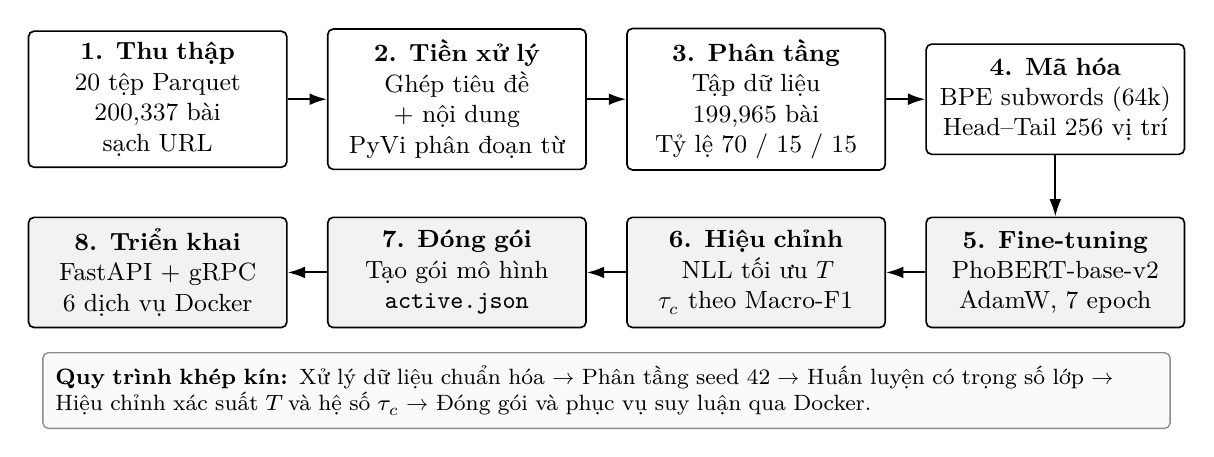
\begin{tikzpicture}
  % Row 1: Data Preparation & Preprocessing (Left to Right, y = 1.1)
  \node[arch_box, text width=30mm, minimum height=14mm] (p1) at (-5.7,1.1) {
    \textbf{1. Thu thập}\\
    20 tệp Parquet\\
    200,337 bài sạch URL
  };
  \node[arch_box, text width=30mm, minimum height=14mm] (p2) at (-1.9,1.1) {
    \textbf{2. Tiền xử lý}\\
    Ghép tiêu đề + nội dung\\
    PyVi phân đoạn từ
  };
  \node[arch_box, text width=30mm, minimum height=14mm] (p3) at (1.9,1.1) {
    \textbf{3. Phân tầng}\\
    Tập dữ liệu 199,965 bài\\
    Tỷ lệ 70 / 15 / 15
  };
  \node[arch_box, text width=30mm, minimum height=14mm] (p4) at (5.7,1.1) {
    \textbf{4. Mã hóa}\\
    BPE subwords (64k)\\
    Head--Tail 256 vị trí
  };

  % Row 2: Modeling, Calibration & Serving (Right to Left, y = -1.1)
  \node[arch_box_gray, text width=30mm, minimum height=14mm] (p5) at (5.7,-1.1) {
    \textbf{5. Fine-tuning}\\
    PhoBERT-base-v2\\
    AdamW, 7 epoch
  };
  \node[arch_box_gray, text width=30mm, minimum height=14mm] (p6) at (1.9,-1.1) {
    \textbf{6. Hiệu chỉnh}\\
    NLL tối ưu $T$\\
    $\tau_c$ theo Macro-F1
  };
  \node[arch_box_gray, text width=30mm, minimum height=14mm] (p7) at (-1.9,-1.1) {
    \textbf{7. Đóng gói}\\
    Tạo gói mô hình\\
    \texttt{active.json}
  };
  \node[arch_box_gray, text width=30mm, minimum height=14mm] (p8) at (-5.7,-1.1) {
    \textbf{8. Triển khai}\\
    FastAPI + gRPC\\
    6 dịch vụ Docker
  };

  % Strictly Orthogonal Connections (All horizontal gaps = 8mm, vertical drop = 8mm)
  \draw[arch_flow] (p1) -- (p2);
  \draw[arch_flow] (p2) -- (p3);
  \draw[arch_flow] (p3) -- (p4);
  \draw[arch_flow] (p4.south) -- (p5.north);
  \draw[arch_flow] (p5) -- (p6);
  \draw[arch_flow] (p6) -- (p7);
  \draw[arch_flow] (p7) -- (p8);

  % Bottom Invariant Badge
  \node[arch_badge, text width=140mm] (badge) at (0,-2.6) {
    \textbf{Quy trình khép kín:} Xử lý dữ liệu chuẩn hóa $\to$ Phân tầng seed 42 $\to$ Huấn luyện có trọng số lớp $\to$ Hiệu chỉnh xác suất $T$ và hệ số $\tau_c$ $\to$ Đóng gói và phục vụ suy luận qua Docker.
  };
\end{tikzpicture}
\caption{Quy trình NLP tổng thể từ dữ liệu thô đến hệ thống ứng dụng hỗ trợ biên tập.}
\end{figure}
}

% -----------------------------------------------------------------------------
% 2. SplitDiagram: Strict 3-Way Data Partitioning
% Node Sizes: Exactly 2 sizes:
%   - Size 1: Wide Banner (130mm x 11mm) for Master Corpus.
%   - Size 2: Partition & Role Boxes (38mm x 18mm) for all 6 columns.
% Fixed Spacing: dx = 48mm (gap = 10mm), dy = 26mm (gap = 8mm).
% -----------------------------------------------------------------------------
\newcommand{\SplitDiagram}{
\begin{figure}[tbp]\centering
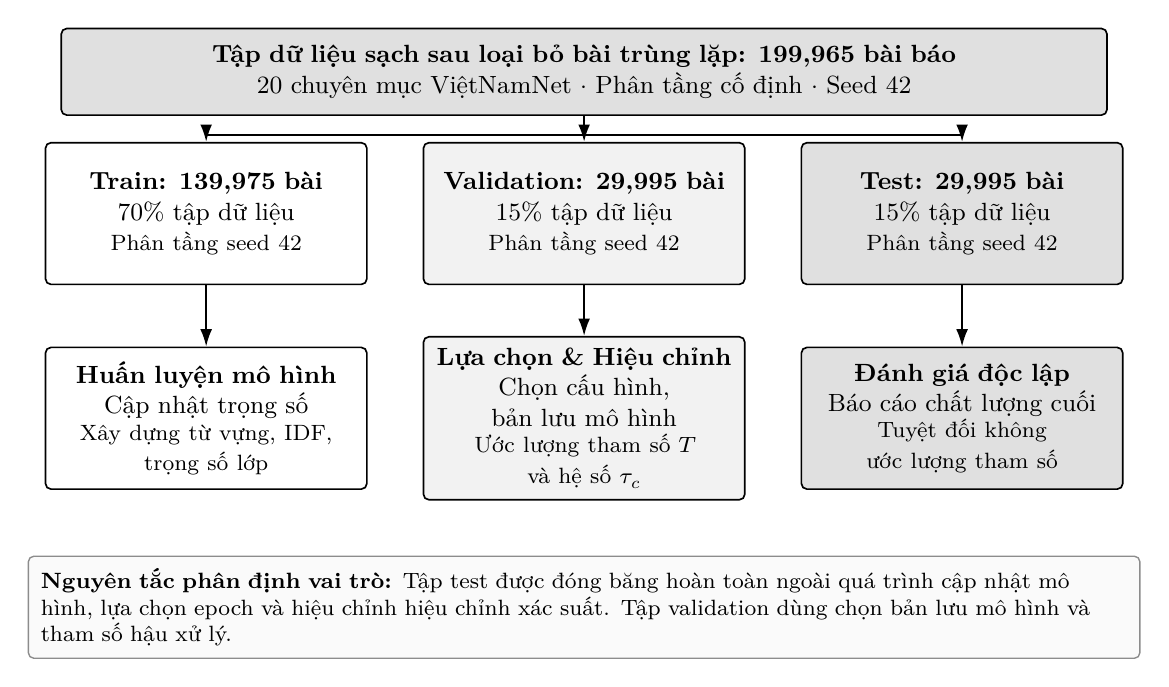
\begin{tikzpicture}
  % Stage 1: Filtered Master Corpus (y = 2.8)
  \node[arch_box_dark, text width=130mm, minimum height=11mm] (all) at (0,2.8) {
    \textbf{Tập dữ liệu sạch sau loại bỏ bài trùng lặp: 199,965 bài báo}\\
    20 chuyên mục ViệtNamNet $\cdot$ Phân tầng cố định $\cdot$ Seed 42
  };

  % Strictly Orthogonal Bus Coordinate (y = 2.0)
  \coordinate (splitbus) at (0,2.0);

  % Stage 2: Three Partitions (Symmetric, y = 1.0, height = 18mm)
  \node[arch_box, text width=38mm, minimum height=18mm] (train) at (-4.8,1.0) {
    \textbf{Train: 139,975 bài}\\
    \small 70\% tập dữ liệu\\
    \footnotesize Phân tầng seed 42
  };
  \node[arch_box_gray, text width=38mm, minimum height=18mm] (val) at (0,1.0) {
    \textbf{Validation: 29,995 bài}\\
    \small 15\% tập dữ liệu\\
    \footnotesize Phân tầng seed 42
  };
  \node[arch_box_dark, text width=38mm, minimum height=18mm] (test) at (4.8,1.0) {
    \textbf{Test: 29,995 bài}\\
    \small 15\% tập dữ liệu\\
    \footnotesize Phân tầng seed 42
  };

  % Stage 3: Operational Roles (y = -1.6, height = 18mm, exact 8mm gap from Row 2!)
  \node[arch_box, text width=38mm, minimum height=18mm] (fit) at (-4.8,-1.6) {
    \textbf{Huấn luyện mô hình}\\
    \small Cập nhật trọng số\\
    \footnotesize Xây dựng từ vựng, IDF,\\trọng số lớp
  };
  \node[arch_box_gray, text width=38mm, minimum height=18mm] (select) at (0,-1.6) {
    \textbf{Lựa chọn \& Hiệu chỉnh}\\
    \small Chọn cấu hình, bản lưu mô hình\\
    \footnotesize Ước lượng tham số $T$\\và hệ số $\tau_c$
  };
  \node[arch_box_dark, text width=38mm, minimum height=18mm] (score) at (4.8,-1.6) {
    \textbf{Đánh giá độc lập}\\
    \small Báo cáo chất lượng cuối\\
    \footnotesize Tuyệt đối không\\ước lượng tham số
  };

  % Strictly Orthogonal Bus Connections (Start on splitbus y=2.0)
  \draw[arch_line] (all.south) -- (splitbus);
  \draw[arch_line] (-4.8,2.0) -- (4.8,2.0);
  \draw[arch_flow] (-4.8,2.0) -- (train.north);
  \draw[arch_flow] (splitbus) -- (val.north);
  \draw[arch_flow] (4.8,2.0) -- (test.north);

  % Vertical Connections to Roles (Exact 8mm straight arrows)
  \draw[arch_flow] (train) -- (fit);
  \draw[arch_flow] (val) -- (select);
  \draw[arch_flow] (test) -- (score);

  % Bottom Invariant Badge (y = -4.0, generous 8mm clearance from role boxes)
  \node[arch_badge, text width=138mm] (badge) at (0,-4.0) {
    \textbf{Nguyên tắc phân định vai trò:} Tập test được đóng băng hoàn toàn ngoài quá trình cập nhật mô hình, lựa chọn epoch và hiệu chỉnh hiệu chỉnh xác suất. Tập validation dùng chọn bản lưu mô hình và tham số hậu xử lý.
  };
\end{tikzpicture}
\caption{Ba tập dữ liệu có vai trò tách biệt; tập test nằm ngoài cập nhật, chọn bản lưu mô hình và hiệu chỉnh.}
\end{figure}
}

% -----------------------------------------------------------------------------
% 3. PreprocessDiagram: Text Normalization Pipeline
% Node Sizes: Exactly 1 size (128mm x 11mm) for all 4 stages.
% Fixed Spacing: node distance = 7mm.
% -----------------------------------------------------------------------------
\newcommand{\PreprocessDiagram}{
\begin{figure}[tbp]\centering
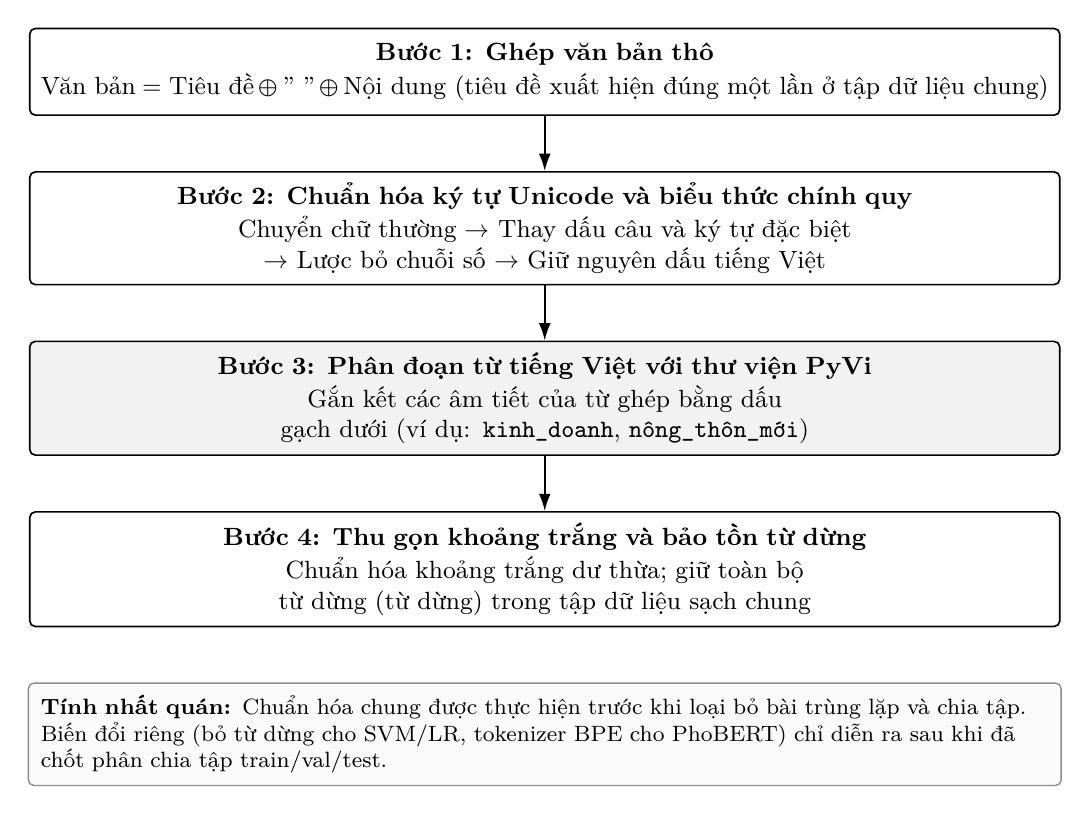
\begin{tikzpicture}[node distance=7mm]
  % Stage 1: Input text assembly
  \node[arch_box, text width=128mm, minimum height=11mm] (s1) {
    \textbf{Bước 1: Ghép văn bản thô}\\[1pt]
    $\text{Văn bản} = \text{Tiêu đề} \oplus \text{" "} \oplus \text{Nội dung}$ (tiêu đề xuất hiện đúng một lần ở tập dữ liệu chung)
  };

  % Stage 2: Normalization
  \node[arch_box, text width=128mm, minimum height=11mm, below=of s1] (s2) {
    \textbf{Bước 2: Chuẩn hóa ký tự Unicode và biểu thức chính quy}\\[1pt]
    Chuyển chữ thường $\to$ Thay dấu câu và ký tự đặc biệt $\to$ Lược bỏ chuỗi số $\to$ Giữ nguyên dấu tiếng Việt
  };

  % Stage 3: Word Segmentation
  \node[arch_box_gray, text width=128mm, minimum height=11mm, below=of s2] (s3) {
    \textbf{Bước 3: Phân đoạn từ tiếng Việt với thư viện PyVi}\\[1pt]
    Gắn kết các âm tiết của từ ghép bằng dấu gạch dưới (ví dụ: \texttt{kinh\_doanh}, \texttt{nông\_thôn\_mới})
  };

  % Stage 4: Whitespace and Corpus Delivery
  \node[arch_box, text width=128mm, minimum height=11mm, below=of s3] (s4) {
    \textbf{Bước 4: Thu gọn khoảng trắng và bảo tồn từ dừng}\\[1pt]
    Chuẩn hóa khoảng trắng dư thừa; giữ toàn bộ từ dừng (từ dừng) trong tập dữ liệu sạch chung
  };

  % Strictly Orthogonal Straight Arrows (Fixed 7mm length)
  \draw[arch_flow] (s1) -- (s2);
  \draw[arch_flow] (s2) -- (s3);
  \draw[arch_flow] (s3) -- (s4);

  % Bottom Badge
  \node[arch_badge, text width=128mm, below=7mm of s4] (b) {
    \textbf{Tính nhất quán:} Chuẩn hóa chung được thực hiện trước khi loại bỏ bài trùng lặp và chia tập. Biến đổi riêng (bỏ từ dừng cho SVM/LR, tokenizer BPE cho PhoBERT) chỉ diễn ra sau khi đã chốt phân chia tập train/val/test.
  };
\end{tikzpicture}
\caption{Chuẩn hóa chung trước loại bỏ bài trùng lặp; biến đổi riêng của từng mô hình diễn ra sau khi chốt tập dữ liệu.}\label{fig:preprocess}
\end{figure}
}

% -----------------------------------------------------------------------------
% 4. CorpusAuditDiagram: Data Cleaning Tree
% Node Sizes: Exactly 2 sizes:
%   - Size 1: Wide Banner (128mm x 12mm) for Stages 1, 2, 4, 5, 6.
%   - Size 2: Column Box (38mm x 15mm) for Stage 3 (3 branches).
% Fixed Spacing: Symmetric center at x = 0, fixed vertical steps.
% -----------------------------------------------------------------------------
\newcommand{\CorpusAuditDiagram}{
\begin{figure}[tbp]\centering
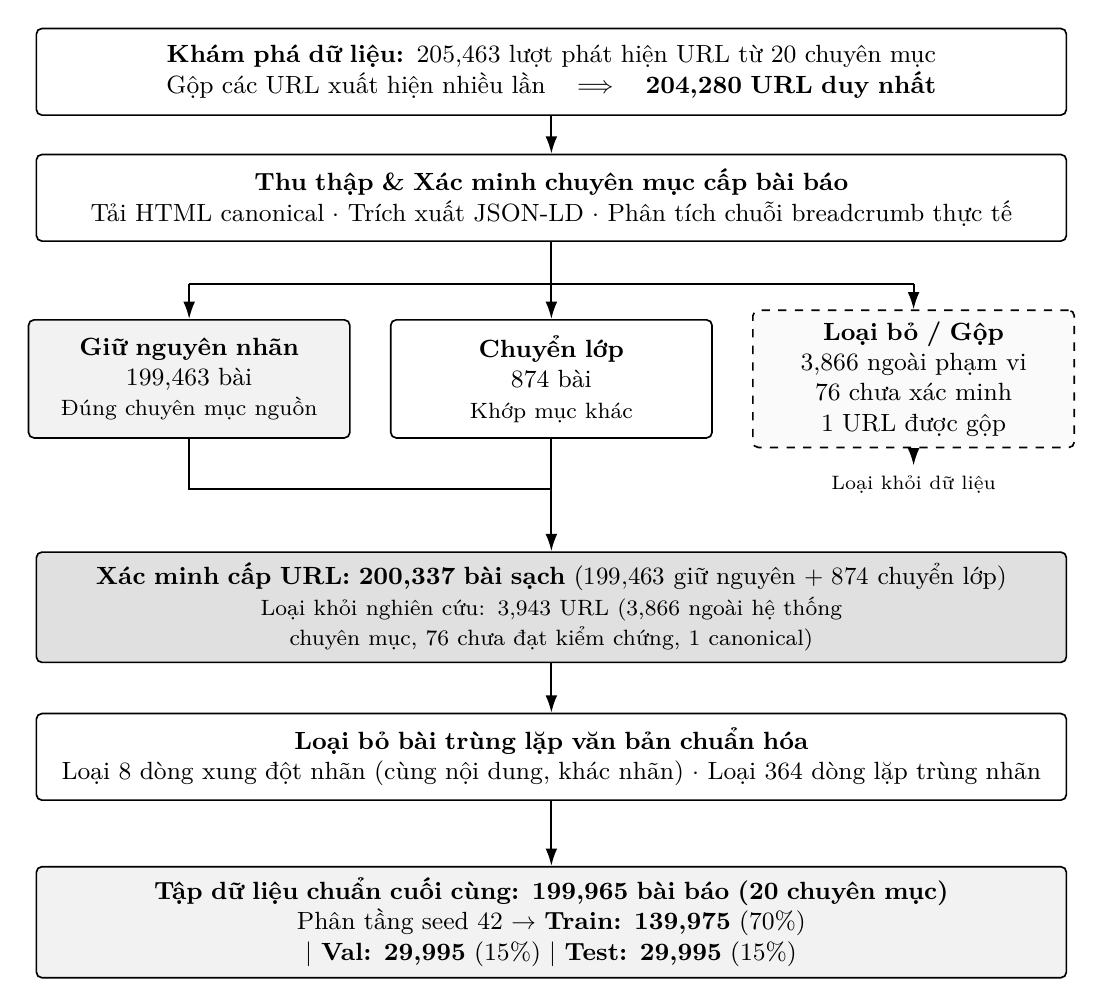
\begin{tikzpicture}
  % Stage 1: Raw Discovery (y = 5.5)
  \node[arch_box, text width=128mm, minimum height=11mm] (raw) at (0,5.5) {
    \textbf{Khám phá dữ liệu:} 205,463 lượt phát hiện URL từ 20 chuyên mục\\
    Gộp các URL xuất hiện nhiều lần $\implies$ \textbf{204,280 URL duy nhất}
  };

  % Stage 2: HTML Extraction & Verification (y = 3.9, 5mm gap from raw)
  \node[arch_box, text width=128mm, minimum height=11mm] (verify) at (0,3.9) {
    \textbf{Thu thập \& Xác minh chuyên mục cấp bài báo}\\
    Tải HTML canonical $\cdot$ Trích xuất \mbox{JSON-LD} $\cdot$ Phân tích chuỗi breadcrumb thực tế
  };

  % Stage 3: Three Branches (y = 1.6, height = 15mm)
  \node[arch_box_gray, text width=38mm, minimum height=15mm] (same) at (-4.6,1.6) {
    \textbf{Giữ nguyên nhãn}\\
    199,463 bài\\
    \footnotesize Đúng chuyên mục nguồn
  };
  \node[arch_box, text width=38mm, minimum height=15mm] (move) at (0,1.6) {
    \textbf{Chuyển lớp}\\
    874 bài\\
    \footnotesize Khớp mục khác
  };
  \node[arch_box_dashed, text width=38mm, minimum height=15mm] (drop) at (4.6,1.6) {
    \textbf{Loại bỏ / Gộp}\\
    3,866 ngoài phạm vi\\
    76 chưa xác minh\\
    1 URL được gộp
  };

  % Stage 4: Clean URL Aggregation (Wide Banner, y = -1.3, height = 12mm)
  \node[arch_box_dark, text width=128mm, minimum height=12mm] (clean) at (0,-1.3) {
    \textbf{Xác minh cấp URL: 200,337 bài sạch} ($199{,}463\text{ giữ nguyên} + 874\text{ chuyển lớp}$)\\
    \footnotesize Loại khỏi nghiên cứu: 3,943 URL (3,866 ngoài hệ thống chuyên mục, 76 chưa đạt kiểm chứng, 1 canonical)
  };

  % Stage 5: Text Deduplication (Wide Banner, y = -3.2, height = 11mm)
  \node[arch_box, text width=128mm, minimum height=11mm] (dedup) at (0,-3.2) {
    \textbf{Loại bỏ bài trùng lặp văn bản chuẩn hóa}\\
    Loại 8 dòng xung đột nhãn (cùng nội dung, khác nhãn) $\cdot$ Loại 364 dòng lặp trùng nhãn
  };

  % Stage 6: Final Corpus & Split (Wide Banner, y = -5.3, height = 12mm)
  \node[arch_box_gray, text width=128mm, minimum height=12mm] (corpus) at (0,-5.3) {
    \textbf{Tập dữ liệu chuẩn cuối cùng: 199,965 bài báo (20 chuyên mục)}\\
    Phân tầng seed 42 $\to$ \textbf{Train: 139,975} (70\%) $\mid$ \textbf{Val: 29,995} (15\%) $\mid$ \textbf{Test: 29,995} (15\%)
  };

  % Routing: Strictly Orthogonal
  \draw[arch_flow] (raw) -- (verify);

  % Branching from verify (bus at y = 2.8)
  \coordinate (vbus) at (0, 2.8);
  \draw[arch_line] (verify.south) -- (vbus);
  \draw[arch_line] (-4.6, 2.8) -- (4.6, 2.8);
  \draw[arch_flow] (-4.6, 2.8) -- (same.north);
  \draw[arch_flow] (vbus) -- (move.north);
  \draw[arch_flow] (4.6, 2.8) -- (drop.north);

  % Merging branches: 'same' and 'move' merge into clean (bus at y = 0.2)
  \coordinate (cbus) at (0, 0.2);
  \draw[arch_line] (same.south) -- (-4.6, 0.2) -- (cbus);
  \draw[arch_line] (move.south) -- (cbus);
  \draw[arch_flow] (cbus) -- (clean.north);

  % Excluded branch: drop terminates outside with generous clearance from clean
  \draw[arch_flow, dashed] (drop.south) -- (4.6, 0.5) node[below, font=\scriptsize] {Loại khỏi dữ liệu};

  % Sequential Spine: Clean to Dedup to Corpus (Strictly vertical straight drops)
  \draw[arch_flow] (clean) -- (dedup);
  \draw[arch_flow] (dedup) -- (corpus);

\end{tikzpicture}
\caption{Xác minh chuyên mục và tạo tập dữ liệu; nhánh loại/gộp không đi vào dữ liệu huấn luyện.}\label{fig:corpus-audit}
\end{figure}
}

% -----------------------------------------------------------------------------
% 5. MethodFamiliesDiagram: 3 Representation Families & 4 Models
% Node Sizes: Exactly 2 sizes:
%   - Size 1: Wide Banner (136mm x 10mm) for Input and Output.
%   - Size 2: Grid Column Box (42mm x 16mm) for all 9 intermediate nodes.
% Fixed Spacing: dx = 47mm (gap = 5mm), dy = 22mm (gap = 6mm).
% -----------------------------------------------------------------------------
\newcommand{\MethodFamiliesDiagram}{
\begin{figure}[tbp]\centering
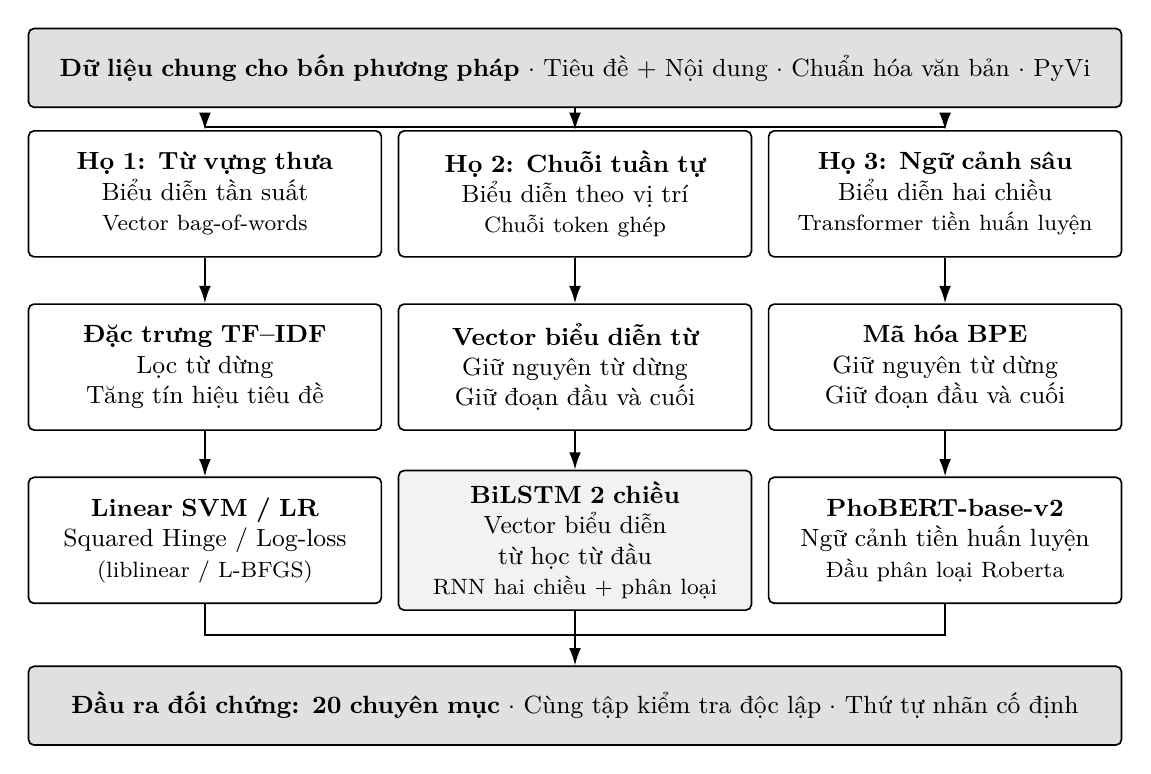
\begin{tikzpicture}
  % Common Input Node (y = 0)
  \node[arch_box_dark, text width=136mm, minimum height=10mm] (input) at (0,0) {
    \textbf{Dữ liệu chung cho bốn phương pháp} $\cdot$ Tiêu đề + Nội dung $\cdot$ Chuẩn hóa văn bản $\cdot$ PyVi
  };

  % Level 1: Representation Families (y = -1.6, height = 16mm)
  \node[arch_box, text width=42mm, minimum height=16mm] (fam1) at (-4.7,-1.6) {
    \textbf{Họ 1: Từ vựng thưa}\\
    \small Biểu diễn tần suất\\
    \footnotesize Vector bag-of-words
  };
  \node[arch_box, text width=42mm, minimum height=16mm] (fam2) at (0,-1.6) {
    \textbf{Họ 2: Chuỗi tuần tự}\\
    \small Biểu diễn theo vị trí\\
    \footnotesize Chuỗi token ghép
  };
  \node[arch_box, text width=42mm, minimum height=16mm] (fam3) at (4.7,-1.6) {
    \textbf{Họ 3: Ngữ cảnh sâu}\\
    \small Biểu diễn hai chiều\\
    \footnotesize Transformer tiền huấn luyện
  };

  % Level 2: Features & Vocabularies (y = -3.8, height = 16mm, exact 6mm gap!)
  \node[arch_box, text width=42mm, minimum height=16mm] (rep1) at (-4.7,-3.8) {
    \textbf{Đặc trưng TF--IDF}\\
    Lọc từ dừng\\
    Tăng tín hiệu tiêu đề
  };
  \node[arch_box, text width=42mm, minimum height=16mm] (rep2) at (0,-3.8) {
    \textbf{Vector biểu diễn từ}\\
    Giữ nguyên từ dừng\\
    Giữ đoạn đầu và cuối
  };
  \node[arch_box, text width=42mm, minimum height=16mm] (rep3) at (4.7,-3.8) {
    \textbf{Mã hóa BPE}\\
    Giữ nguyên từ dừng\\
    Giữ đoạn đầu và cuối
  };

  % Level 3: Model Architectures (y = -6.0, height = 16mm, exact 6mm gap!)
  \node[arch_box, text width=42mm, minimum height=16mm] (mod1) at (-4.7,-6.0) {
    \textbf{Linear SVM / LR}\\
    \small Squared Hinge / Log-loss\\
    \footnotesize (liblinear / L-BFGS)
  };
  \node[arch_box_gray, text width=42mm, minimum height=16mm] (mod2) at (0,-6.0) {
    \textbf{BiLSTM 2 chiều}\\
    \small Vector biểu diễn từ học từ đầu\\
    \footnotesize RNN hai chiều + phân loại
  };
  \node[arch_box, text width=42mm, minimum height=16mm] (mod3) at (4.7,-6.0) {
    \textbf{PhoBERT-base-v2}\\
    \small Ngữ cảnh tiền huấn luyện\\
    \footnotesize Đầu phân loại Roberta
  };

  % Common Output Node (y = -8.1, height = 10mm)
  \node[arch_box_dark, text width=136mm, minimum height=10mm] (out) at (0,-8.1) {
    \textbf{Đầu ra đối chứng: 20 chuyên mục} $\cdot$ Cùng tập kiểm tra độc lập $\cdot$ Thứ tự nhãn cố định
  };

  % Top Bus at y = -0.75
  \coordinate (inbus) at (0,-0.75);
  \draw[arch_line] (input.south) -- (inbus);
  \draw[arch_line] (-4.7,-0.75) -- (4.7,-0.75);
  \draw[arch_flow] (-4.7,-0.75) -- (fam1.north);
  \draw[arch_flow] (inbus) -- (fam2.north);
  \draw[arch_flow] (4.7,-0.75) -- (fam3.north);

  % Vertical Sequential Flows (All exact 6mm vertical arrows)
  \draw[arch_flow] (fam1) -- (rep1);
  \draw[arch_flow] (rep1) -- (mod1);

  \draw[arch_flow] (fam2) -- (rep2);
  \draw[arch_flow] (rep2) -- (mod2);

  \draw[arch_flow] (fam3) -- (rep3);
  \draw[arch_flow] (rep3) -- (mod3);

  % Bottom Bus at y = -7.2 (Strictly Orthogonal)
  \coordinate (outbus) at (0,-7.2);
  \draw[arch_line] (mod1.south) |- (outbus);
  \draw[arch_line] (mod2.south) -- (outbus);
  \draw[arch_line] (mod3.south) |- (outbus);
  \draw[arch_flow] (outbus) -- (out.north);

\end{tikzpicture}
\caption{Ba họ biểu diễn và bốn quy trình phân loại. Phần văn bản quan sát, tiền huấn luyện và ngân sách tối ưu khác nhau.}\label{fig:method_families}
\end{figure}
}

% -----------------------------------------------------------------------------
% 6. BiLSTMDiagram: BiLSTM Baseline Architecture (Figure fig:bilstm_arch)
% Node Sizes: Exactly 1 rectangular size (21mm x 14mm) for all 6 stages.
% Fixed Spacing: Clean 6mm horizontal gaps between all nodes.
% -----------------------------------------------------------------------------
\newcommand{\BiLSTMDiagram}{
\begin{figure}[tbp]\centering
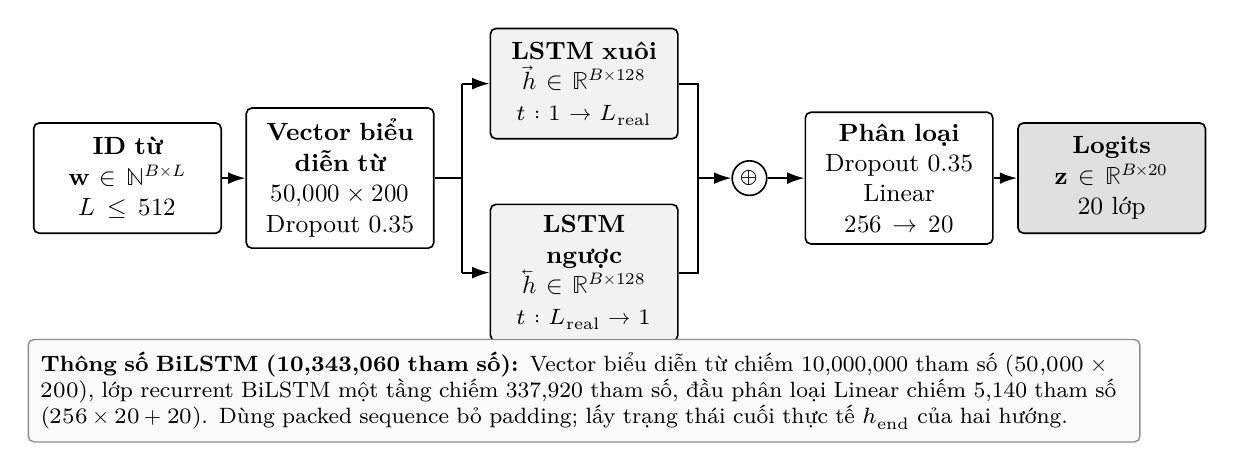
\begin{tikzpicture}
  % Input Tokens (center -5.8, width 21mm -> [-6.85, -4.75])
  \node[arch_box, text width=21mm, minimum height=14mm] (tok) at (-5.8,0) {
    \textbf{ID từ}\\
    $\mathbf{w} \in \mathbb{N}^{B \times L}$\\
    $L \le 512$
  };

  % Word Embedding (center -3.1, width 21mm -> [-4.15, -2.05])
  \node[arch_box, text width=21mm, minimum height=14mm] (emb) at (-3.1,0) {
    \textbf{Vector biểu diễn từ}\\
    $50{,}000 \times 200$\\
    Dropout 0.35
  };

  % BiLSTM Recurrent Layers (center 0.0, width 21mm -> [-1.05, +1.05])
  \node[arch_box_gray, text width=21mm, minimum height=14mm] (fw) at (0,1.2) {
    \textbf{LSTM xuôi}\\
    $\overrightarrow{h} \in \mathbb{R}^{B \times 128}$\\
    \footnotesize $t: 1 \to L_{\text{real}}$
  };
  \node[arch_box_gray, text width=21mm, minimum height=14mm] (bw) at (0,-1.2) {
    \textbf{LSTM ngược}\\
    $\overleftarrow{h} \in \mathbb{R}^{B \times 128}$\\
    \footnotesize $t: L_{\text{real}} \to 1$
  };

  % Concatenation Operator (diameter 6mm, center at x = 2.1)
  \node[arch_op] (cat) at (2.1,0) {$\oplus$};

  % Classification Head (center 4.0, width 21mm -> [2.95, 5.05])
  \node[arch_box, text width=21mm, minimum height=14mm] (head) at (4.0,0) {
    \textbf{Phân loại}\\
    Dropout 0.35\\
    Linear $256 \to 20$
  };

  % Logits Output (center 6.7, width 21mm -> [5.65, 7.75])
  \node[arch_box_dark, text width=21mm, minimum height=14mm] (out) at (6.7,0) {
    \textbf{Logits}\\
    $\mathbf{z} \in \mathbb{R}^{B \times 20}$\\
    20 lớp
  };

  % Strictly Orthogonal Routing: tok to emb (6mm clean arrow)
  \draw[arch_flow] (tok) -- (emb);

  % Emb to Forward and Backward: Split bus at x = -1.55 (5mm from emb.east, 5mm from fw.west!)
  \coordinate (emb_split) at (-1.55, 0);
  \draw[arch_line] (emb.east) -- (emb_split);
  \draw[arch_line] (emb_split) -- (-1.55, 1.2);
  \draw[arch_flow] (-1.55, 1.2) -- (fw.west);
  \draw[arch_line] (emb_split) -- (-1.55, -1.2);
  \draw[arch_flow] (-1.55, -1.2) -- (bw.west);

  % Forward and Backward to Concat: Join bus at x = 1.45 (4mm from fw.east, 4mm from cat.west!)
  \coordinate (cat_join) at (1.45, 0);
  \draw[arch_line] (fw.east) -- (1.45, 1.2) -- (cat_join);
  \draw[arch_line] (bw.east) -- (1.45, -1.2) -- (cat_join);
  \draw[arch_flow] (cat_join) -- (cat.west);

  % Concat to Head (6mm clean arrow)
  \draw[arch_flow] (cat) -- (head);

  % Head to Out (6mm clean arrow)
  \draw[arch_flow] (head) -- (out);

  % Bottom Parameter Badge (y = -2.7, generous clearance)
  \node[arch_badge, text width=138mm] (badge) at (0,-2.7) {
    \textbf{Thông số BiLSTM (10,343,060 tham số):} Vector biểu diễn từ chiếm 10,000,000 tham số ($50{,}000 \times 200$), lớp recurrent BiLSTM một tầng chiếm 337,920 tham số, đầu phân loại Linear chiếm 5,140 tham số ($256 \times 20 + 20$). Dùng packed sequence bỏ padding; lấy trạng thái cuối thực tế $h_{\text{end}}$ của hai hướng.
  };
\end{tikzpicture}
\caption{BiLSTM thực thi trong notebook: vector biểu diễn từ học từ đầu, packed sequence, ghép hidden cuối hai hướng và đầu phân loại 20 lớp. Dropout vector biểu diễn từ được lược trong khối để giữ sơ đồ gọn.}\label{fig:bilstm_arch}
\end{figure}
}

% -----------------------------------------------------------------------------
% 7. HeadTailDiagram: PhoBERT Head-Tail Truncation
% Node Sizes: Exactly 2 sizes:
%   - Size 1: Wide Banner (138mm x 9mm) for Raw BPE Sequence.
%   - Size 2: Uniform Segment Box (22mm x 14mm) for each segment.
% -----------------------------------------------------------------------------
\newcommand{\HeadTailDiagram}{
\begin{figure}[tbp]\centering
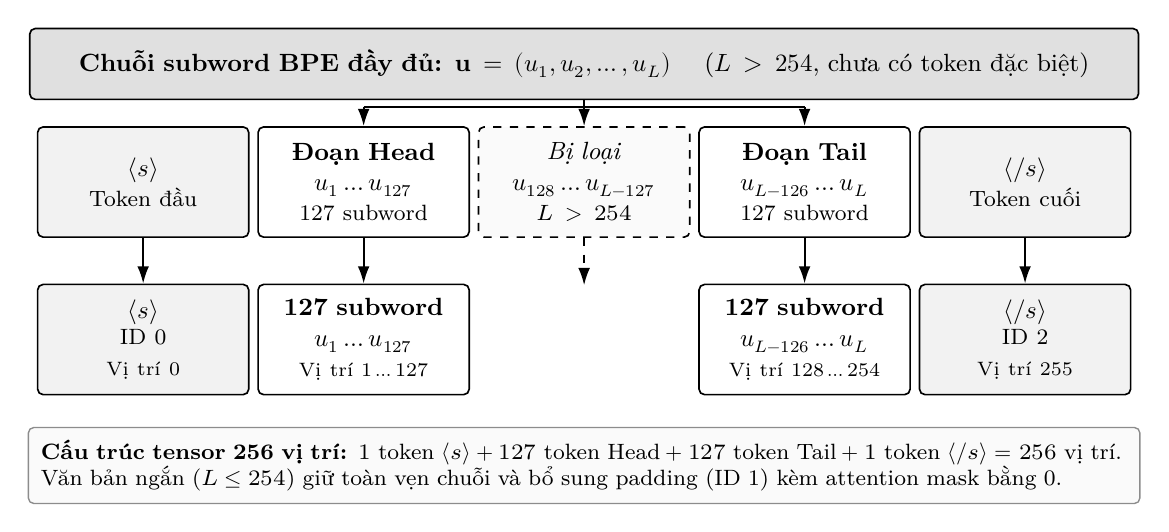
\begin{tikzpicture}
  % Top: Raw BPE Sequence Representation (Wide Banner, y = 2.5)
  \node[arch_box_dark, text width=138mm, minimum height=9mm] (raw) at (0,2.5) {
    \textbf{Chuỗi subword BPE đầy đủ:} $\mathbf{u} = (u_1, u_2, \ldots, u_L)$ \quad ($L > 254$, chưa có token đặc biệt)
  };

  % Visual Partitioning (y = 1.0, 5 identical 24mm boxes, uniform 4mm gap)
  \node[arch_box_gray, text width=24mm, minimum height=14mm] (p_cls) at (-5.6,1.0) {
    $\langle s\rangle$\\
    \footnotesize Token đầu
  };
  \node[arch_box, text width=24mm, minimum height=14mm] (p_head) at (-2.8,1.0) {
    \textbf{Đoạn Head}\\
    $u_1 \dots u_{127}$\\
    \footnotesize 127 subword
  };
  \node[arch_box_dashed, text width=24mm, minimum height=14mm] (p_mid) at (0,1.0) {
    \textit{Bị loại}\\
    \small $u_{128} \dots u_{L-127}$\\
    \footnotesize $L > 254$
  };
  \node[arch_box, text width=24mm, minimum height=14mm] (p_tail) at (2.8,1.0) {
    \textbf{Đoạn Tail}\\
    $u_{L-126} \dots u_L$\\
    \footnotesize 127 subword
  };
  \node[arch_box_gray, text width=24mm, minimum height=14mm] (p_sep) at (5.6,1.0) {
    $\langle/ s\rangle$\\
    \footnotesize Token cuối
  };

  % Bottom: Assembled 256-token Tensor (y = -1.0, 8mm gap from Row 1!)
  \node[arch_box_gray, text width=24mm, minimum height=14mm] (t_cls) at (-5.6,-1.0) {
    $\langle s\rangle$\\
    \footnotesize ID 0\\
    \scriptsize Vị trí 0
  };
  \node[arch_box, text width=24mm, minimum height=14mm] (t_head) at (-2.8,-1.0) {
    \textbf{127 subword}\\
    $u_1 \dots u_{127}$\\
    \scriptsize Vị trí $1 \dots 127$
  };
  \node[arch_box, text width=24mm, minimum height=14mm] (t_tail) at (2.8,-1.0) {
    \textbf{127 subword}\\
    $u_{L-126} \dots u_L$\\
    \scriptsize Vị trí $128 \dots 254$
  };
  \node[arch_box_gray, text width=24mm, minimum height=14mm] (t_sep) at (5.6,-1.0) {
    $\langle/ s\rangle$\\
    \footnotesize ID 2\\
    \scriptsize Vị trí 255
  };

  % Orthogonal Routing: Top to Partition
  \coordinate (rawbus) at (0, 1.95);
  \draw[arch_line] (raw.south) -- (rawbus);
  \draw[arch_line] (-2.8, 1.95) -- (2.8, 1.95);
  \draw[arch_flow] (-2.8, 1.95) -- (p_head.north);
  \draw[arch_flow] (2.8, 1.95) -- (p_tail.north);
  \draw[arch_flow] (rawbus) -- (p_mid.north);

  % Strictly Vertical Straight Drops to Assembled Tensor (8mm vertical arrows)
  \draw[arch_flow] (p_cls) -- (t_cls);
  \draw[arch_flow] (p_head) -- (t_head);
  \draw[arch_flow] (p_tail) -- (t_tail);
  \draw[arch_flow] (p_sep) -- (t_sep);

  % Middle omission drop (dashed)
  \draw[arch_flow, dashed] (p_mid.south) -- ++(0,-0.6);

  % Invariant Badge (y = -2.6)
  \node[arch_badge, text width=138mm] (b) at (0,-2.6) {
    \textbf{Cấu trúc tensor 256 vị trí:} $1 \text{ token } \langle s\rangle + 127 \text{ token Head} + 127 \text{ token Tail} + 1 \text{ token } \langle/ s\rangle = 256 \text{ vị trí}$. Văn bản ngắn ($L \le 254$) giữ toàn vẹn chuỗi và bổ sung padding (ID 1) kèm attention mask bằng 0.
  };
\end{tikzpicture}
\caption{Cách ghép Head--Tail; dấu token được minh họa theo ký hiệu của tokenizer PhoBERT.}
\end{figure}
}

% -----------------------------------------------------------------------------
% 8. EncoderDiagram: PhoBERT Architecture & Classification Head
% Node Sizes: Exactly 1 size (128mm x 11mm) for all 6 stages.
% Fixed Spacing: node distance = 6mm.
% -----------------------------------------------------------------------------
\newcommand{\EncoderDiagram}{
\begin{figure}[tbp]\centering
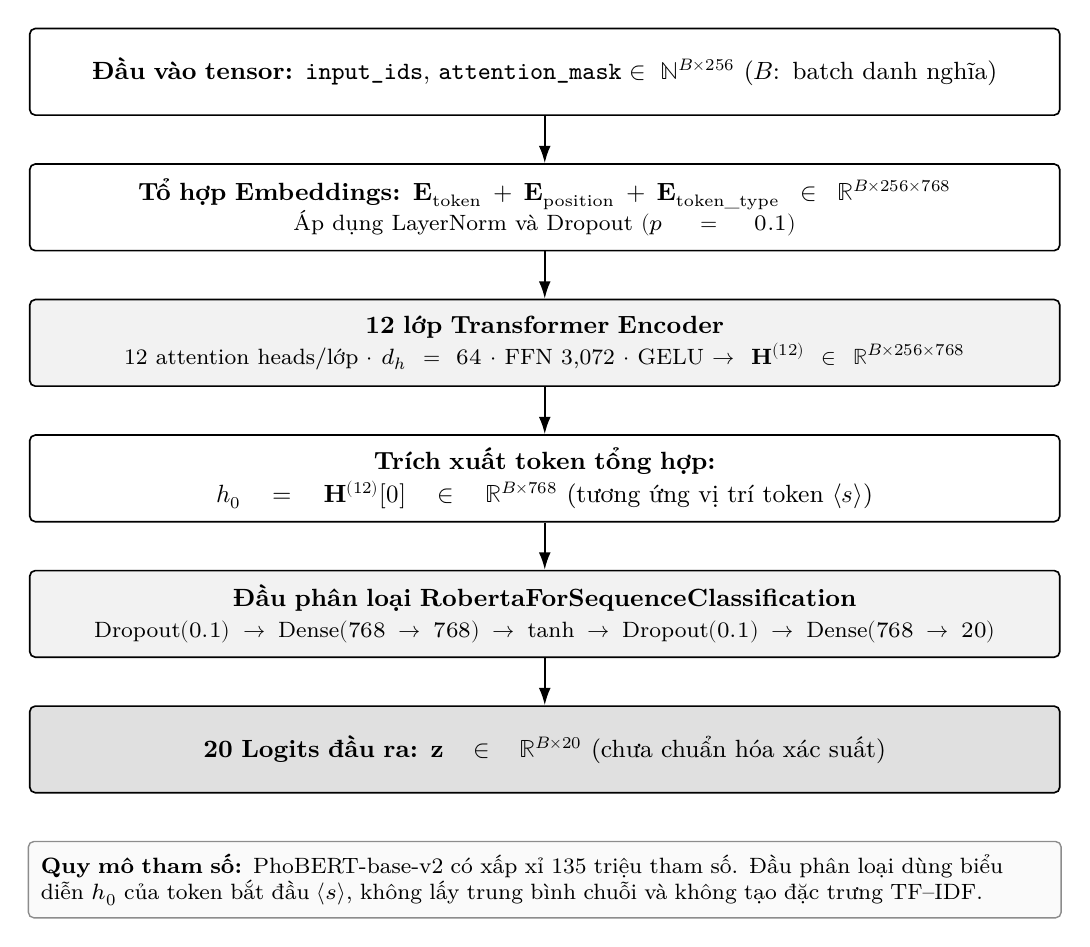
\begin{tikzpicture}[node distance=6mm]
  % Stage 1: Input Tensors
  \node[arch_box, text width=128mm, minimum height=11mm] (e1) {
    \textbf{Đầu vào tensor:} \texttt{input\_ids}, \texttt{attention\_mask} $\in \mathbb{N}^{B \times 256}$ ($B$: batch danh nghĩa)
  };

  % Stage 2: Embeddings
  \node[arch_box, text width=128mm, minimum height=11mm, below=of e1] (e2) {
    \textbf{Tổ hợp Embeddings:} $\mathbf{E}_{\text{token}} + \mathbf{E}_{\text{position}} + \mathbf{E}_{\text{token\_type}} \in \mathbb{R}^{B \times 256 \times 768}$\\
    \footnotesize Áp dụng LayerNorm và Dropout $(p=0.1)$
  };

  % Stage 3: Transformer Stack
  \node[arch_box_gray, text width=128mm, minimum height=11mm, below=of e2] (e3) {
    \textbf{12 lớp Transformer Encoder}\\
    \footnotesize 12 attention heads/lớp $\cdot$ $d_h=64$ $\cdot$ FFN 3,072 $\cdot$ GELU $\to \mathbf{H}^{(12)} \in \mathbb{R}^{B \times 256 \times 768}$
  };

  % Stage 4: First Token Extraction
  \node[arch_box, text width=128mm, minimum height=11mm, below=of e3] (e4) {
    \textbf{Trích xuất token tổng hợp:}\\[1pt]
    $h_0 = \mathbf{H}^{(12)}[0] \in \mathbb{R}^{B \times 768}$ (tương ứng vị trí token $\langle s\rangle$)
  };

  % Stage 5: Classification Head
  \node[arch_box_gray, text width=128mm, minimum height=11mm, below=of e4] (e5) {
    \textbf{Đầu phân loại RobertaForSequenceClassification}\\
    \footnotesize $\text{Dropout}(0.1) \to \text{Dense}(768 \to 768) \to \tanh \to \text{Dropout}(0.1) \to \text{Dense}(768 \to 20)$
  };

  % Stage 6: Output Logits
  \node[arch_box_dark, text width=128mm, minimum height=11mm, below=of e5] (e6) {
    \textbf{20 Logits đầu ra:} $\mathbf{z} \in \mathbb{R}^{B \times 20}$ (chưa chuẩn hóa xác suất)
  };

  % Strictly Orthogonal Straight Connections (All fixed 6mm vertical arrows)
  \draw[arch_flow] (e1) -- (e2);
  \draw[arch_flow] (e2) -- (e3);
  \draw[arch_flow] (e3) -- (e4);
  \draw[arch_flow] (e4) -- (e5);
  \draw[arch_flow] (e5) -- (e6);

  % Badge
  \node[arch_badge, text width=128mm, below=6mm of e6] (b) {
    \textbf{Quy mô tham số:} PhoBERT-base-v2 có xấp xỉ 135 triệu tham số. Đầu phân loại dùng biểu diễn $h_0$ của token bắt đầu $\langle s\rangle$, không lấy trung bình chuỗi và không tạo đặc trưng TF--IDF.
  };
\end{tikzpicture}
\caption{PhoBERT và đầu phân loại trong RobertaForSequenceClassification.}
\end{figure}
}

% -----------------------------------------------------------------------------
% 9. AttentionDiagram: Scaled Dot-Product & Multi-Head Attention
% Node Sizes: Exactly 2 sizes:
%   - Size 1: Wide Layer Box (112mm x 12mm) for H, Att, Res1, Res2, Out.
%   - Size 2: Projection Box (24mm x 12mm) for Q, K, V.
% Fixed Spacing: Symmetric center at x = 0, fixed vertical spacing.
% -----------------------------------------------------------------------------
\newcommand{\AttentionDiagram}{
\begin{figure}[tbp]\centering
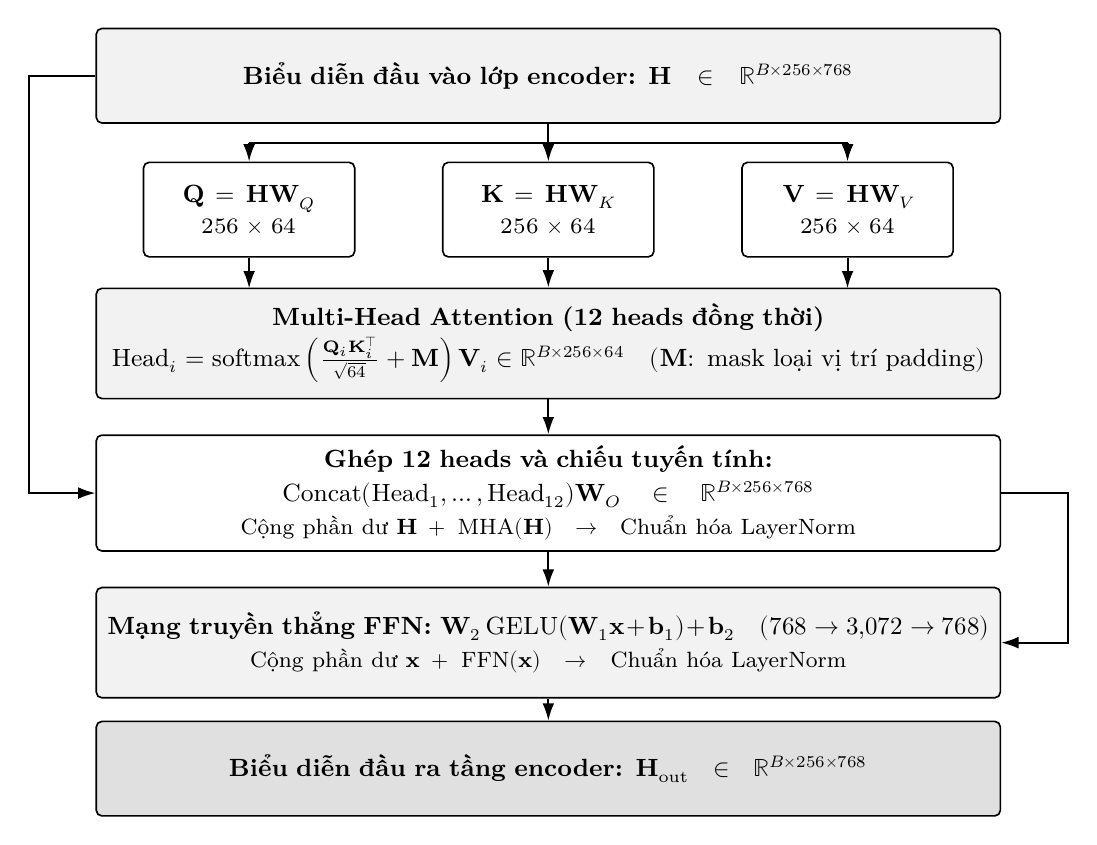
\begin{tikzpicture}
  % Stage 1: Input Hidden States (y = 4.4, width 112mm -> [-5.6, +5.6])
  \node[arch_box_gray, text width=112mm, minimum height=12mm] (h) at (0,4.4) {
    \textbf{Biểu diễn đầu vào lớp encoder:} $\mathbf{H} \in \mathbb{R}^{B \times 256 \times 768}$
  };

  % Stage 2: Linear Projections for Q, K, V (y = 2.7, width 24mm each)
  \node[arch_box, text width=24mm, minimum height=12mm] (q) at (-3.8,2.7) {
    $\mathbf{Q} = \mathbf{H}\mathbf{W}_Q$\\
    \footnotesize $256 \times 64$
  };
  \node[arch_box, text width=24mm, minimum height=12mm] (k) at (0,2.7) {
    $\mathbf{K} = \mathbf{H}\mathbf{W}_K$\\
    \footnotesize $256 \times 64$
  };
  \node[arch_box, text width=24mm, minimum height=12mm] (v) at (3.8,2.7) {
    $\mathbf{V} = \mathbf{H}\mathbf{W}_V$\\
    \footnotesize $256 \times 64$
  };

  % Stage 3: Multi-Head Scaled Dot-Product Attention (y = 1.0, width 112mm)
  \node[arch_box_gray, text width=112mm, minimum height=14mm] (att) at (0,1.0) {
    \textbf{Multi-Head Attention (12 heads đồng thời)}\\[1pt]
    $\text{Head}_i = \operatorname{softmax}\left(\frac{\mathbf{Q}_i \mathbf{K}_i^\top}{\sqrt{64}} + \mathbf{M}\right)\mathbf{V}_i \in \mathbb{R}^{B \times 256 \times 64} \quad (\mathbf{M}\text{: mask loại vị trí padding})$
  };

  % Stage 4: Projection, Residual Connection & LayerNorm (y = -0.9, width 112mm)
  \node[arch_box, text width=112mm, minimum height=14mm] (res1) at (0,-0.9) {
    \textbf{Ghép 12 heads và chiếu tuyến tính:}\\[1pt]
    $\operatorname{Concat}(\text{Head}_1, \ldots, \text{Head}_{12})\mathbf{W}_O \in \mathbb{R}^{B \times 256 \times 768}$\\[1pt]
    \footnotesize Cộng phần dư $\mathbf{H} + \text{MHA}(\mathbf{H}) \to \text{Chuẩn hóa LayerNorm}$
  };

  % Stage 5: Feed-Forward Network & LayerNorm (y = -2.8, width 112mm)
  \node[arch_box_gray, text width=112mm, minimum height=14mm] (res2) at (0,-2.8) {
    \textbf{Mạng truyền thẳng FFN:} $\mathbf{W}_2\operatorname{GELU}(\mathbf{W}_1 \mathbf{x} + \mathbf{b}_1) + \mathbf{b}_2 \quad (768 \to 3{,}072 \to 768)$\\[1pt]
    \footnotesize Cộng phần dư $\mathbf{x} + \text{FFN}(\mathbf{x}) \to \text{Chuẩn hóa LayerNorm}$
  };

  % Stage 6: Output Hidden States (y = -4.4, width 112mm)
  \node[arch_box_dark, text width=112mm, minimum height=12mm] (out) at (0,-4.4) {
    \textbf{Biểu diễn đầu ra tầng encoder:} $\mathbf{H}_{\text{out}} \in \mathbb{R}^{B \times 256 \times 768}$
  };

  % Bus from H to Q, K, V (Bus at y = 3.55)
  \coordinate (h_split) at (0,3.55);
  \draw[arch_line] (h.south) -- (h_split);
  \draw[arch_line] (-3.8,3.55) -- (3.8,3.55);
  \draw[arch_flow] (-3.8,3.55) -- (q.north);
  \draw[arch_flow] (h_split) -- (k.north);
  \draw[arch_flow] (3.8,3.55) -- (v.north);

  % From Q, K, V into att: Strictly parallel vertical drops
  \draw[arch_flow] (q.south) -- (-3.8, 1.7);
  \draw[arch_flow] (k.south) -- (att.north);
  \draw[arch_flow] (v.south) -- (3.8, 1.7);

  % Vertical Core Path
  \draw[arch_flow] (att) -- (res1);
  \draw[arch_flow] (res1) -- (res2);
  \draw[arch_flow] (res2) -- (out);

  % Residual 1 Bypass: clean outer Manhattan route (10mm clearance from widest box)
  \draw[arch_flow] (h.west) -- (-6.6, 4.4) |- (res1.west);

  % Residual 2 Bypass: clean outer Manhattan route (10mm clearance from widest box)
  \draw[arch_flow] (res1.east) -- (6.6, -0.9) |- (res2.east);

\end{tikzpicture}
\caption{Tính toán bên trong một lớp encoder; mask loại vị trí padding khỏi attention.}\label{fig:attention_layer}
\end{figure}
}

% -----------------------------------------------------------------------------
% 10. TrainDiagram: Iteration Loop & Gradient Accumulation
% Node Sizes: Exactly 2 sizes:
%   - Size 1: Mini-batch Steps 1..4 (28mm x 15mm)
%   - Size 2: Epoch Bản lưu mô hình Steps 5..6 (40mm x 15mm)
% Fixed Spacing: dx = 36mm (gap = 8mm), dy = 24mm (gap = 9mm).
% -----------------------------------------------------------------------------
\newcommand{\TrainDiagram}{
\begin{figure}[tbp]\centering
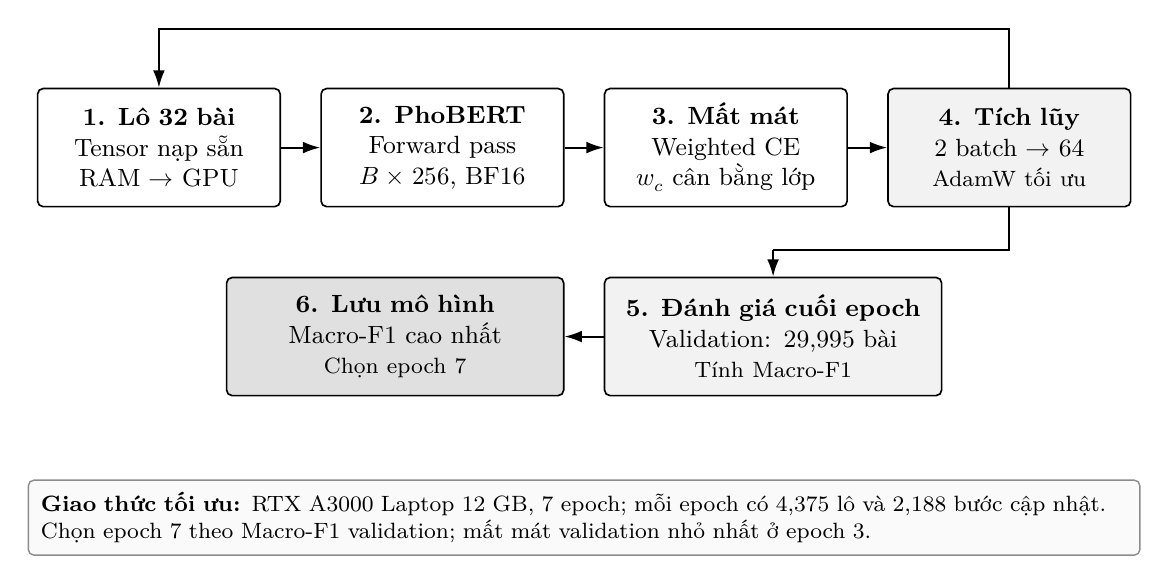
\begin{tikzpicture}
  % Row 1: Training Iteration (Left to Right, y = 1.2, width = 28mm)
  \node[arch_box, text width=28mm, minimum height=15mm] (b) at (-5.4,1.2) {
    \textbf{1. Lô 32 bài}\\
    Tensor nạp sẵn\\
    RAM $\to$ GPU
  };
  \node[arch_box, text width=28mm, minimum height=15mm] (m) at (-1.8,1.2) {
    \textbf{2. PhoBERT}\\
    Forward pass\\
    $B \times 256$, BF16
  };
  \node[arch_box, text width=28mm, minimum height=15mm] (l) at (1.8,1.2) {
    \textbf{3. Mất mát}\\
    Weighted CE\\
    $w_c$ cân bằng lớp
  };
  \node[arch_box_gray, text width=28mm, minimum height=15mm] (a) at (5.4,1.2) {
    \textbf{4. Tích lũy}\\
    \small 2 batch $\to$ 64\\
    \footnotesize AdamW tối ưu
  };

  % Row 2: Validation & Bản lưu mô hình (y = -1.2, width = 40mm, exact 9mm gap from Row 1!)
  \node[arch_box_dark, text width=40mm, minimum height=15mm] (c) at (-2.4,-1.2) {
    \textbf{6. Lưu mô hình}\\
    Macro-F1 cao nhất\\
    \footnotesize Chọn epoch 7
  };
  \node[arch_box_gray, text width=40mm, minimum height=15mm] (e) at (2.4,-1.2) {
    \textbf{5. Đánh giá cuối epoch}\\
    Validation: 29,995 bài\\
    \footnotesize Tính Macro-F1
  };

  % Forward Flow Row 1 (Clean 8mm horizontal arrows)
  \draw[arch_flow] (b) -- (m);
  \draw[arch_flow] (m) -- (l);
  \draw[arch_flow] (l) -- (a);

  % Batch Accumulation Loop: Up 8mm, left across to b.north.x, down into b.north
  \draw[arch_flow] (a.north) -- ++(0, 0.75) -| (b.north);

  % Epoch End Transition: Clean Manhattan drop at y = -0.1 (well clear of node a)
  \coordinate (epoch_turn) at (2.4, -0.1);
  \draw[arch_line] (a.south) |- (epoch_turn);
  \draw[arch_flow] (epoch_turn) -- (e.north);

  % Bản lưu mô hình selection: horizontal straight left (Clean 8mm arrow)
  \draw[arch_flow] (e) -- (c);

  % Bottom Invariant Badge (y = -3.5, generous 8mm clearance from Row 2)
  \node[arch_badge, text width=138mm] (badge) at (0,-3.5) {
    \textbf{Giao thức tối ưu:} RTX A3000 Laptop 12 GB, 7 epoch; mỗi epoch có 4,375 lô và 2,188 bước cập nhật. Chọn epoch 7 theo Macro-F1 validation; mất mát validation nhỏ nhất ở epoch 3.
  };
\end{tikzpicture}
\caption{Huấn luyện có tích lũy gradient và chọn bản lưu mô hình theo Macro-F1.}
\end{figure}
}

% -----------------------------------------------------------------------------
% 11. CalibrationDiagram: Temperature Scaling & Editorial Policy
% Node Sizes: Exactly 2 sizes:
%   - Size 1: Pipeline Stage Box (28mm x 14mm) for Row 1 (4 boxes).
%   - Size 2: Policy Routing Box (60mm x 14mm) for Row 2 (2 boxes).
% Fixed Spacing: dx = 36mm (gap = 8mm in Row 1), dy = 24mm (gap = 10mm between rows).
% -----------------------------------------------------------------------------
\newcommand{\CalibrationDiagram}{
\begin{figure}[htbp]\centering
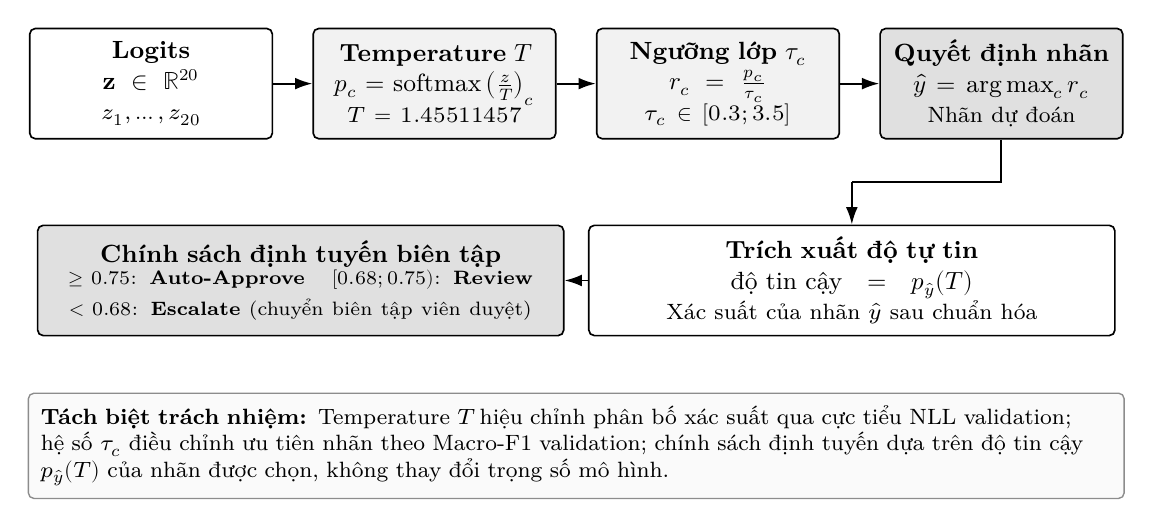
\begin{tikzpicture}
  % Stage 1: Pipeline Nodes (Horizontal, y = 1.3, width = 28mm)
  \node[arch_box, text width=28mm, minimum height=14mm] (z) at (-5.4,1.3) {
    \textbf{Logits}\\
    $\mathbf{z} \in \mathbb{R}^{20}$\\
    \footnotesize $z_1, \ldots, z_{20}$
  };
  \node[arch_box_gray, text width=28mm, minimum height=14mm] (p) at (-1.8,1.3) {
    \textbf{Temperature $T$}\\
    $p_c = \operatorname{softmax}\left(\frac{z}{T}\right)_c$\\
    \footnotesize $T = 1.45511457$
  };
  \node[arch_box_gray, text width=28mm, minimum height=14mm] (r) at (1.8,1.3) {
    \textbf{Ngưỡng lớp $\tau_c$}\\
    $r_c = \frac{p_c}{\tau_c}$\\
    \footnotesize $\tau_c \in [0.3; 3.5]$
  };
  \node[arch_box_dark, text width=28mm, minimum height=14mm] (d) at (5.4,1.3) {
    \textbf{Quyết định nhãn}\\
    $\hat{y} = \arg\max_c r_c$\\
    \footnotesize Nhãn dự đoán
  };

  % Stage 2: Policy Routing Nodes (y = -1.2, width = 64mm, height = 14mm)
  \node[arch_box, text width=64mm, minimum height=14mm] (conf) at (3.5,-1.2) {
    \textbf{Trích xuất độ tự tin}\\
    $\text{độ tin cậy} = p_{\hat{y}}(T)$\\
    \footnotesize Xác suất của nhãn $\hat{y}$ sau chuẩn hóa
  };
  \node[arch_box_dark, text width=64mm, minimum height=14mm] (route) at (-3.5,-1.2) {
    \textbf{Chính sách định tuyến biên tập}\\
    \scriptsize $\ge 0.75$: \textbf{Auto-Approve} $\quad [0.68; 0.75)$: \textbf{Review}\\
    \scriptsize $< 0.68$: \textbf{Escalate} (chuyển biên tập viên duyệt)
  };

  % Orthogonal Routing Stage 1 (Clean 8mm horizontal arrows)
  \draw[arch_flow] (z) -- (p);
  \draw[arch_flow] (p) -- (r);
  \draw[arch_flow] (r) -- (d);

  % From Decision to Confidence (Strictly Orthogonal step down at y = 0.05)
  \coordinate (cal_bus) at (3.5, 0.05);
  \draw[arch_line] (d.south) |- (cal_bus);
  \draw[arch_flow] (cal_bus) -- (conf.north);

  % From Confidence to Routing Policy (Clean 6mm horizontal arrow pointing left)
  \draw[arch_flow] (conf) -- (route);

  % Badge (y = -3.3, generous 7mm clearance from Row 2)
  \node[arch_badge, text width=136mm] (b) at (0,-3.3) {
    \textbf{Tách biệt trách nhiệm:} Temperature $T$ hiệu chỉnh phân bố xác suất qua cực tiểu NLL validation; hệ số $\tau_c$ điều chỉnh ưu tiên nhãn theo Macro-F1 validation; chính sách định tuyến dựa trên độ tin cậy $p_{\hat{y}}(T)$ của nhãn được chọn, không thay đổi trọng số mô hình.
  };
\end{tikzpicture}
\caption{Hiệu chỉnh xác suất, chọn nhãn và định tuyến biên tập là các bước riêng.}
\end{figure}
}

% -----------------------------------------------------------------------------
% 12. AppDiagram: 6-Service Microservice Architecture & Active Bundle
% Node Sizes: Exactly 1 size (36mm x 14mm) for all 6 microservices & active bundle.
% Fixed Spacing: dx = 46mm (gap = 10mm), dy = 20mm (gap = 6mm).
% -----------------------------------------------------------------------------
\newcommand{\AppDiagram}{
\begin{figure}[tbp]\centering
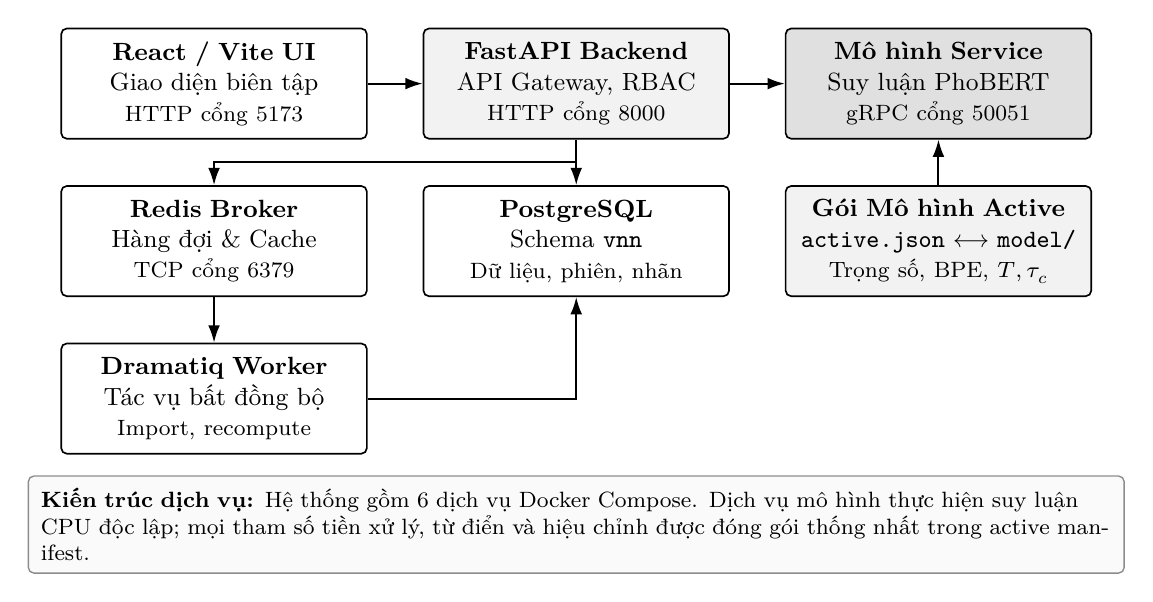
\begin{tikzpicture}
  % Column 1 (Left): Frontend & Background Queue (x = -4.6)
  \node[arch_box, text width=36mm, minimum height=14mm] (ui) at (-4.6,1.8) {
    \textbf{React / Vite UI}\\
    \small Giao diện biên tập\\
    \footnotesize HTTP cổng 5173
  };
  \node[arch_box, text width=36mm, minimum height=14mm] (redis) at (-4.6,-0.2) {
    \textbf{Redis Broker}\\
    \small Hàng đợi \& Cache\\
    \footnotesize TCP cổng 6379
  };
  \node[arch_box, text width=36mm, minimum height=14mm] (worker) at (-4.6,-2.2) {
    \textbf{Dramatiq Worker}\\
    \small Tác vụ bất đồng bộ\\
    \footnotesize Import, recompute
  };

  % Column 2 (Center): API Gateway & Database (x = 0)
  \node[arch_box_gray, text width=36mm, minimum height=14mm] (api) at (0,1.8) {
    \textbf{FastAPI Backend}\\
    \small API Gateway, RBAC\\
    \footnotesize HTTP cổng 8000
  };
  \node[arch_box, text width=36mm, minimum height=14mm] (db) at (0,-0.2) {
    \textbf{PostgreSQL}\\
    \small Schema \texttt{vnn}\\
    \footnotesize Dữ liệu, phiên, nhãn
  };

  % Column 3 (Right): Inference Service & Model Bundle (x = 4.6)
  \node[arch_box_dark, text width=36mm, minimum height=14mm] (model) at (4.6,1.8) {
    \textbf{Mô hình Service}\\
    \small Suy luận PhoBERT\\
    \footnotesize gRPC cổng 50051
  };
  \node[arch_box_gray, text width=36mm, minimum height=14mm] (artifact) at (4.6,-0.2) {
    \textbf{Gói Mô hình Active}\\
    \texttt{active.json} $\longleftrightarrow$ \texttt{model/}\\
    \footnotesize Trọng số, BPE, $T, \tau_c$
  };

  % STRICTLY ORTHOGONAL ROUTING:
  % UI -> API (10mm clean horizontal arrow)
  \draw[arch_flow] (ui) -- (api);

  % API -> Model Service (10mm clean horizontal arrow)
  \draw[arch_flow] (api) -- (model);

  % API Split Bus (y = 0.8): branch to DB and branch to Redis
  \coordinate (api_bus) at (0, 0.8);
  \draw[arch_line] (api.south) -- (api_bus);
  \draw[arch_flow] (api_bus) -- (db.north);
  \draw[arch_flow] (api_bus) -| (redis.north);

  % Redis -> Worker (Clean 6mm vertical arrow)
  \draw[arch_flow] (redis) -- (worker);

  % Worker -> DB (Strictly Orthogonal: horizontal then vertical up)
  \draw[arch_flow] (worker.east) -| (db.south);

  % Active Artifact -> Model Service (Clean 6mm vertical arrow)
  \draw[arch_flow] (artifact) -- (model);

  % Bottom Invariant Badge (y = -3.8, generous clearance from Worker)
  \node[arch_badge, text width=136mm] (badge) at (0,-3.8) {
    \textbf{Kiến trúc dịch vụ:} Hệ thống gồm 6 dịch vụ Docker Compose. Dịch vụ mô hình thực hiện suy luận CPU độc lập; mọi tham số tiền xử lý, từ điển và hiệu chỉnh được đóng gói thống nhất trong active manifest.
  };
\end{tikzpicture}
\caption{Sáu dịch vụ của ứng dụng và gói mô hình dùng cho suy luận.}
\end{figure}
}

% -----------------------------------------------------------------------------
% 13. ReviewDiagram: Editorial Loop & Provenance Tracking
% Node Sizes: Exactly 1 size (36mm x 14mm) for all 6 tracking nodes.
% Fixed Spacing: dx = 46mm (gap = 10mm), dy = 24mm (gap = 10mm).
% -----------------------------------------------------------------------------
\newcommand{\ReviewDiagram}{
\begin{figure}[tbp]\centering
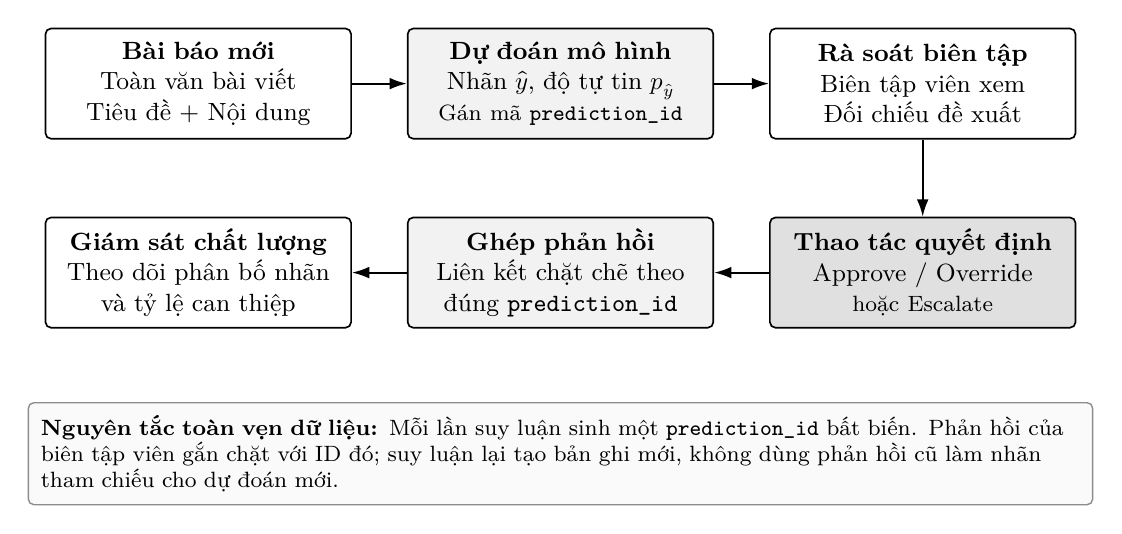
\begin{tikzpicture}
  % Upper Track: Inference & Proposal (Left to Right, y = 1.2)
  \node[arch_box, text width=36mm, minimum height=14mm] (art) at (-4.6,1.2) {
    \textbf{Bài báo mới}\\
    Toàn văn bài viết\\
    Tiêu đề + Nội dung
  };
  \node[arch_box_gray, text width=36mm, minimum height=14mm] (pred) at (0,1.2) {
    \textbf{Dự đoán mô hình}\\
    Nhãn $\hat{y}$, độ tự tin $p_{\hat{y}}$\\
    \footnotesize Gán mã \texttt{prediction\_id}
  };
  \node[arch_box, text width=36mm, minimum height=14mm] (rev) at (4.6,1.2) {
    \textbf{Rà soát biên tập}\\
    Biên tập viên xem\\
    Đối chiếu đề xuất
  };

  % Lower Track: Decision & Feedback Provenance (Right to Left, y = -1.2, exact 10mm gap!)
  \node[arch_box_dark, text width=36mm, minimum height=14mm] (dec) at (4.6,-1.2) {
    \textbf{Thao tác quyết định}\\
    Approve / Override\\
    \footnotesize hoặc Escalate
  };
  \node[arch_box_gray, text width=36mm, minimum height=14mm] (join) at (0,-1.2) {
    \textbf{Ghép phản hồi}\\
    Liên kết chặt chẽ theo\\
    đúng \texttt{prediction\_id}
  };
  \node[arch_box, text width=36mm, minimum height=14mm] (mon) at (-4.6,-1.2) {
    \textbf{Giám sát chất lượng}\\
    Theo dõi phân bố nhãn\\
    và tỷ lệ can thiệp
  };

  % Strictly Orthogonal Routing (Clean 10mm horizontal and vertical arrows)
  \draw[arch_flow] (art) -- (pred);
  \draw[arch_flow] (pred) -- (rev);
  \draw[arch_flow] (rev) -- (dec);
  \draw[arch_flow] (dec) -- (join);
  \draw[arch_flow] (join) -- (mon);

  % Invariant Badge (Spaced below join, y = -3.5, generous 9mm clearance)
  \node[arch_badge, text width=132mm] (badge) at (0,-3.5) {
    \textbf{Nguyên tắc toàn vẹn dữ liệu:} Mỗi lần suy luận sinh một \texttt{prediction\_id} bất biến. Phản hồi của biên tập viên gắn chặt với ID đó; suy luận lại tạo bản ghi mới, không dùng phản hồi cũ làm nhãn tham chiếu cho dự đoán mới.
  };
\end{tikzpicture}
\caption{Vòng phản hồi có truy vết phiên bản mô hình và lần dự đoán.}
\end{figure}
}

% -----------------------------------------------------------------------------
% 14. ActivationDiagram: Atomic Deployment & Rollback Lifecycle
% Node Sizes: Exactly 1 size (128mm x 10mm) for all 6 lifecycle stages.
% Fixed Spacing: node distance = 5.5mm.
% -----------------------------------------------------------------------------
\newcommand{\ActivationDiagram}{
\begin{figure}[tbp]\centering
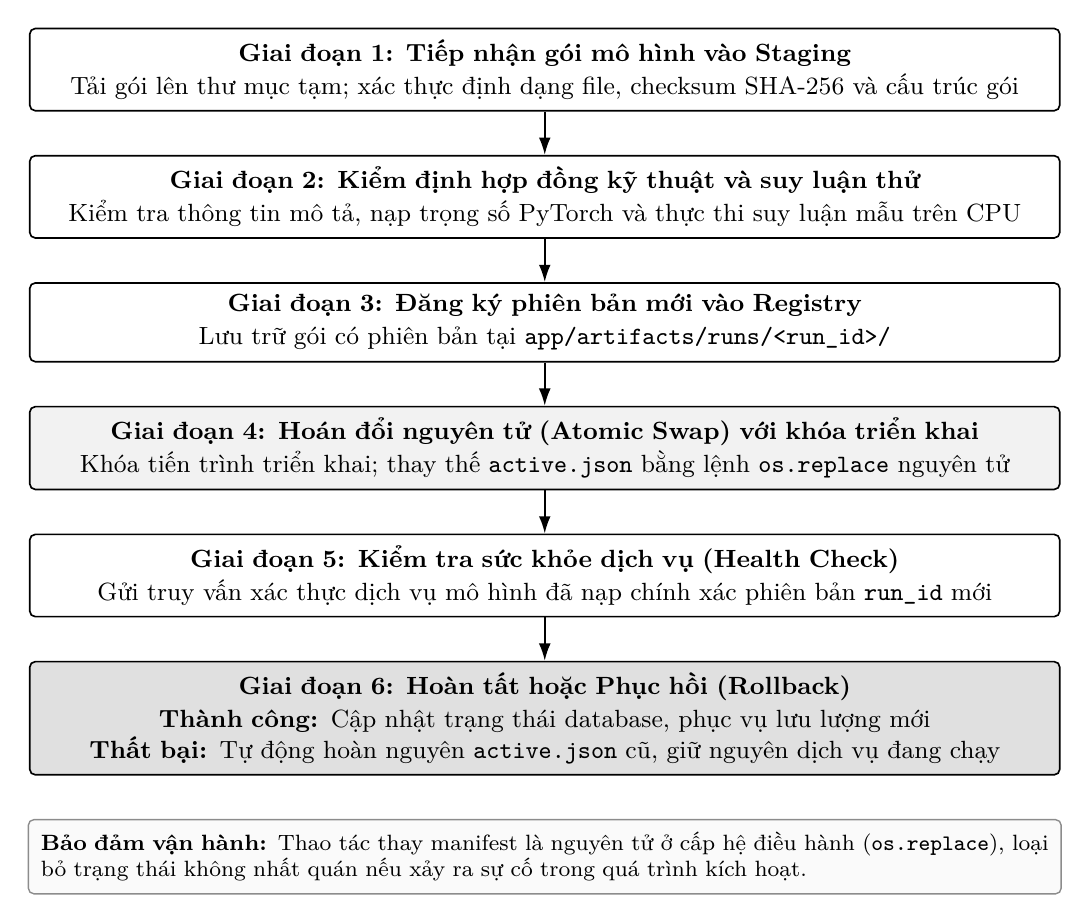
\begin{tikzpicture}[node distance=5.5mm]
  \node[arch_box, text width=128mm, minimum height=10mm] (a1) {
    \textbf{Giai đoạn 1: Tiếp nhận gói mô hình vào Staging}\\[1pt]
    Tải gói lên thư mục tạm; xác thực định dạng file, checksum SHA-256 và cấu trúc gói
  };
  \node[arch_box, text width=128mm, minimum height=10mm, below=of a1] (a2) {
    \textbf{Giai đoạn 2: Kiểm định hợp đồng kỹ thuật và suy luận thử}\\[1pt]
    Kiểm tra thông tin mô tả, nạp trọng số PyTorch và thực thi suy luận mẫu trên CPU
  };
  \node[arch_box, text width=128mm, minimum height=10mm, below=of a2] (a3) {
    \textbf{Giai đoạn 3: Đăng ký phiên bản mới vào Registry}\\[1pt]
    Lưu trữ gói có phiên bản tại \texttt{app/artifacts/runs/<run\_id>/}
  };
  \node[arch_box_gray, text width=128mm, minimum height=10mm, below=of a3] (a4) {
    \textbf{Giai đoạn 4: Hoán đổi nguyên tử (Atomic Swap) với khóa triển khai}\\[1pt]
    Khóa tiến trình triển khai; thay thế \texttt{active.json} bằng lệnh \texttt{os.replace} nguyên tử
  };
  \node[arch_box, text width=128mm, minimum height=10mm, below=of a4] (a5) {
    \textbf{Giai đoạn 5: Kiểm tra sức khỏe dịch vụ (Health Check)}\\[1pt]
    Gửi truy vấn xác thực dịch vụ mô hình đã nạp chính xác phiên bản \texttt{run\_id} mới
  };
  \node[arch_box_dark, text width=128mm, minimum height=10mm, below=of a5] (a6) {
    \textbf{Giai đoạn 6: Hoàn tất hoặc Phục hồi (Rollback)}\\[1pt]
    \textbf{Thành công:} Cập nhật trạng thái database, phục vụ lưu lượng mới\\
    \textbf{Thất bại:} Tự động hoàn nguyên \texttt{active.json} cũ, giữ nguyên dịch vụ đang chạy
  };

  % Strictly Orthogonal Straight Connections (All fixed 5.5mm vertical arrows)
  \draw[arch_flow] (a1) -- (a2);
  \draw[arch_flow] (a2) -- (a3);
  \draw[arch_flow] (a3) -- (a4);
  \draw[arch_flow] (a4) -- (a5);
  \draw[arch_flow] (a5) -- (a6);

  % Bottom Invariant Badge
  \node[arch_badge, text width=128mm, below=5.5mm of a6] (b) {
    \textbf{Bảo đảm vận hành:} Thao tác thay manifest là nguyên tử ở cấp hệ điều hành (\texttt{os.replace}), loại bỏ trạng thái không nhất quán nếu xảy ra sự cố trong quá trình kích hoạt.
  };
\end{tikzpicture}
\caption{Kiểm tra và kích hoạt một gói mô hình có kiểm soát.}
\end{figure}
}


\newcommand{\PortraitFigure}[2]{\begin{figure}[tbp]\centering
\includegraphics[width=.94\linewidth,height=.72\textheight,keepaspectratio]{#1}
\caption{#2}\end{figure}}

\newcommand{\PortraitFigureIntro}[3]{#1\PortraitFigure{#2}{#3}}

\begin{document}
\begin{titlepage}
\centering
{\large\bfseries ĐẠI HỌC QUỐC GIA TP. HỒ CHÍ MINH\\[3 pt]
TRƯỜNG ĐẠI HỌC BÁCH KHOA\\[3 pt]
KHOA KHOA HỌC VÀ KỸ THUẬT MÁY TÍNH\par}
\vspace{13 mm}

\includegraphics[width=31 mm]{assets/logos/Im0.png}\par
\vspace{14 mm}
{\Large\bfseries BÁO CÁO BÀI TẬP\par}
\vspace{6 mm}
{\large\bfseries Môn: Cách tiếp cận hiện đại trong xử lý ngôn ngữ tự nhiên\par}
\vspace{8 mm}
{\LARGE\bfseries Phân loại chủ đề tin tức tiếng Việt\\[3 pt]
với SVM, Logistic Regression, LSTM và PhoBERT\par}
\vspace{6 mm}
{\Large\bfseries Dữ liệu -- Mô hình -- Ứng dụng\par}
\vspace{6 mm}
{\large CO5087 -- Học kỳ 261 (2026--2027)\par}
\vspace{12 mm}
{\large Giảng viên: Lê Thành Sách, Nguyễn Quốc Minh\par}
\vspace{10 mm}
{\large\bfseries Thực hiện\par}
\vspace{5 mm}
{\large Đặng Nguyễn Tấn Tài \qquad 2570357\par}
\vspace{4 mm}
{\large Lớp: CH01\par}
\vfill
{\large\bfseries Thành phố Hồ Chí Minh, 10/2026\par}
\end{titlepage}
\pagenumbering{roman}
\chapter*{Tóm tắt}
\addcontentsline{toc}{chapter}{Tóm tắt}
Phân loại chuyên mục giúp tổ chức bài báo tiếng Việt và hỗ trợ điều phối biên tập. Báo cáo trình bày một quy trình gồm thu thập VietNamNet, xác minh chuyên mục trên từng bài, làm sạch corpus, biểu diễn tiếng Việt, fine-tuning PhoBERT và triển khai đề xuất nhãn có người rà soát. Bài toán sử dụng 20 lớp; nhãn mục con được quy về lớp cha trong taxonomy.

Thu thập tạo 205.463 lượt URL, tương ứng 204.280 URL duy nhất. Sau xác minh, dataset có 200.337 bài; khử trùng văn bản và loại xung đột nhãn tạo corpus 199.965 bài. Phép chia phân tầng seed 42 tạo 139.975 mẫu train, 29.995 mẫu validation và 29.995 mẫu test. Các tập không giao nhau theo URL, văn bản thô và văn bản sau tiền xử lý. Validation chọn checkpoint và fit hiệu chỉnh; test phục vụ đánh giá cuối.

PhoBERT-base-v2 được fine-tune toàn bộ encoder và đầu phân loại bằng weighted cross-entropy, trọng số tính từ train. Head--Tail giữ 127 token đầu và 127 token cuối, cộng hai token đặc biệt thành 256 vị trí. Huấn luyện chạy đủ bảy epoch trên RTX A3000 Laptop 12 GB, trong 207,17 phút; checkpoint epoch 7 đạt Macro-F1 validation 0,8723. Trên test, Accuracy đạt 91,08\% và Macro-F1 đạt 87,22\%; sau hiệu chỉnh đạt 91,13\% và 87,25\%. Temperature scaling giảm NLL từ 0,3839 xuống 0,3220 và ECE từ 0,0603 xuống 0,0251.

Chất lượng khác biệt đáng kể theo lớp. Nông thôn mới đạt F1 0,4639, trong khi Thể thao đạt 0,9880. Báo cáo phân tích mất cân bằng, giao thoa chuyên mục, giới hạn văn bản dài, chuyển đổi đúng/sai và các ví dụ truy vết được về dữ liệu. Mức tăng sau hiệu chỉnh chỉ là 13 bài đúng ròng; không đủ cơ sở kết luận vượt trội thống kê. Chưa có baseline cùng giao thức, thực nghiệm nhiều seed hay kiểm tra theo thời gian và ngoài miền.

Ứng dụng sáu dịch vụ dùng cùng trọng số, tokenizer, mapping và hiệu chỉnh của notebook. Các chức năng nhập bài, dự đoán, rà soát, quản lý ngưỡng, registry và monitoring được kiểm tra với dữ liệu minh họa từ corpus. Chỉ số offline, mô phỏng định tuyến và monitoring từ phản hồi được trình bày theo đúng phạm vi, tránh coi bộ ví dụ giao diện là một tập kiểm tra độc lập.

\chapter*{Danh mục thuật ngữ}
\addcontentsline{toc}{chapter}{Danh mục thuật ngữ}
\begin{longtable}{p{32mm}p{118mm}}
\toprule Thuật ngữ & Ý nghĩa trong báo cáo\\\midrule
Corpus & Tập bài báo, nhãn chuyên mục và metadata nguồn.\\
Phân đoạn từ & Xác định từ tiếng Việt gồm một hoặc nhiều âm tiết.\\
BPE & Mã hóa từ thành các đơn vị subword của tokenizer.\\
Head--Tail & Giữ đầu và cuối chuỗi token khi vượt giới hạn đầu vào.\\
Fine-tuning & Cập nhật mô hình tiền huấn luyện cho tác vụ chuyên mục.\\
Validation & Chọn checkpoint và xác định tham số hiệu chỉnh.\\
Test độc lập & Tập đánh giá cuối không tham gia chọn hoặc fit tham số.\\
Macro-F1 & Trung bình F1 của 20 lớp, mỗi lớp đóng góp bằng nhau.\\
Weighted-F1 & Trung bình F1 theo số mẫu của từng lớp.\\
NLL & Mất mát log xác suất nhãn tham chiếu, không trọng số lớp.\\
ECE & Sai lệch confidence và tỷ lệ đúng theo 15 khoảng xác suất.\\
Temperature & Tham số dương $T$ chia logits trước softmax.\\
Hệ số lớp & $\tau_c$ trong điểm quyết định $p_c(T)/\tau_c$.\\
Confidence & Xác suất của nhãn được chọn bởi quy tắc quyết định.\\
Routing & Phân luồng auto-approve, review hoặc escalate.\\
Artifact & Trọng số, tokenizer, mapping và cấu hình suy luận.\\
Prediction ID & Khóa lần suy luận để gắn phản hồi đúng kết quả.\\
\bottomrule\end{longtable}

\tableofcontents
\listoffigures
\listoftables
\clearpage
\pagenumbering{arabic}
\chapter{Bài toán và thiết kế đánh giá}\label{chap:problem}
\FloatBarrier
\section{Bối cảnh và phát biểu bài toán}
Mỗi bài báo VietNamNet được tổ chức theo một chuyên mục biên tập, nhưng nội dung có thể giao thoa nhiều lĩnh vực. Bài toán đặt ra là dự đoán một chuyên mục chính từ tiêu đề và nội dung, trong khi nhãn tham chiếu phản ánh taxonomy của tòa soạn thay vì một hệ phân loại chủ đề phổ quát. Các khó khăn gồm phân đoạn từ tiếng Việt, độ dài bài báo, chênh lệch số mẫu giữa các lớp và ranh giới nhãn không hoàn toàn tách biệt. Chất lượng nguồn nhãn và tính nhất quán của phép chia dữ liệu vì vậy có vai trò quan trọng bên cạnh lựa chọn bộ phân loại.

Với $x_i=(t_i,b_i)$ gồm tiêu đề và nội dung, $y_i\in\mathcal C$, $|\mathcal C|=20$, corpus giám sát là
\begin{equation}\mathcal D=\{(x_i,y_i)\}_{i=1}^{199\,965}.\end{equation}
Phương pháp $m$ biến đổi văn bản bằng $\phi_m$, sinh điểm với mô hình $f_{\theta_m}$ và chọn nhãn:
\begin{equation}
z_i^{(m)}=f_{\theta_m}(\phi_m(x_i)),\qquad
\hat y_i^{(m)}=\arg\max_{c\in\mathcal C}z_{i,c}^{(m)}.
\end{equation}
Argmax là giao thức đối chứng chính. Riêng PhoBERT có thêm quy tắc quyết định theo lớp để phục vụ ứng dụng, được đánh giá tách biệt. URL và breadcrumb dùng xác minh nguồn nhãn, không trở thành đặc trưng của bộ phân loại. Top-$k$ là các ứng viên cạnh tranh, không phải một tập nhãn cùng đúng: tác vụ là đa lớp đơn nhãn.

Một bài về sinh kế vùng dân tộc có thể đồng thời chứa du lịch, văn hóa và chính sách. Vì thế, sai số được hiểu là không khớp chuyên mục tham chiếu, chưa mặc nhiên là sai theo mọi cách diễn giải nội dung. Mô hình không kiểm chứng thông tin trong bài và không có bộ phát hiện chắc chắn văn bản ngoài taxonomy.

\FloatBarrier
\section{Mục tiêu nghiên cứu và phạm vi}
SVM, Logistic Regression, BiLSTM và PhoBERT được lựa chọn để khảo sát ba họ biểu diễn: đặc trưng từ vựng, embedding chuỗi và biểu diễn ngữ cảnh tiền huấn luyện. Báo cáo trả lời ba câu hỏi:
\begin{enumerate}[label=\textbf{RQ\arabic*:},leftmargin=17mm]
\item Trên cùng corpus VietNamNet và taxonomy 20 chuyên mục, chất lượng phân loại của bốn phương pháp khác nhau như thế nào?
\item Khác biệt chất lượng có tương xứng với thời gian huấn luyện, bộ nhớ và chi phí suy luận của từng hướng tiếp cận không?
\item Các phương pháp khác nhau thế nào ở chuyên mục ít mẫu hoặc có nội dung giao thoa?
\end{enumerate}
Notebook dữ liệu tạo đầu vào chung; bốn notebook huấn luyện tự chứa quy trình tạo biểu diễn, chọn cấu hình, đánh giá và xuất artifact. LSTM được thực thi bằng biến thể hai chiều BiLSTM, với embedding học từ đầu. Các gói đối chứng phục vụ đánh giá offline; ứng dụng minh họa dùng PhoBERT để đề xuất nhãn, hỗ trợ rà soát và lưu phản hồi (Phụ lục~\ref{app:application}).

So sánh xem xét hiệu quả toàn bộ pipeline trong một điều kiện thực nghiệm cụ thể. Nó chưa tách riêng đóng góp của kiến trúc, pretraining, stopword, lặp tiêu đề hay vùng văn bản được giữ. Phân tích lớp hiếm và độ tin cậy xác suất bổ sung cho điểm tổng, nhưng không thay thế đánh giá ngoài nguồn hoặc nhiều lần train.


Nhãn cuối là một quyết định của bài toán đơn nhãn, còn confidence phục vụ đánh giá mức chắc chắn trong điều kiện taxonomy. Một bài ngoài miền vẫn có thể được gán nhãn cao điểm do bộ phân loại chỉ có 20 lựa chọn; không coi tổng xác suất bằng 1 như bằng chứng đầu vào hợp lệ. Vì thế, ba câu hỏi nghiên cứu không chỉ hỏi model nào có điểm cao nhất, mà còn hỏi lỗi rơi vào đâu và số đo nào có thể hỗ trợ sử dụng kết quả.

Phạm vi ứng dụng là vòng rà soát có người quyết định, không gồm tự sinh bài hoặc tự cập nhật trọng số từ feedback. Bằng chứng giao diện giải thích cách kết quả NLP được dùng; nó không được cộng vào test hoặc dùng chứng minh tổng quát hóa. Sự tách biệt giữa thực nghiệm và minh họa giúp cùng một chỉ số không bị gán hai ý nghĩa khác nhau.

\FloatBarrier
\section{Giao thức dữ liệu và tiêu chí đánh giá}
Khử trùng diễn ra trước chia tập. Phép chia phân tầng 70/15/15, seed 42 tạo train 139.975 bài và hai tập validation, test, mỗi tập 29.995 bài. Bốn pipeline có cùng chỉ số chia, URL và nhãn test theo thứ tự. Train dùng cập nhật trọng số, tính class weights và fit vocabulary/IDF; validation chọn cấu hình, checkpoint và tham số hiệu chỉnh; test chỉ đánh giá cuối sau khi các lựa chọn đã cố định.
\SplitDiagram
Macro-F1 là tiêu chí lựa chọn để mỗi lớp đóng góp ngang nhau; Accuracy và Weighted-F1 bổ sung góc nhìn theo số bài. Kết quả theo lớp, confusion matrix và lỗi truy vết chỉ ra nơi chất lượng suy giảm. Chương~\ref{chap:experiments} đánh giá riêng chất lượng nhãn, xác suất và chi phí, tránh lấy một chỉ số thay thế tất cả yêu cầu.

Validation được dùng cho cả lựa chọn model và hiệu chỉnh. Sự dùng lại này tạo phụ thuộc vào tập validation, dù test không tham gia fit. Một seed hỗ trợ tái tạo phép chia trong snapshot, chưa đo biến thiên huấn luyện. Chín đối chiếu giữa các tập theo URL, văn bản thô và văn bản chuẩn hóa không phát hiện giao nhau chính xác; phạm vi kiểm tra chưa bao gồm gần trùng hoặc bài cùng sự kiện.

Bốn pipeline được đánh giá trên cùng corpus sau khử trùng và cùng tập test; các phép học biểu diễn riêng chỉ dùng train. Chương tiếp theo xem xét bằng chứng nghiên cứu làm cơ sở lựa chọn các phương pháp.

\chapter{Tổng quan nghiên cứu và lựa chọn phương pháp}
\label{chap:related}
\FloatBarrier
\section{Các hướng biểu diễn trong phân loại văn bản}
Một hệ thống phân loại văn bản kết hợp tiền xử lý, biểu diễn đầu vào, bộ phân loại và giao thức đánh giá. Khảo sát của Kowsari và cộng sự tổ chức các phương pháp theo những thành phần này \citep{kowsari2019}. Cách nhìn đó giúp phân biệt ba hướng: đặc trưng từ vựng như BoW/TF--IDF; vector biểu diễn từ kết hợp mạng xử lý chuỗi; biểu diễn theo ngữ cảnh từ mô hình ngôn ngữ tiền huấn luyện. Khác biệt giữa các hướng nằm cả ở thông tin được giữ trong đầu vào lẫn tri thức học được, không chỉ ở tên thuật toán.

Phân loại tin tức tiếng Việt có nền tảng thực nghiệm trước thời kỳ Transformer. Hoang và cộng sự khảo sát BoW, lựa chọn đặc trưng và mô hình ngôn ngữ n-gram trên tập dữ liệu tin tức hai cấp nhãn \citep{hoang2007}. Công trình tại FAIR'9 sử dụng từ lõi và xác suất có điều kiện với Naive Bayes trên 220 văn bản, sáu chủ đề \citep{linh2016}. Đây là ví dụ về lựa chọn tín hiệu đại diện cho chuyên mục; mô hình từ lõi không đồng nhất với LDA, và quy mô thử nghiệm nhỏ chưa đại diện bài toán hiện tại.

Khoảng trắng tiếng Việt thường phân cách âm tiết, nên đơn vị đếm không mặc nhiên là từ. Khảo sát của Nguyễn Chí Hiếu nhấn mạnh vai trò biểu diễn và phân đoạn từ trong phân loại tiếng Việt \citep{hieu2022}. VnCoreNLP là một công trình tiêu biểu về công cụ phân đoạn và phân tích ngôn ngữ \citep{vncorenlp2018}. Nghiên cứu này dùng PyVi để phân đoạn từ; VnCoreNLP được nêu như một công trình liên quan để làm rõ bối cảnh lựa chọn công cụ. Các khảo sát giúp tổ chức phương pháp nhưng không cung cấp một phép so sánh trực tiếp bốn mô hình trên tập dữ liệu VietNamNet này.

\FloatBarrier
\section{Phương pháp tuyến tính trên đặc trưng từ vựng}
TF--IDF tạo vector thưa, có số chiều phụ thuộc từ vựng và n-gram. SVM tuyến tính học ranh giới có biên giữa các lớp trong không gian đó; Logistic Regression (LR) học điểm tuyến tính bằng mục tiêu mất mát logarit. Cả hai khai thác đồng thời nhiều đặc trưng và điều chuẩn, không cần huấn luyện encoder ngôn ngữ lớn. TF--IDF không mô hình hóa đầy đủ thứ tự dài, nhưng n-gram vẫn giữ được một phần ngữ cảnh cục bộ \citep{kowsari2019}.

Trần Cao Đệ và Phạm Nguyên Khang dùng 7,842 bài thuộc 10 chủ đề từ báo điện tử, gồm VietNamNet, với 5,000 bài train và 2,842 bài test. TF--IDF kết hợp SVD và SVM đạt F1 trung bình được báo cáo là 91.0\%, so với 84.1\% của cây quyết định \citep{de2012}. Kết quả cho thấy biểu diễn và giảm chiều có thể ảnh hưởng chất lượng. Tuy nhiên, SVD được mô tả trên ma trận toàn tập dữ liệu trước huấn luyện bộ phân loại; giao thức đó chưa bảo đảm một đánh giá quy nạp chỉ học biến đổi từ train. Không suy ra SVD bắt buộc cho SVM, và không sao chép cách học tham số này vào đối chứng mới.

Trên VNNews-01 gồm 37,500 bài, 25 lớp từ hơn 30 website, Duong và Truong Hoang đánh giá bằng trung bình F-measure qua kiểm định chéo năm phần dữ liệu. SVM kernel RBF đạt 0.749; LR multinomial đạt 0.734 \citep{duong2019}. Giá trị 0.749 thuộc RBF, không phải LinearSVC; nguồn cũng chưa xác định rõ cách tổng hợp F-measure theo lớp. Đây là bằng chứng cho tính khả thi của cả SVM và LR, không phải một mức Macro-F1 có thể đối chiếu với bài tập lớn.

LR có lý do lựa chọn riêng, không chỉ là phương án thay thế khi không dùng SVM. Trong nghiên cứu của Nguyen Thi Hien và cộng sự, LR với TF--IDF đạt Accuracy 92.77\% ở Level 1 \citep{hien2024}; trên BN-VN3S, LR đạt Macro-F1 91.36\%, còn LinearSVC đạt 92.33\% \citep{chau2026}. Hai bộ phân loại cùng biểu diễn nhưng khác mục tiêu tối ưu tạo đối chứng để kiểm tra liệu tín hiệu từ vựng đã giải thích phần lớn nhãn hay chưa. Lựa chọn tuyến tính cũng phù hợp khảo sát tập dữ liệu lớn, song chi phí thực tế vẫn phải đo trên cùng phần cứng.

\FloatBarrier
\section{Mạng hồi tiếp và vector biểu diễn từ}
Vector biểu diễn từ biểu diễn token bằng vector đặc, còn LSTM tích lũy trạng thái theo thứ tự chuỗi. Hướng này có thể học quan hệ vượt một n-gram cố định mà không dùng encoder Transformer tiền huấn luyện \citep{kowsari2019}. Vector biểu diễn từ tĩnh không tự trở thành biểu diễn theo ngữ cảnh; ngữ cảnh được hình thành qua mạng xử lý chuỗi. Trạng thái phụ thuộc bước trước làm hạn chế song song hóa theo chiều thời gian khi chuỗi dài. Chiều dài đầu vào, chất lượng phân đoạn, nguồn vector biểu diễn từ và khả năng học từ ít gặp đều ảnh hưởng kết quả.

Nguyen Thi Hien và cộng sự khảo sát LR, cây quyết định, SVM, LSTM và CNN trên hai cấp nhãn 10/27 của tập dữ liệu tin tức. Ở Level 1, LSTM với BoW đạt Accuracy 94.52\%; với TF--IDF, LSTM đạt 93.75\% và SVM đạt 93.60\% \citep{hien2024}. Các giá trị hỗ trợ nghiên cứu LSTM trên tiếng Việt nhưng chưa tách tác động kiến trúc khỏi biểu diễn. Nguồn chưa giải thích đủ việc chuyển đặc trưng BoW/TF--IDF và SVD thành trục tuần tự của LSTM. Vì vậy, thiết kế khảo sát ở đây dùng chuỗi token có thứ tự và vector biểu diễn từ, không coi các chiều TF--IDF là vị trí từ.

UIT-ViON đối chiếu LSTM với nhiều vector biểu diễn từ cùng LR, TextCNN và PhoBERT trên tiêu đề tin \citep{tran2021}. Kết quả này bổ sung bằng chứng ở đầu vào ngắn; không chứng minh cùng cấu hình phù hợp bài dài. Một hướng LSTM--CNN cũng được thực nghiệm trên cảm xúc tiếng Việt \citep{vo2017}, nhưng tác vụ cảm xúc và kiến trúc lai không phải benchmark cho LSTM phân loại chuyên mục. Tương tự, BiGRU trong BN-VN3S là bằng chứng về họ mạng hồi tiếp, không phải kết quả của LSTM \citep{chau2026}.

\FloatBarrier
\section{PhoBERT và mô hình tiền huấn luyện}
PhoBERT phát triển mô hình ngôn ngữ tiền huấn luyện riêng cho tiếng Việt theo hướng RoBERTa, kết hợp phân đoạn từ và BPE trước học biểu diễn ngữ cảnh \citep{phobert}. Fine-tuning tận dụng tham số đã học trên tập dữ liệu lớn cho tác vụ có giám sát, đi kèm yêu cầu bộ nhớ và giới hạn chiều dài đầu vào. Bài PhoBERT gốc đánh giá POS, parsing, NER và NLI, không trực tiếp cung cấp kết quả phân loại chuyên mục của bài tập lớn. Bản lưu mô hình \texttt{phobert-base-v2} có thông tin riêng từ tài liệu mô hình và config; chương~\ref{chap:model} trình bày cấu hình thực thi.

UIT-ViON gồm 260,000 tiêu đề, 13 chủ đề từ sáu nguồn, chia train/validation/test theo 80/10/10. PhoBERT đạt F1-score 80.62\%, cao nhất trong bảng kết quả của nguồn \citep{tran2021}. Tuy nhiên, bài gọi tác vụ đa nhãn ở Abstract/Conclusion và mô tả sigmoid/BCE, trong khi các phần khác dùng cách diễn đạt đa lớp và cấu hình softmax. Mục đánh giá gọi F1 là macro-averaged. Sự không nhất quán về giao thức nhãn cần được giữ trong diễn giải; không coi đây là đối chứng đồng nhất với 20 lớp đơn nhãn. Tiêu đề cũng không chứa toàn bộ nội dung và không có vấn đề cắt bài dài như tập dữ liệu hiện tại.

BN-VN3S của Chau và cộng sự cung cấp 946,696 bài từ VietNamNet, VnExpress và Dân Trí, với 10 chủ đề. Phép chia phân tầng 80/10/10 được dùng chung, các kết quả lấy trung bình ba seed. Macro-F1 của BiGRU, LinearSVC và PhoBERT lần lượt là 92.42\%, 92.33\% và 87.98\% \citep{chau2026}. Transformer được fine-tune với cơ chế cửa sổ trượt 256 token rồi tổng hợp ở cấp bài. Thứ hạng trong thiết lập này bác bỏ giả định Transformer mặc nhiên tốt nhất; nó không chứng minh SVM hay mạng hồi tiếp luôn tốt hơn PhoBERT.

BN-VN3S còn đánh giá thay đổi theo thời gian và để riêng một nguồn báo làm test. Những thiết lập đó đặt câu hỏi tổng quát hóa khác với chia ngẫu nhiên cùng phân phối \citep{chau2026}. Tập dữ liệu có VietNamNet không có nghĩa hệ thống chuyên mục, bản dữ liệu hay nhãn trùng bài tập lớn. Bản nghiên cứu của Kiệt và Lang cung cấp bằng chứng bổ trợ: sau lọc còn 162,580 bài dài 100--300 từ, F1 của LR/SVM/BiLSTM--CNN/PhoBERT là 0.894/0.896/0.888/0.907 \citep{kietlang}. Nguồn chưa xác định rõ cách tổng hợp F1 và chưa xác minh được nơi công bố. Không đổi các giá trị thành Macro-F1; mô hình lai và tập dữ liệu lọc độ dài cũng khác LSTM và Head--Tail của thiết kế hiện tại.

\FloatBarrier
\section{Tổng hợp các công trình và cơ sở so sánh bốn phương pháp}
Bảng~\ref{tab:related} tập trung các nghiên cứu tin tức. Các giá trị chỉ có ý nghĩa trong điều kiện từng hàng, không tạo thứ hạng liên nghiên cứu. Khác nguồn, số lớp, đơn vị đầu vào, cách lọc, phép chia và metric đều có thể thay đổi độ khó. Accuracy không thay Macro-F1; F1 chưa rõ cách tổng hợp không được tự gán thành Macro-F1 hay Weighted-F1.

\begingroup
\small
\setlength{\tabcolsep}{3pt}
\begin{longtable}{@{}>{\raggedright\arraybackslash}p{0.17\linewidth}>{\raggedright\arraybackslash}p{0.24\linewidth}>{\raggedright\arraybackslash}p{0.20\linewidth}>{\raggedright\arraybackslash}p{\dimexpr0.39\linewidth-18pt\relax}@{}}
\caption{Nghiên cứu phân loại tin tức tiếng Việt và điều kiện diễn giải; số liệu thuộc từng nguồn, không phải benchmark chung.}\label{tab:related}\\
\toprule
Nghiên cứu & Dữ liệu và giao thức & Phương pháp chính & Phát hiện và giới hạn\\\midrule
\endfirsthead
\multicolumn{4}{l}{\tablename\ \thetable\ (tiếp theo)}\\
\toprule Nghiên cứu & Dữ liệu và giao thức & Phương pháp chính & Phát hiện và giới hạn\\\midrule
\endhead
\bottomrule\endfoot
Hoang và cộng sự (2007) \citep{hoang2007} & Tin tức đa nguồn; hai cấp 10/27 nhãn; train/test riêng. & BoW, chọn đặc trưng, SVM và mô hình n-gram. & Biểu diễn ảnh hưởng chất lượng; hệ thống chuyên mục và giao thức lịch sử khác tập dữ liệu hiện tại.\\[4pt]
Trần Cao Đệ, Phạm Nguyên Khang (2012) \citep{de2012} & 7,842 bài, 10 chủ đề; train 5,000, test 2,842. & TF--IDF, SVD, SVM; cây quyết định. & F1 trung bình báo cáo 91.0\% và 84.1\%; SVD trên toàn tập dữ liệu cần lưu ý khi tái hiện.\\[4pt]
Duong, Truong Hoang (2019) \citep{duong2019} & VNNews-01: 37,500 bài, 25 lớp; kiểm định chéo năm phần dữ liệu. & TF--IDF; SVM, LR và các bộ phân loại khác. & F-measure: RBF SVM 0.749, LR 0.734; chưa rõ tổng hợp theo lớp.\\[4pt]
Tran và cộng sự (2021) \citep{tran2021} & UIT-ViON: 260,000 tiêu đề, 13 chủ đề; 80/10/10. & TF--IDF + LR; vector biểu diễn từ + CNN/LSTM; PhoBERT. & PhoBERT F1 80.62\%; nguồn mô tả đa nhãn nhưng giao thức chưa nhất quán; đầu vào ngắn.\\[4pt]
Nguyen Thi Hien và cộng sự (2024) \citep{hien2024} & Tập dữ liệu tin tức hai cấp 10/27 nhãn; kết quả nêu ở Level 1. & BoW/TF--IDF; LR, SVM, LSTM, CNN. & Accuracy: LSTM--BoW 94.52\%, SVM--TF--IDF 93.60\%; đầu vào tuần tự cần làm rõ.\\[4pt]
Kiệt, Lang (s.d.) \citep{kietlang} & 162,580 bài, 9 lớp; lọc 100--300 từ; train/test khoảng 80/20. & TF--IDF + LR/SVM; BiLSTM--CNN; PhoBERT. & F1: 0.894/0.896/0.888/0.907; chưa rõ tổng hợp F1 và venue; bằng chứng bổ trợ.\\[4pt]
Chau và cộng sự (2026) \citep{chau2026} & BN-VN3S: 946,696 bài, 10 chủ đề; 80/10/10, ba seed; thêm test nguồn/thời gian. & TF--IDF + LR/LinearSVC; BiGRU; PhoBERT và các mô hình khác. & Macro-F1: BiGRU 92.42\%, LinearSVC 92.33\%, PhoBERT 87.98\%; phụ thuộc cấu hình và dữ liệu.\\
\end{longtable}
\endgroup

\subsection{Lựa chọn ba họ biểu diễn}
SVM và LR là hai đối chứng tuyến tính dùng TF--IDF: một hướng tối ưu biên phân lớp, một hướng tối ưu mất mát logarit. Giữ cùng cách biểu diễn giúp khảo sát ảnh hưởng mục tiêu học. LSTM khảo sát biểu diễn chuỗi và thứ tự token; PhoBERT khảo sát biểu diễn ngữ cảnh có tiền huấn luyện tiếng Việt. Bốn lựa chọn bao phủ ba họ biểu diễn có bằng chứng liên quan, với các yêu cầu tài nguyên và cách dùng thông tin khác nhau.

\MethodFamiliesDiagram

Để so sánh công bằng, các phương pháp cần dùng cùng tập dữ liệu sau làm sạch, hệ thống chuyên mục 20 lớp và cùng các tập huấn luyện, xác thực, kiểm tra. Từ vựng, IDF và các biến đổi học từ dữ liệu chỉ học từ tập huấn luyện; validation chọn siêu tham số, test đánh giá cuối. Macro-F1 là tiêu chí chính, cùng Accuracy, Weighted-F1 và precision/recall theo lớp. Thời gian, bộ nhớ và tốc độ suy luận cần đo với môi trường, batch và phạm vi công việc được công bố. Khác biệt về tiền huấn luyện, vector biểu diễn từ và phần văn bản được giữ phải được nêu rõ: đây là so sánh các quy trình phân loại thực tế, chưa phải ablation chỉ thay kiến trúc.

Tập dữ liệu hiện tại có 20 chuyên mục của một tòa soạn, lớp ít mẫu và ranh giới giao thoa; số bài giữa các lớp chênh lệch đáng kể. Những đặc điểm này khác hệ thống chuyên mục rộng 10/13 chủ đề, tiêu đề ngắn hoặc tập dữ liệu đã lọc độ dài trong nghiên cứu trước. Vì vậy, lựa chọn mô hình cần được kiểm chứng trên dữ liệu của bài tập lớn, đặc biệt ở nhóm Nông thôn mới, Nội dung chuyên đề và các chuyên mục dân tộc, thay vì suy ra từ một F1 tổng thể bên ngoài.

\subsection{Giới hạn của nghiên cứu liên quan và nguyên tắc đối chứng}
Nghiên cứu trước cung cấp căn cứ lựa chọn, còn các notebook SVM, LR, BiLSTM và PhoBERT tạo bằng chứng đối chứng trên tập dữ liệu hiện tại. Chương~\ref{chap:experiments} đối chiếu các quy trình phân loại được lựa chọn trên cùng tập test; validation chỉ được dùng để chọn cấu hình, bản lưu mô hình và tham số hiệu chỉnh. Bằng chứng bên ngoài không xác định trước thứ hạng trên dữ liệu của bài tập lớn; một kết quả cao nhất cũng không chứng minh ưu thế trên mọi tập dữ liệu, seed hay điều kiện triển khai. Ứng dụng dùng gói PhoBERT được kiểm chứng độc lập với phạm vi đối chứng offline.

Một phép so sánh có ý nghĩa trước hết cần đầu vào và nhãn đáng tin cậy. Chương~\ref{chap:data} xác định nguồn tin, quy tắc nhãn cha--con, chuyển chuyên mục ở cấp bài, loại bỏ bài trùng lặp và giới hạn tập dữ liệu. Đây là cơ sở chung cho các phương pháp, trước khi xét biểu diễn và tối ưu riêng của bốn quy trình phân loại.

\chapter{Tập dữ liệu VietNamNet và tiền xử lý tiếng Việt}\label{chap:data}
\FloatBarrier
\section{Thu thập, xác minh chuyên mục và tạo tập dữ liệu}
Tập dữ liệu gồm bài VietNamNet trong 20 chuyên mục được chọn. Notebook thu thập trên tối đa 500 trang danh sách cho mỗi chuyên mục, rồi tải nội dung bằng 32 luồng xử lý song song; số 500 là giới hạn trang, không phải số bài. Một trang chứa nhiều URL, một URL có thể xuất hiện tại nhiều chuyên mục và chuyên mục ngắn kết thúc khi hết dữ liệu hợp lệ. Phạm vi này không bao phủ toàn bộ kho tin của website.

Trang danh sách dùng để phát hiện bài. Nhãn được kiểm tra trên chính trang bài, dựa vào đường dẫn chuyên mục và breadcrumb, tức chuỗi liên kết thể hiện vị trí của bài trong các mục cha--con. Tiêu đề, nội dung, URL chính thức (canonical) và bằng chứng chuyên mục được lấy cùng lượt tải HTML. Nếu thuộc chuyên mục nguồn, bài được giữ; nếu bằng chứng chỉ tới một lớp khác trong hệ thống chuyên mục, cả URL và nội dung chuyển về lớp đó. Bài ngoài hệ thống chuyên mục bị loại; lỗi tải, thiếu nội dung hoặc bằng chứng chưa đủ được thử tối đa ba lượt trước khi loại.

Mỗi nhãn có mã file ổn định. Đường dẫn Công nghiệp hỗ trợ là \texttt{hop-tac/}\allowbreak\texttt{cong-nghiep-ho-tro}, còn nhãn và tên Parquet là Công nghiệp hỗ trợ; phần đường dẫn đứng trước không tạo lớp mới. Sắc màu Việt Nam là mục con của Dân tộc -- Tôn giáo và quy về lớp cha. Không dùng mô hình đang huấn luyện để tự gán nhãn cho tập dữ liệu của chính nó: nhãn được xác định từ bằng chứng xuất bản, không từ từ khóa nội dung.

\DataTable{tables/cleaning_counts.tex}{Lượt URL, URL duy nhất và dòng văn bản là các đơn vị đếm khác nhau.}
205,463 lượt phát hiện tạo 204,280 URL duy nhất. Số bài giữ nhãn nguồn cộng số bài chuyển bằng 200,337; các nhánh còn lại gồm 3,866 bài ngoài hệ thống chuyên mục, 76 trường hợp không đạt sau ba lượt và một yêu cầu tải chuyển về địa chỉ chính thức đã có:
\begin{equation}204{,}280=199{,}463+874+3{,}866+76+1.\end{equation}
874 là số bài chuyển tính theo URL duy nhất. Thông tin mô tả quan hệ nguồn--đích có thể tính một bài ở nhiều nguồn; vì vậy, tổng ô ngoài đường chéo không thay được số bài chuyển. Trong đó có 225 quan hệ Dân tộc -- Tôn giáo tới Chính trị và 204 quan hệ Tuần Việt Nam tới Nội dung chuyên đề.
\CorpusAuditDiagram
Bản dữ liệu lưu bốn tệp JSON: raw chứa URL phát hiện, removed chứa URL bị loại hoặc gộp, meta chứa thông tin kiểm chứng, clean chứa URL theo nhãn cuối. Các tệp liên kết với nhau để truy vết một bài từ lúc phát hiện đến khi xác định nhãn cuối. Parquet giữ URL, tiêu đề, nội dung, nhãn và bằng chứng xác minh. Kiểm tra cấu trúc tệp và mã băm (hash) giúp xác nhận dữ liệu nhất quán với các quy tắc đã đặt ra. Mã băm nhận diện nội dung tệp, không chứng minh mọi nhãn đều đúng về ngữ nghĩa hoặc đã được chuyên gia gán thủ công.



\subsection{Thuật toán xác định chuyên mục cấp bài}
Chuyên mục được nhận diện theo đường dẫn (route) đã khai báo, xét đường dẫn dài trước để không chọn nhầm lớp cha khi có đường dẫn cụ thể hơn. URL được chuẩn hóa về tên miền VietNamNet hợp lệ; không lấy đường dẫn trùng tên ở một tên miền khác làm bằng chứng hệ thống chuyên mục. Canonical về cổng giảm nghèo riêng được xác định ngoài phạm vi, không ghép nhầm vào lớp chỉ vì có nội dung về vùng dân tộc.

\begin{enumerate}[leftmargin=1.6em]
\item Đọc dữ liệu có cấu trúc JSON-LD trong mã HTML trước khi trích xuất văn bản. Từ trường BreadcrumbList, thu các chuỗi chuyên mục, sắp theo thuộc tính position và đối chiếu đường dẫn với danh sách chuyên mục đã khai báo.
\item Đọc liên kết trực tiếp của breadcrumb hiển thị tại bài. Không lấy nhãn từ danh sách xổ xuống chứa toàn bộ chuyên mục của website, vì danh sách này không mô tả riêng bài đang tải.
\item Với chuỗi có thông tin ngoài mục Trang chủ (Home), lấy mục cuối khớp đường dẫn. Nếu các nguồn breadcrumb đưa ra chuyên mục khác nhau, đánh dấu chưa giải quyết để thử lại; không chọn tùy ý nguồn dễ khớp nhất.
\item Chỉ khi không có breadcrumb hữu ích, dùng trường articleSection của dữ liệu có cấu trúc nếu các tên mục quy về duy nhất một nhãn trong hệ thống chuyên mục. Trường hợp thiếu hoặc mâu thuẫn bằng chứng không được gán nhãn theo tiêu đề.
\end{enumerate}
Ba trạng thái kiểm chứng là accepted (chấp nhận), outside (ngoài phạm vi) và unresolved (chưa đủ căn cứ). Accepted cung cấp nhãn và đường dẫn bằng chứng; outside chỉ bài hợp lệ nhưng không có chuyên mục trong phạm vi; unresolved chỉ tình huống chưa đủ tin cậy để xác minh. Tải lại có thể giải quyết lỗi mạng hoặc bổ sung thông tin mô tả còn thiếu, nhưng không biến một mục ngoài phạm vi thành mục hợp lệ. Quy tắc này giúp nhãn có nguồn kiểm tra được mà không gọi toàn bộ quá trình là gán nhãn thủ công.

Các URL chuyển về cùng địa chỉ chính thức còn cần được đối chiếu nhãn trước khi gộp; nếu cùng địa chỉ có nhãn mâu thuẫn, quy trình không công bố tập dữ liệu như một bản dữ liệu hợp lệ. Trạng thái complete (hoàn tất) và mã băm chỉ được ghi nhận khi bộ tệp Parquet và danh sách URL clean đã được xuất đầy đủ. Notebook mô hình kiểm tra cấu trúc và tính nhất quán của đầu vào trước xử lý văn bản để tránh đọc một phần dữ liệu đang được xuất. Đây là bảo đảm nhất quán file, không một kết luận về đúng sai ngữ nghĩa.


\subsection{Đơn vị quan sát và chất lượng nhãn}
Nhãn nguồn của trang danh sách và nhãn cuối của bài là hai thuộc tính khác nhau. Giữ liên kết nguồn cho phép giải thích vì sao bài được chuyển lớp, nhưng chỉ nhãn xác minh mới là mục tiêu giám sát. Tương tự, các yêu cầu tải từ những URL khác nhau có thể chuyển hướng về cùng địa chỉ chính thức. Gộp các URL này khác với phát hiện bài có văn bản trùng nhau. Đếm URL duy nhất chưa loại được hai địa chỉ có cùng nội dung, nên còn cần bước xử lý ở tập dữ liệu văn bản.

Chính sách nhãn cha--con chỉ áp dụng cho các nhánh chuyên mục đã xác định; không suy ra mọi chuyên mục chứa từ ``dân tộc'' đều phải về cùng một lớp. Các mục Dân tộc -- Tôn giáo và Dân tộc thiểu số và miền núi giữ hai ID riêng trong hệ thống chuyên mục. Cách tổ chức này có thể tạo bài gần về ngữ nghĩa nhưng khác nhãn tham chiếu; phần đánh giá cần phản ánh cả hai nhãn chứ không âm thầm gộp chúng để tăng điểm.

Không đạt sau các lần thử lại là nhóm không đủ điều kiện tạo bản ghi, chưa nhất thiết là một bài chắc chắn ngoài hệ thống chuyên mục. Bảng đếm giữ các lý do riêng để tránh coi lỗi mạng hoặc thiếu nội dung như một quyết định chủ đề. Việc loại nhóm này cũng có thể làm bản dữ liệu thiên lệch theo khả năng tải và trích xuất. Những bài đã tải tốt không tạo bằng chứng về chất lượng trên toàn bộ lịch sử xuất bản.

\FloatBarrier
\section{Phân bố nhãn, mất cân bằng và chia tập}
Sau khi chuẩn hóa văn bản, các bản ghi có cùng văn bản được gom thành nhóm. Tám bản ghi thuộc nhóm có nhãn mâu thuẫn bị loại; với các nhóm cùng nhãn, chỉ giữ một đại diện và bỏ 364 bản ghi lặp. Tập dữ liệu còn 199,965 bài. Bảng~\ref{tab:class_split} đối chiếu số bài trong Parquet đầu vào với số bài còn lại sau bước này. Phép chia phân tầng dùng tỷ lệ 70/15/15 và seed 42, tạo 139,975 bài huấn luyện, 29,995 bài xác thực và 29,995 bài kiểm tra. Cách chia này giữ tỷ lệ các lớp gần phân bố tập dữ liệu; chênh một mẫu giữa validation/test là hệ quả làm tròn số lượng nguyên.
\begin{table}[htbp]\centering\small\setlength{\tabcolsep}{3pt}
\caption{Hệ thống chuyên mục và số bài ở từng giai đoạn; ID thống nhất trong notebook và app.}\label{tab:class_split}
\begin{tabularx}{\linewidth}{r>{\raggedright\arraybackslash}Xrrrrr}
\toprule
ID & Chuyên mục & Parquet & Sau khử trùng & Train & Val & Test\\\midrule
0 & Bạn đọc & 12.310 & 12.119 & 8.483 & 1.818 & 1.818\\
1 & Bất động sản & 12.311 & 12.309 & 8.616 & 1.847 & 1.846\\
2 & Chính trị & 12.243 & 12.242 & 8.569 & 1.837 & 1.836\\
3 & Công nghiệp hỗ trợ & 1.297 & 1.292 & 905 & 193 & 194\\
4 & Công nghệ & 11.062 & 11.061 & 7.743 & 1.659 & 1.659\\
5 & Du lịch & 10.980 & 10.979 & 7.685 & 1.647 & 1.647\\
6 & Dân tộc - Tôn giáo & 3.700 & 3.700 & 2.590 & 555 & 555\\
7 & Dân tộc thiểu số và miền núi & 1.088 & 1.088 & 762 & 163 & 163\\
8 & Giáo dục & 12.261 & 12.259 & 8.581 & 1.839 & 1.839\\
9 & Kinh doanh & 12.649 & 12.643 & 8.850 & 1.896 & 1.897\\
10 & Nông thôn mới & 969 & 969 & 678 & 145 & 146\\
11 & Nội dung chuyên đề & 12.569 & 12.568 & 8.798 & 1.885 & 1.885\\
12 & Sức khỏe & 12.385 & 12.385 & 8.670 & 1.858 & 1.857\\
13 & Thế giới & 11.889 & 11.889 & 8.322 & 1.783 & 1.784\\
14 & Thể thao & 12.401 & 12.267 & 8.587 & 1.840 & 1.840\\
15 & Thời sự & 12.420 & 12.420 & 8.694 & 1.863 & 1.863\\
16 & Tuần Việt Nam & 11.280 & 11.276 & 7.893 & 1.692 & 1.691\\
17 & Văn hóa - Giải trí & 12.318 & 12.317 & 8.622 & 1.848 & 1.847\\
18 & Ô tô - Xe máy & 12.300 & 12.299 & 8.609 & 1.845 & 1.845\\
19 & Đời sống & 11.905 & 11.883 & 8.318 & 1.782 & 1.783\\
\bottomrule\end{tabularx}
\end{table}
\SplitDiagram
\ReportFigure[.94]{assets/compact/class_distribution_final.png}{Phân bố 20 lớp của tập dữ liệu cuối 199,965 bài, sau khi bỏ bài trùng lặp nội dung.}
Kinh doanh có 12,643 bài, Nông thôn mới 969 bài; hai lớp Dân tộc thiểu số và miền núi, Công nghiệp hỗ trợ lần lượt có 1,088 và 1,292 bài. Nhiều lớp lớn có số lượng gần nhau do phạm vi phân trang, không phải do lấy mẫu ngẫu nhiên từ toàn bộ báo. Tỷ lệ lớn/nhỏ và trọng số train vì thế cần được đọc trong bản dữ liệu này: tỷ số giữa trọng số lớp lớn nhất và nhỏ nhất trong tập huấn luyện khoảng 13.05 lần.

Accuracy chịu ảnh hưởng nhiều hơn từ các lớp đông; Macro-F1 dành đóng góp ngang nhau cho mỗi lớp. Tuy nhiên, ít mẫu không phải nguyên nhân đơn độc của chất lượng thấp. Công nghiệp hỗ trợ có ít bài nhưng tín hiệu chủ đề tập trung; các lớp giao thoa có thể khó ngay cả khi số mẫu lớn. Phân tích thực nghiệm sẽ đối chiếu số lượng với precision/recall và hướng nhầm, thay vì mặc định tăng trọng số lớp giải quyết mọi lỗi.


Phân tầng giữ mỗi lớp trong ba tập; nó không làm cân bằng số mẫu giữa các lớp. Do đó, tập test vẫn thể hiện lớp Nông thôn mới nhỏ hơn nhiều lớp lĩnh vực, và tỷ lệ đúng tổng bị chi phối bởi các chuyên mục đông hơn. Đây là lý do dùng cả chỉ số tổng và theo lớp, thay vì oversample test để tạo một mức Accuracy dễ nhìn hơn.

Các nhãn bình luận và chuyên đề không chỉ khác nhau ở số lượng. Chúng có thể chứa từ vựng của lĩnh vực đang được bàn tới, khiến hai bài tương tự về chủ đề mang chuyên mục khác nhau. Trong thiết kế đầu vào không dùng URL/breadcrumb, bộ phân loại phải suy quyết định biên tập chỉ từ văn bản. Một phần độ khó vì vậy thuộc cách định nghĩa mục tiêu, không thể quy hết cho kích thước train.
\FloatBarrier
\section{Ghép văn bản, chuẩn hóa và phân đoạn từ}
Tập dữ liệu chung ghép tiêu đề, một khoảng trắng và nội dung, với tiêu đề xuất hiện một lần. Thứ tự xử lý là chữ thường, thay ký tự ngoài \texttt{\textbackslash w,\textbackslash s}, bỏ chuỗi chữ số, PyVi và thu gọn khoảng trắng. Dấu tiếng Việt trong Unicode thông thường được giữ; dấu gạch dưới biểu diễn một từ nhiều âm tiết. Stopwords được giữ ở tập dữ liệu chung. SVM/LR loại từ dừng và lặp tiêu đề thêm hai lần sau khi chốt tập dữ liệu và chia tập.
\PreprocessDiagram
\DataTable{tables/preprocessing_example.tex}{Trích đoạn UNIQLO từ output thật; ba trạng thái thể hiện thay đổi chữ số, dấu câu và đơn vị từ.}
Khoảng trắng tiếng Việt có thể phân cách âm tiết chứ chưa phải từ. PyVi nối các âm tiết thành đơn vị như \texttt{trẻ\_em}, \texttt{thiên\_tai} \citep{pyvi}. BPE là bước tiếp theo riêng của tokenizer PhoBERT: một đơn vị PyVi có thể gồm nhiều subword. Đơn vị từ, khoảng trắng và vị trí BPE không được dùng thay nhau khi đo chiều dài hay thiết kế cắt ngắn đầu vào.

Chữ thường làm mất case của tên riêng; loại chữ số làm mất năm, giá và số hiệu; thay dấu câu làm mất một phần ranh giới câu. Chưa có ablation xác nhận từng bước đều cải thiện F1. Quy trình phân loại không có bước NFC riêng, nên không cam kết bảo toàn mọi chuỗi Unicode có dấu tổ hợp. PhoBERT được tiền huấn luyện với phân đoạn của VnCoreNLP, trong khi thực nghiệm và app dùng PyVi \citep{phobert,phobertcard,vncorenlp2018}; sự nhất quán huấn luyện/suy luận chưa loại bỏ khác biệt với tiền huấn luyện.

\FloatBarrier
\section{Độ dài đầu vào và tác động của giới hạn token}
Bảng~\ref{tab:lengths} nêu rõ giai đoạn tập dữ liệu và đơn vị đo. Trung vị là mốc chia đôi số bài theo độ dài; P95 là mốc mà 95\% số bài không vượt quá. Các thống kê trước khi bỏ bài trùng lặp không được coi như số mẫu của tập dữ liệu cuối; số ký tự nội dung cũng khác số từ của chuỗi ghép tiêu đề--nội dung. P95 của các hàng sau khi bỏ bài trùng lặp được tính từ mảng độ dài đã xuất, không cần chạy lại tokenizer.
\begin{table}[htbp]\centering\small\caption{Chiều dài ở các mức biểu diễn và bản dữ liệu. Dấu -- là thống kê không dùng tại đây.}\label{tab:lengths}
\begin{tabularx}{\linewidth}{>{\raggedright\arraybackslash}Xlrrr}\toprule Văn bản / giai đoạn & Đơn vị & Trung bình & Trung vị & P95\\\midrule
Tiêu đề; trước khi bỏ bài trùng lặp & Đơn vị cách trắng & 14.26 & 15 & --\\
Nội dung; trước khi bỏ bài trùng lặp & Đơn vị cách trắng & 693.28 & 617 & --\\
Nội dung; tập dữ liệu cuối & Ký tự & 3,198.85 & 2,840 & 6,645\\
Tiêu đề + nội dung; tập dữ liệu cuối & Từ PyVi & 524.16 & 465 & 1,090\\
Mẫu BPE 1,000 bài & Subword + token đặc biệt & 572.973 & 510.5 & 1,169.35\\\bottomrule\end{tabularx}
\end{table}
Khảo sát BPE trên 1,000 bài, seed 42, tính cả token đặc biệt: trung bình 572.973, trung vị 510.5; 85.4\% vượt 256 token. Head--Tail giữ trung bình 56.32\% token nội dung trong mẫu này. Các tỷ lệ không đo phần ngữ nghĩa được bảo toàn và không phải một lần đếm toàn bộ tập dữ liệu.
\begin{figure}[tbp]\centering
\begin{subfigure}[t]{.48\textwidth}\centering
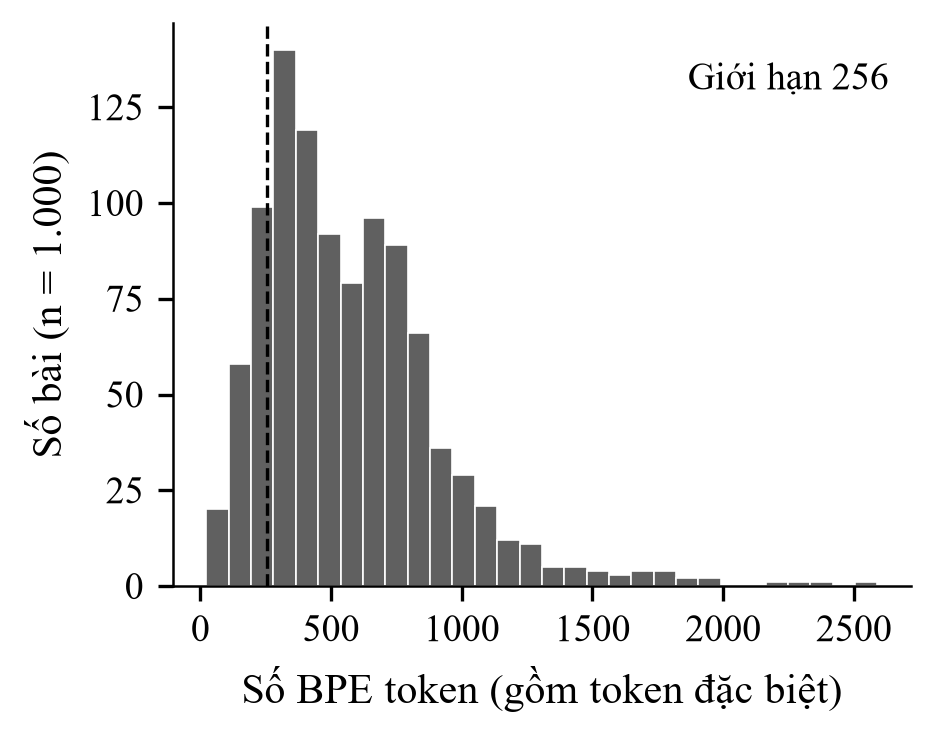
\includegraphics[width=\linewidth]{assets/compact/bpe_length.png}\caption{Độ dài BPE, gồm token đặc biệt.}\end{subfigure}\hfill
\begin{subfigure}[t]{.48\textwidth}\centering
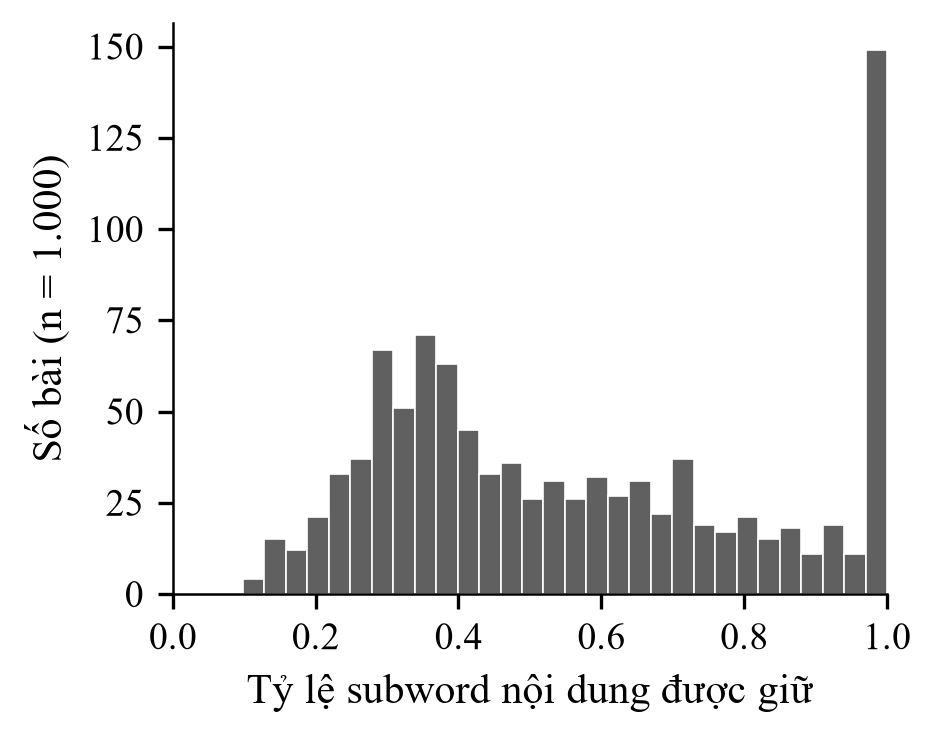
\includegraphics[width=\linewidth]{assets/compact/bpe_retention.png}\caption{Tỷ lệ subword nội dung được giữ.}\end{subfigure}
\caption{Khảo sát 1,000 bài: giới hạn 256 vị trí làm mất một phần đáng kể chuỗi đầu vào.}\label{fig:bpe-length-retention}\end{figure}
BiLSTM giới hạn 512 từ PyVi; trên tập dữ liệu cuối, 44.14\% bài vượt độ dài này và tỷ lệ từ giữ trung bình là 87.13\%. Hai kết quả không trực tiếp so với 56.32\% của PhoBERT: khác đơn vị, phạm vi khảo sát và tokenizer. SVM/LR dùng toàn văn nhưng nén văn bản thành vector thưa, làm mất thứ tự xa. Mỗi hướng giữ và bỏ loại thông tin khác nhau.


Một tỷ lệ giữ cao ở mức token chưa chứng minh những đoạn quyết định nhãn đã được giữ. Chẳng hạn, thông tin chủ đề có thể lặp ở mở đầu, hoặc chỉ rõ ở phần giữa bị cắt; thống kê chiều dài không phân biệt hai trường hợp. Ngược lại, bỏ một phần lớn token không nhất thiết làm mất tương ứng từng đó tín hiệu nếu bài chứa lặp và đoạn phụ. Báo cáo dùng thống kê để xác định mức độ phổ biến của cắt ngắn đầu vào, không đổi nó thành một ước lượng mất ngữ nghĩa.

\FloatBarrier


Nội dung dài nhất trong mảng tập dữ liệu có 131,081 ký tự, còn chuỗi chuẩn hóa dài nhất có 20,547 từ PyVi. Các cực trị cho thấy không thể giả định mọi bài nằm gần giá trị trung bình hoặc trung vị. Chúng cần được rà soát theo bài để phân biệt nội dung dài thật, đoạn liên quan và lỗi trích xuất. Báo cáo không dùng cực trị để suy một giới hạn cắt mới chưa được thử trên validation.

Giới hạn chuỗi tác động vào vị trí, còn từ vựng tác động vào kiểu token. BiLSTM có thể giữ đủ độ dài một bài nhưng vẫn thay từ lạ bằng UNK; PhoBERT có thể biểu diễn từ lạ bằng nhiều subword nhưng vì thế sớm đạt giới hạn 256 hơn. TF--IDF dùng toàn bài, song từ không thuộc từ vựng train hoặc bị bộ lọc số tài liệu chứa từ loại sẽ không có chiều riêng. Mỗi cơ chế mất thông tin khác nhau, nên ``không cắt bài'' không đồng nghĩa giữ toàn bộ thông tin văn bản.

Khảo sát BPE dùng mẫu cố định 1,000 bài giúp tái kiểm tra biểu đồ phân bố và tỷ lệ giữ mà không mã hóa lại tập dữ liệu. Kết quả phải đi cùng cỡ mẫu và seed, trong khi phân bố lớp/split dùng toàn tập dữ liệu cuối. Một biểu đồ mẫu có thể mô tả độ dài phổ biến nhưng chưa đại diện từng lớp ít bài với độ chính xác như toàn bộ mẫu. Khi đánh giá tác động cắt ngắn đầu vào theo nhãn, cần một phân tích có số mẫu và độ bất định riêng.


\section{Loại bỏ bài trùng lặp, phòng ngừa rò rỉ dữ liệu và giới hạn dữ liệu}
Nếu nhiều bản ghi có văn bản giống nhau sau chuẩn hóa nhưng nhãn khác nhau, cả nhóm bị loại thay vì tùy chọn một nhãn. Dòng lặp cùng nhãn được giữ một đại diện. Quy tắc này áp dụng trước khi chia tập, bỏ từ dừng và tăng trọng số tiêu đề, để bốn quy trình phân loại dựa trên cùng tập bài chứ không có bốn tập dữ liệu khác nhau do cách tạo đặc trưng.

Chín phép đối chiếu giữa ba tập theo URL, văn bản thô và văn bản chuẩn hóa không phát hiện giao nhau chính xác. Từ vựng BiLSTM và từ vựng/IDF TF--IDF chỉ học từ tập huấn luyện; validation/test dùng các biến đổi cố định. Đối chiếu mã băm trùng khớp chưa đánh giá bài viết lại, gần trùng hoặc nhiều bài về cùng sự kiện. Phép chia ngẫu nhiên cùng nguồn vì vậy không mô phỏng đầy đủ dự đoán tin tương lai.

Bộ nhớ đệm (cache) lưu kết quả xử lý để có thể dùng lại mà không tính toán từ đầu. Cache có mã nhận diện dữ liệu gắn bản dữ liệu, mapping, split và biểu diễn; số dòng bằng nhau chưa đủ để tái sử dụng cache. Mỗi notebook mô hình có cache riêng, không tham gia quá trình thực thi của app. Bản dữ liệu có thể còn quảng bá, đoạn liên quan hoặc nhiễu trích xuất, chưa được kiểm toán ngữ nghĩa toàn bộ. Dữ liệu sạch được hiểu là đạt quy tắc xác minh và kiểm tra đã công bố; đường dẫn tái hiện được tập trung tại Phụ lục~\ref{app:evidence}.

\chapter{Biểu diễn và kiến trúc bốn phương pháp}
\label{chap:model}
Chương~\ref{chap:related} xác định ba hướng biểu diễn được lựa chọn. Chương này mô tả đúng các cấu hình thực thi: TF--IDF với SVM/LR, LSTM hai chiều với embedding học từ đầu và PhoBERT-base-v2 có tiền huấn luyện. Các khác biệt về stopword, tiêu đề và đơn vị cắt được công khai để diễn giải kết quả so sánh.
\section{TF--IDF và hai bộ phân loại tuyến tính}
\label{sec:linear_models}
SVM và Logistic Regression dùng cùng cách tạo đặc trưng từ corpus chuẩn hóa. Sau khi chốt corpus và phép chia, tiêu đề đã phân đoạn được lặp thêm hai lần trước chuỗi tiêu đề--nội dung, tạo ba lần xuất hiện của tiêu đề. Hai notebook dùng danh sách stopword riêng nhưng có cùng nội dung, gồm 1.959 mục sau chuẩn hóa; hash bắt đầu \texttt{8560838c}. Stopword được loại ở bước biểu diễn cho mô hình, không dùng để xác định nhóm trùng của corpus chung.

\subsection{Từ tần suất đến vector thưa}
Với thuật ngữ $j$ và tài liệu $d$, biểu diễn dùng TF logarit, IDF có làm trơn và chuẩn hóa $L_2$:
\begin{align}
\operatorname{tf}_{d,j}&=1+\log n_{d,j}\quad(n_{d,j}>0),\\
\operatorname{idf}_j&=\log\frac{1+N_{train}}{1+\operatorname{df}_j}+1,\\
v_d&=\frac{\operatorname{tf}_d\odot\operatorname{idf}}{\|\operatorname{tf}_d\odot\operatorname{idf}\|_2}.
\end{align}
Từ vựng và IDF chỉ fit trên 139.975 mẫu train. Validation và test đi qua transform với các tham số đã cố định. Cấu hình được chọn giữ unigram và bigram, tối đa 150.000 đặc trưng, \texttt{min\_df=3}, \texttt{max\_df=0.98}; số chiều thực tế là 150.000. Không có SVD trong pipeline này. Các vector được lưu và tính toán dưới dạng thưa, không tạo ma trận dense toàn corpus.

Việc lặp tiêu đề tăng tần suất tín hiệu đầu bài, nhưng hệ số ba không có nghĩa giá trị TF--IDF cuối tăng đúng ba lần: TF logarit và chuẩn hóa $L_2$ còn biến đổi tỷ lệ. Bigram được tạo trên chuỗi ghép, nên cũng có thể xuất hiện ở ranh giới các lần lặp tiêu đề. Toàn văn không bị cắt theo số vị trí như mô hình neural, song thứ tự xa và cấu trúc lập luận không được giữ trong một vector TF--IDF \citep{kowsari2019}.

\subsection{SVM tuyến tính và Logistic Regression}
\texttt{LinearSVC} dùng regularization $L_2$, squared hinge loss và cơ chế một-chống-phần-còn-lại cho 20 lớp. Trong bộ phân loại lớp $c$, nhãn nhị phân $y_{i,c}\in\{-1,+1\}$ tạo hạng mất mát
\begin{equation}
\ell_{i,c}=\bigl[\max(0,1-y_{i,c}(w_c^\top v_i+b_c))\bigr]^2.
\end{equation}
Hệ số $C$ điều khiển đánh đổi regularization và mất mát. Điểm $s_c=w_c^\top v+b_c$ là margin, chưa phải xác suất; nhãn được chọn bằng argmax của 20 điểm. SVM trong thực nghiệm là tuyến tính, khác kernel RBF của một số nghiên cứu ở chương~\ref{chap:related}.

Logistic Regression dùng solver L-BFGS cho phân loại multinomial với regularization $L_2$. Logits tuyến tính được chuẩn hóa thành xác suất lớp:
\begin{equation}
p_c(v)=\frac{\exp(w_c^\top v+b_c)}{\sum_{j=1}^{20}\exp(w_j^\top v+b_j)}.
\end{equation}
Mục tiêu là log-loss có trọng số lớp, khác squared hinge của SVM. Cả hai có cùng thông tin từ vựng, nhưng nghiệm tối ưu và thang điểm khác nhau. Xác suất do LR học vẫn cần kiểm tra calibration; tối ưu log-loss không bảo đảm confidence đúng trên mọi nhóm bài.

\begin{table}[htbp]\centering\small\caption{Hai cấu hình tuyến tính được chọn bằng validation.}\label{tab:linear_config}
\begin{tabular}{lcc}\toprule Thuộc tính & SVM & Logistic Regression\\\midrule
Đặc trưng & \multicolumn{2}{c}{TF--IDF unigram/bigram, 150.000 chiều}\\
Trọng số lớp & balanced & balanced\\
$C$ & 0,5 & 3,0\\
Solver & liblinear, dual auto & L-BFGS\\
Ngưỡng hội tụ & $10^{-4}$ & $10^{-4}$\\
Số vòng tối ưu & 119 & 138\\
Giới hạn vòng & 5.000 & 500\\
Luồng CPU & 4 & 4\\\bottomrule
\end{tabular}\end{table}

\subsection{Đặc trưng học được và giới hạn diễn giải}
Hệ số dương lớn cho biết đặc trưng tăng điểm của lớp trong mô hình đã fit. Với Nông thôn mới, SVM có hệ số 3,1823 cho \texttt{nông\_thôn}; LR có hệ số 13,5690 cho cùng đặc trưng và 6,1810 cho bigram \texttt{xây\_dựng nông\_thôn}. Không so độ lớn giữa hai model như một thang quan trọng chung: mục tiêu, $C$ và thang score khác nhau. Hệ số cũng không phải tác động nhân quả hoặc một lời giải thích đầy đủ cho từng bài.

\begin{figure}[tbp]\centering
\begin{subfigure}[t]{.85\textwidth}\centering
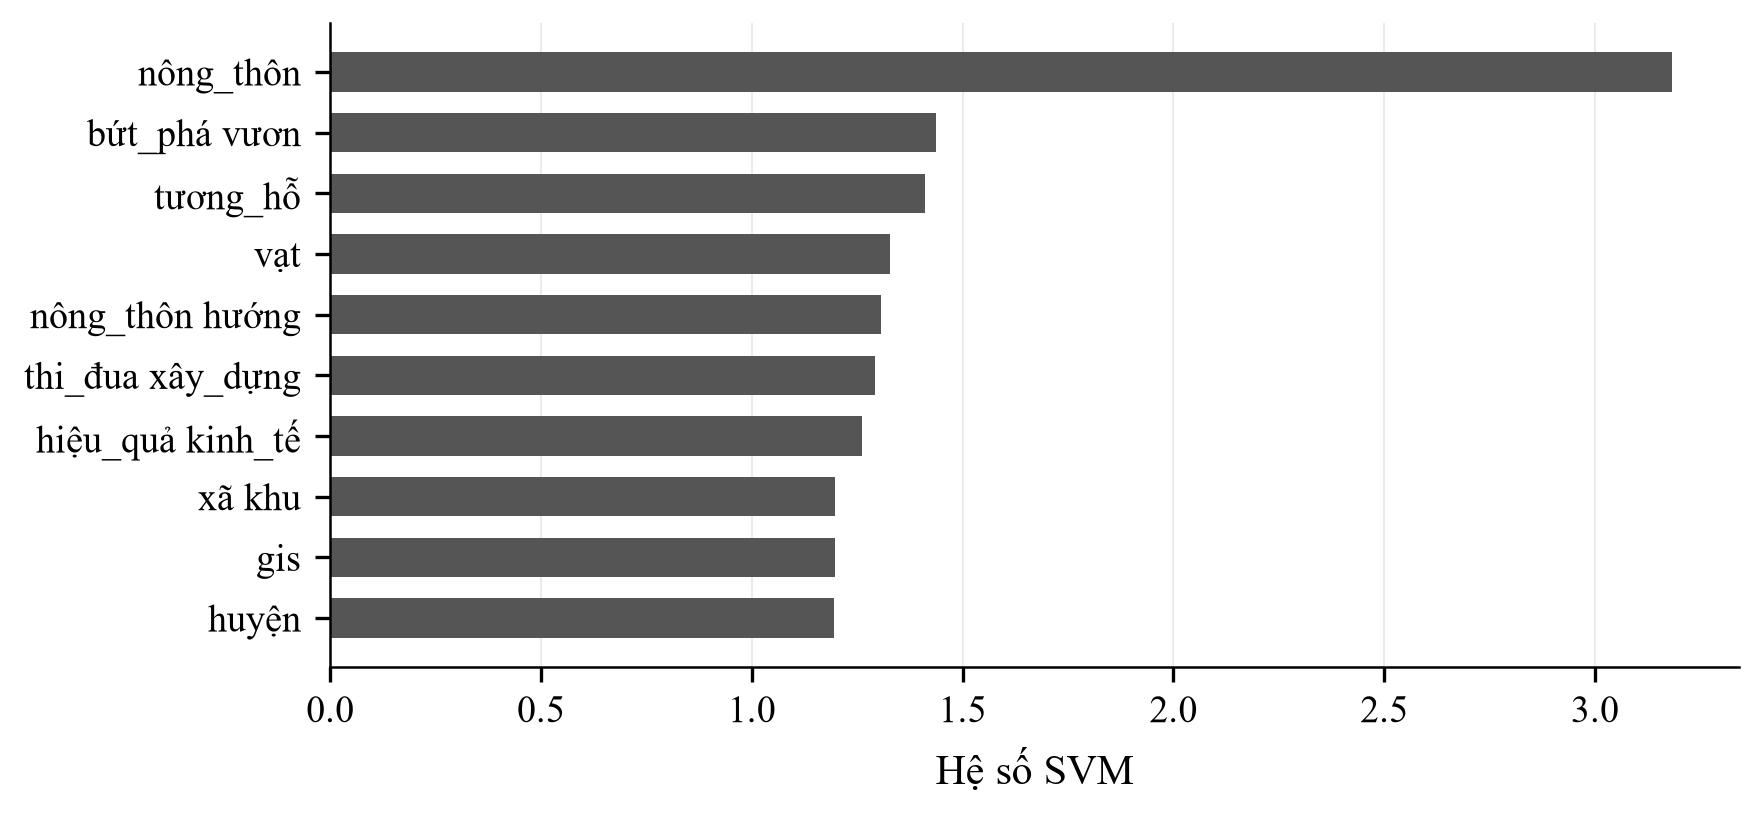
\includegraphics[width=\linewidth]{assets/compact/svm_features.png}\caption{Linear SVM.}\end{subfigure}\par\medskip
\begin{subfigure}[t]{.85\textwidth}\centering
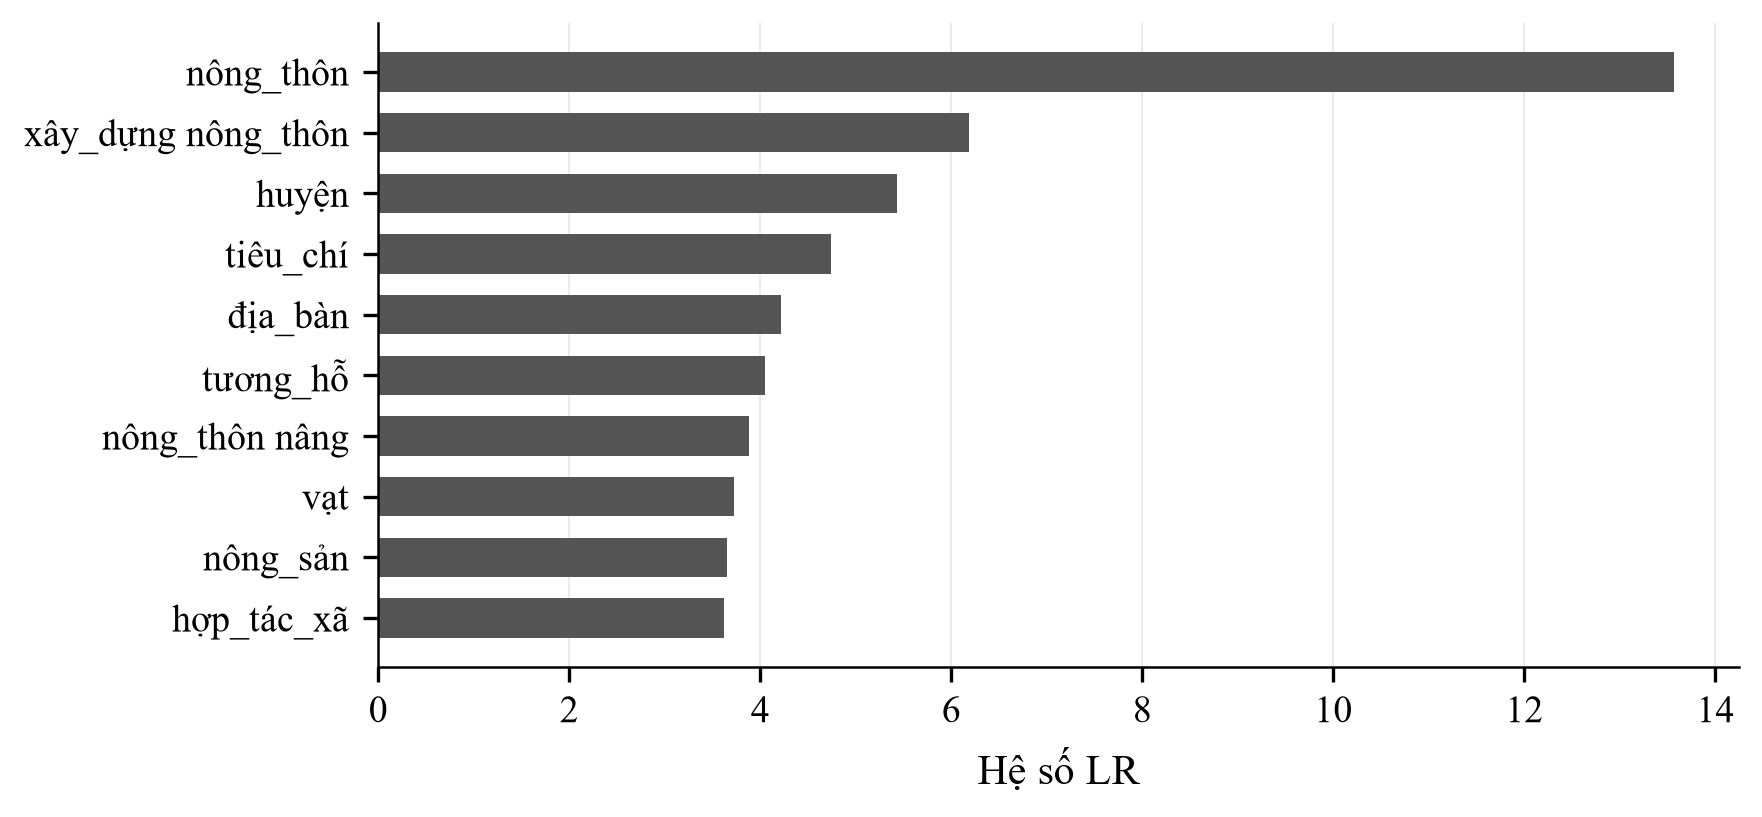
\includegraphics[width=\linewidth]{assets/compact/lr_features.png}\caption{Logistic Regression.}\end{subfigure}
\caption{Đặc trưng có hệ số dương lớn ở Nông thôn mới; thang hệ số không trực tiếp tương đương giữa hai model.}\label{fig:linear-features}\end{figure}

Việc bỏ stopword giảm một phần vốn từ thường xuất hiện, nhưng cũng có thể bỏ tín hiệu diễn ngôn hoặc cách viết của tòa soạn. N-gram còn khai thác cụm cục bộ sau bước lọc, với từ nhiều âm tiết đã được nối bằng PyVi. Vì thế, một bigram là hai đơn vị phân đoạn, không nhất thiết hai âm tiết cách trắng ban đầu. Vocabulary train cố định cũng có thể bỏ thuật ngữ mới ở test; khác biệt này không đồng nhất với UNK của model chuỗi.

Một hệ số lớn không có nghĩa mọi bài chứa term đó phải nhận nhãn tương ứng. Điểm tuyến tính còn cộng các đặc trưng khác và bias, trong khi giá trị term đã qua IDF cùng chuẩn hóa vector. Bỏ một term khỏi một bài có thể thay chuẩn hóa và làm đổi cả vector. Phân tích hệ số cung cấp tín hiệu toàn cục của model được fit, chưa là phép giải thích cục bộ có kiểm soát cho một dự đoán cụ thể.
\FloatBarrier

\section{Biểu diễn chuỗi và kiến trúc BiLSTM}
\label{sec:bilstm}
Phương pháp LSTM trong thiết kế được thực thi bằng biến thể hai chiều BiLSTM. Embedding được khởi tạo và học từ train, không nạp Word2Vec, PhoW2Vec hay encoder tiền huấn luyện. Chuỗi đầu vào giữ stopword và chỉ ghép tiêu đề một lần với nội dung. Vì vậy, đây là một đối chứng học biểu diễn tuần tự có giám sát, khác cả TF--IDF và PhoBERT có pretraining.

\subsection{Vocabulary, từ ngoài từ vựng và Head--Tail}
Vocabulary đếm từ trên train, lấy từ có tần suất ít nhất hai, sắp theo tần suất giảm rồi theo từ điển khi bằng nhau. Tổng 50.000 ID gồm PAD bằng 0, UNK bằng 1 và 49.998 từ. Token ngoài vocabulary được đưa về UNK; embedding PAD không được cập nhật như từ nội dung. Không học vocabulary từ validation/test để giảm tỷ lệ từ lạ một cách không hợp lệ.

Cấu hình được chọn giới hạn 512 \emph{từ đã phân đoạn}. Bài dài giữ 256 từ đầu và 256 từ cuối, không thêm BOS/EOS. Bài ngắn được giữ đầy đủ; mỗi batch pad đến độ dài lớn nhất của các mẫu trong batch, rồi dùng packed sequence để bỏ padding khỏi quá trình recurrent. Head--Tail vẫn bỏ phần giữa và nối hai đoạn không kề nhau, nhưng đơn vị cắt khác 254 subword nội dung của PhoBERT.

Trên corpus 199.965 bài, 44,14\% vượt 512 từ; tỷ lệ từ giữ trung bình là 87,13\%. Hai giá trị được tính từ độ dài đã xuất, không phải một lần tokenize mới. Tỷ lệ OOV trên toàn chuỗi train/validation/test lần lượt là 0,7782\%, 0,8714\% và 0,8696\%. Audit OOV tính trước cắt Head--Tail; không đồng nhất với tỷ lệ UNK trong tensor cuối hoặc lượng thông tin ngữ nghĩa bị mất.


Việc đặt UNK chỉ xử lý khả năng tra ID, không bổ sung nghĩa riêng cho mỗi từ lạ. Những từ ngoài vocabulary khác nhau cùng đi vào một embedding UNK; chúng vẫn có thể được phân biệt một phần bởi các từ bao quanh, nhưng thông tin từ vựng gốc đã mất. Tỷ lệ OOV thấp trên snapshot chưa dự báo tỷ lệ ở tin tương lai chứa tên riêng và thuật ngữ mới.

Packed sequence giúp trạng thái kết thúc phản ánh độ dài thật của bài, tránh recurrent tiếp tục quét nhiều PAD tới độ dài batch. Hai hướng đều quét chuỗi sau Head--Tail; hướng ngược không khôi phục phần giữa đã bị bỏ. Khi nối hai đoạn xa nhau, mô hình vẫn coi chúng là một chuỗi kề nhau, một giả định chung của cách cắt này với PhoBERT.



\subsection{Cơ chế cổng và trạng thái chuỗi}
LSTM duy trì hidden state $h_t$ cùng cell state $c_t$. Forget gate quyết định phần trạng thái cũ giữ lại, input gate điều chỉnh phần thông tin mới ghi vào, output gate điều chỉnh thông tin đưa ra hidden. Dạng cập nhật chuẩn giải thích vai trò của các cổng trong recurrent layer được dùng:
\begin{equation}c_t=f_t\odot c_{t-1}+i_t\odot\widetilde c_t,\qquad h_t=o_t\odot\tanh(c_t).\end{equation}
Các vector gate có giá trị sigmoid và được học từ embedding hiện tại cùng hidden trước đó; candidate cell dùng biến đổi phi tuyến. Đây là trạng thái theo chuỗi, không phải một đặc trưng TF--IDF được coi tùy ý như trục thời gian. Cổng cho phép điều chỉnh truyền thông tin nhưng không bảo đảm nhớ đủ mọi chi tiết qua một bài dài \citep{kowsari2019}.

Hai hướng của BiLSTM có tham số riêng và quét theo hai thứ tự ngược nhau. Chúng cung cấp hai cách tổng hợp cùng chuỗi đã giữ, rồi head nhận vector nối; số lớp recurrent vẫn là một, không biến thành mạng nhiều tầng vì có hai hướng. Dropout bên ngoài recurrent có vai trò regularization, không bổ sung token hoặc tri thức ngôn ngữ tiền huấn luyện.


\subsection{Trạng thái hai chiều và đầu phân loại}
Embedding có chiều 200; một recurrent layer có hidden size 128 cho mỗi hướng. Các cổng forget, input và output lần lượt điều chỉnh thông tin cũ giữ lại, thông tin mới ghi vào cell state và phần trạng thái được xuất theo chuỗi \citep{kowsari2019}. Mô hình quét chuỗi đã cắt ở cả hai hướng, rồi ghép trạng thái kết thúc phép quét xuôi và ngược:
\begin{equation}
r=[\overrightarrow h_{\mathrm{end}};\overleftarrow h_{\mathrm{end}}]\in\mathbb R^{256},\qquad
z=W\operatorname{Dropout}(r)+b\in\mathbb R^{20}.
\end{equation}
Trạng thái kết thúc hướng ngược không phải hidden tại vị trí cuối theo thứ tự đọc xuôi. Code lấy hai hidden cuối của hai hướng từ packed sequence, không lấy trung bình các token. Dropout 0,35 đặt sau embedding và trước lớp tuyến tính; recurrent dropout giữa các layer bằng 0 vì chỉ có một layer.

\begin{figure}[tbp]\centering
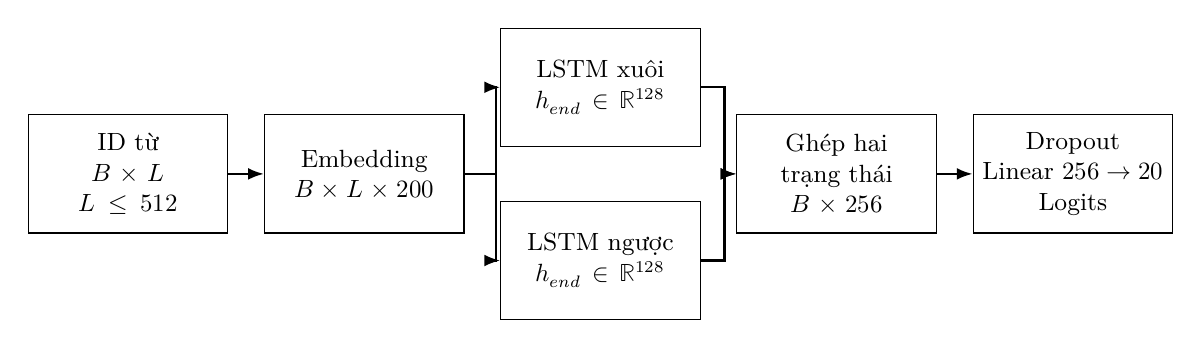
\begin{tikzpicture}[box/.append style={text width=23mm,minimum height=15mm}]
\node[box] (ids) at (0,0) {ID từ\\$B\times L$\\$L\le512$};
\node[box] (emb) at (3,0) {Embedding\\$B\times L\times200$};
\node[box] (fw) at (6,1.1) {LSTM xuôi\\$h_{end}\in\mathbb R^{128}$};
\node[box] (bw) at (6,-1.1) {LSTM ngược\\$h_{end}\in\mathbb R^{128}$};
\node[box] (cat) at (9,0) {Ghép hai\\trạng thái\\$B\times256$};
\node[box] (head) at (12,0) {Dropout\\Linear $256\to20$\\Logits};
\draw[flow] (ids)--(emb);
\draw[flow] (emb.east)--++(0.4,0)|-(fw.west);
\draw[flow] (emb.east)--++(0.4,0)|-(bw.west);
\draw[flow] (fw.east)--++(0.3,0)|-(cat.west);
\draw[flow] (bw.east)--++(0.3,0)|-(cat.west);
\draw[flow] (cat)--(head);
\end{tikzpicture}
\caption{BiLSTM thực thi trong notebook: embedding học từ đầu, packed sequence, ghép hidden cuối hai hướng và đầu phân loại 20 lớp. Dropout embedding được lược trong khối để giữ sơ đồ gọn.}
\label{fig:bilstm_arch}
\end{figure}

Model có 10.343.060 tham số: embedding chiếm 10.000.000, BiLSTM 337.920 và classifier 5.140. Phần lớn tham số thuộc bảng từ, không phải recurrent layer. Kích thước nhỏ hơn PhoBERT không tự xác định chất lượng; vocabulary, số từ giữ, cách tổng hợp chuỗi và chế độ pretraining đều khác nhau. Phần tiếp theo trình bày encoder ngữ cảnh và cấu hình PhoBERT được dùng trong cùng bài toán.

\FloatBarrier
\section{PhoBERT, BPE và Head--Tail}
Với tin tức giao thoa chủ đề, cùng một từ như ``thị trường'' có thể chỉ thị trường tài chính, du lịch hoặc tiêu dùng; encoder tạo biểu diễn phụ thuộc đoạn văn bản được giữ để cung cấp tín hiệu cho đầu phân loại.

Encoder Transformer tạo biểu diễn của mỗi vị trí dựa trên các vị trí còn lại trong đoạn văn bản được giữ. Mô hình tiền huấn luyện cung cấp tham số đã học các quy luật ngôn ngữ; fine-tuning điều chỉnh biểu diễn và đầu phân loại theo 20 nhãn của bài toán. BERT là một cơ sở của hướng học biểu diễn hai chiều và fine-tuning cho tác vụ downstream \citep{bert}; RoBERTa nghiên cứu các thay đổi trong quy trình tiền huấn luyện BERT \citep{roberta}. PhoBERT tập trung vào tiếng Việt \citep{phobert}.

Bài tập lớn sử dụng \texttt{vinai/phobert-base-v2}. Theo model card chính thức, bản base-v2 có quy mô khoảng 135 triệu tham số, độ dài tối đa 256 và corpus tiền huấn luyện gồm 20 GB Wikipedia/tin tức cùng 120 GB OSCAR-2301 \citep{phobertcard}. Corpus này là dữ liệu tiền huấn luyện của mô hình nền. Dataset dự án có 200.337 bài sạch theo chuyên mục; sau khử trùng văn bản, 199.965 bài được chia thành ba tập phục vụ fine-tuning và đánh giá. Báo cáo không coi số liệu hiệu năng của nhà phát triển PhoBERT ở các benchmark khác là kết quả của bài tập lớn.

\subsection{Phân đoạn từ và mã hóa BPE}
Sau PyVi, chuỗi được mã hóa bởi \texttt{PhobertTokenizer} cùng \texttt{vocab.txt} và \texttt{bpe.codes}. Các từ phổ biến có thể được biểu diễn gọn, trong khi một từ ít gặp có thể bị chia thành nhiều subword. Do đó, số token không bằng số từ, và một bài có cùng số từ với bài khác vẫn có thể cần số vị trí khác nhau.

Mã hóa sinh các ID số nguyên, không truyền chuỗi tiếng Việt trực tiếp vào mạng neural. ID được tra trong ma trận embedding; attention mask cho biết vị trí nào thuộc văn bản thật. Từ vựng có 64.001 mục, bao gồm các token đặc biệt. Trong cấu hình, token bắt đầu có ID 0, padding có ID 1 và token kết thúc có ID 2. Những ID này phải được lấy từ tokenizer tương ứng với checkpoint; thay tokenizer bằng một phiên bản khác có thể làm tensor vẫn đúng kích thước nhưng sai ý nghĩa.

Tokenizer và cấu hình nhãn là một phần của gói mô hình, cùng với trọng số và tham số hiệu chỉnh. Dịch vụ sử dụng \texttt{local\_files\_only=True}, nên suy luận không phụ thuộc vào việc tải một tokenizer mới từ mạng trong lúc khởi động. Đây là điều kiện quan trọng để đối chiếu notebook với ứng dụng.

\subsection{Lựa chọn Head--Tail cho bài báo dài}
Giới hạn 256 vị trí gồm cả hai token đặc biệt. Nếu chuỗi BPE không có token đặc biệt dài $L>254$, đầu vào được tạo như sau:
\begin{equation}
s=[\langle s\rangle,u_1,\ldots,u_{127},u_{L-126},\ldots,u_L,\langle/ s\rangle].
\end{equation}
Nếu $L\le254$, chuỗi được mã hóa đầy đủ, thêm token bắt đầu/kết thúc và padding đến 256 vị trí. Attention mask bằng 1 ở các vị trí có nội dung hoặc token đặc biệt và bằng 0 ở padding. Hai nhánh được kiểm tra ở các ranh giới 253, 254, 255 và 256 token để tránh lỗi thêm token đặc biệt hoặc cắt lệch một vị trí.

\HeadTailDiagram
Với bài dài, phần head có tiêu đề và đoạn mở đầu, trong khi phần tail có các đoạn kết. Giả thiết sử dụng là hai vùng này có thể chứa tín hiệu chủ đề hữu ích. Tuy nhiên, phần giữa có thể chứa lập luận, tên tổ chức hoặc sự kiện quyết định nhãn; toàn bộ vùng đó bị loại nếu vượt giới hạn. Head--Tail cũng nối hai vùng không kề nhau trong bản gốc thành hai đoạn kề nhau trong tensor. Không có dấu phân cách chuyên biệt để mô hình biết khoảng giữa bị bỏ.

Ở mức token, lựa chọn được thực hiện sau BPE nên có thể cắt giữa các subword của một từ. Điều này khác với lấy 127 từ đầu và 127 từ cuối. Các vị trí được đánh lại theo chuỗi ghép 256 token; chúng không giữ tọa độ tuyệt đối trong bài báo dài. Đây là một phép nén đầu vào có mất thông tin, không phải cơ chế attention trên toàn bộ bài.

\subsection{Chi phí và các phương án so sánh}
Attention chuẩn xét các cặp vị trí nên ma trận attention mỗi head có $L^2$ phần tử. Giới hạn $L=256$ giúp kiểm soát bộ nhớ và thời gian khi fine-tuning. Tăng gấp đôi chiều dài làm số phần tử ma trận cặp tăng gấp bốn, trước khi tính các chi phí khác. FFN và phép chiếu cũng đóng góp đáng kể; không thể mô tả toàn bộ runtime chỉ bằng hạng $L^2$.

Các phương án cần so sánh trong một thực nghiệm bổ sung gồm head-only, tail-only, lấy đoạn trượt với tổng hợp logits, biểu diễn phân cấp theo đoạn và encoder ngữ cảnh dài. Sản phẩm hiện có một cấu hình Head--Tail; không có phép ablation đã huấn luyện để chứng minh cấu hình này tối ưu hoặc tốt hơn head-only bao nhiêu. Số liệu độ dài hỗ trợ lý do nghiên cứu cách cắt, nhưng không thay thế phép so sánh thực nghiệm.

\subsection{Cấu hình kiến trúc thực tế}
\begin{table}[htbp]\centering\caption{Thông số đọc từ config.json của checkpoint.}\small
\begin{tabular}{lr}\toprule
Thuộc tính & Giá trị\\\midrule
Kiến trúc & RobertaForSequenceClassification\\
Số lớp encoder & 12\\
Hidden size & 768\\
Attention heads & 12\\
Chiều mỗi head & 64\\
Intermediate size & 3.072\\
Vocabulary size & 64.001\\
Max position embeddings & 258\\
Activation & GELU\\
Số nhãn đầu ra & 20\\\bottomrule
\end{tabular}\end{table}
Giá trị 258 của bảng vị trí không có nghĩa hệ thống nhận bài dài 258 token văn bản. Giới hạn pipeline là 256, còn chỉ số vị trí của RoBERTa có quy ước liên quan đến padding và offset. Không sử dụng một decoder sinh token hay cross-attention; cấu hình \texttt{is\_decoder=False} và \texttt{add\_cross\_attention=False} phù hợp với encoder phân loại.

\EncoderDiagram
Với batch $B$, input IDs và mask có kích thước $B\times256$. Embedding và mỗi tầng encoder tạo tensor $B\times256\times768$. Đầu phân loại lấy biểu diễn vị trí đầu tiên và sinh logits $B\times20$. Vị trí đầu là token tổng hợp cho tác vụ phân loại; đây không phải lấy trung bình các token và cũng không phải sử dụng một vector TF--IDF.

\FloatBarrier
\section{Cơ chế self-attention, encoder và đầu phân loại}\subsection{Embedding và thông tin vị trí}
Embedding đầu vào kết hợp vector token, vị trí và token type. Bộ token type có một loại trong cấu hình này, nên không tạo hai segment độc lập cho tiêu đề và nội dung. LayerNorm và dropout được áp dụng trong thành phần embedding trước encoder. Vector vị trí giúp mạng phân biệt thứ tự, vì phép attention tự nó không biết một từ đứng ở đầu hay cuối nếu không có thông tin vị trí.

Vì chuỗi Head--Tail được ghép trước khi mã hóa qua encoder, embedding vị trí thể hiện thứ tự của chuỗi đã ghép. Mạng có thể học đặc trưng của đoạn đầu và đoạn cuối trong cách biểu diễn này, nhưng không được cung cấp số token bị loại ở giữa. Một giả thuyết cải thiện là bổ sung cơ chế biểu diễn theo đoạn; giả thuyết đó cần thay đổi thiết kế và đánh giá riêng.

\subsection{Self-attention và xử lý theo ngữ cảnh}
Theo cơ chế attention của Transformer \citep{attention}, ở một head, biểu diễn $H$ được chiếu thành query, key và value:
\begin{equation}
Q=HW_Q,\quad K=HW_K,\quad V=HW_V.
\end{equation}
Các độ tương thích được chuẩn hóa theo chiều head và chuyển thành trọng số:
\begin{equation}
A=\operatorname{softmax}\left(\frac{QK^\top}{\sqrt{d_k}}+M\right),\qquad O=AV,\quad d_k=64.
\end{equation}
$M$ là attention mask đã chuyển thành dạng cộng để các vị trí padding không được chọn làm key hữu ích. Attention trong encoder là hai chiều trên các vị trí hợp lệ, không dùng causal mask kiểu dự đoán token tiếp theo. Nhờ vậy, một vị trí có thể kết hợp ngữ cảnh ở cả phía trước và phía sau trong đoạn được giữ.

\AttentionDiagram
Mười hai head cung cấp các phép chiếu học được khác nhau; đầu ra được nối và chiếu về chiều 768. Không nên gán sẵn mỗi head cho một chức năng như ``nhận biết pháp luật'' nếu chưa có phân tích thực nghiệm. Attention là thành phần tính toán tạo biểu diễn, không tự động là lời giải thích nhân quả của nhãn cuối.

\subsection{Residual, LayerNorm và feed-forward}
Mỗi tầng có residual connection và LayerNorm quanh các thành phần attention và FFN theo kiến trúc RoBERTa. Residual tạo đường truyền để biểu diễn đầu vào được giữ cùng phần biến đổi học được. LayerNorm ổn định thang giá trị trong chiều đặc trưng. FFN áp dụng các phép chiếu tại từng vị trí với chiều trung gian 3.072 và activation GELU, rồi trả về 768.

Attention cho phép trao đổi thông tin giữa các vị trí; FFN biến đổi đặc trưng của từng vị trí sau trao đổi. Qua 12 tầng, biểu diễn đầu vào không còn là vector từ độc lập mà đã kết hợp các quan hệ trong đoạn văn bản. Tuy nhiên, mọi quan hệ vẫn giới hạn ở các token đã chọn. Không tầng nào có thể đọc lại đoạn giữa bị bỏ bởi Head--Tail.

\subsection{Đầu phân loại và logits}
\texttt{RobertaForSequenceClassification} sử dụng đầu phân loại trên hidden state của token đầu, gồm dropout, dense $768\to768$, tanh, dropout và phép chiếu $768\to20$. Dropout hoạt động ở chế độ train; dịch vụ gọi \texttt{eval()} để tắt ngẫu nhiên dropout khi suy luận. Logits là điểm chưa chuẩn hóa; chúng có thể âm hoặc dương và không phải xác suất.

Softmax chuẩn chuyển logits thành phân bố:
\begin{equation}
p_c=\frac{\exp(z_c)}{\sum_{j=1}^{20}\exp(z_j)}.
\end{equation}
Xác suất tổng bằng 1 giữa 20 lớp trong taxonomy. Điều đó không bảo đảm bài nằm trong taxonomy hoặc xác suất là ước lượng đúng của xác suất thực. Một đầu vào ngoài miền vẫn bị buộc vào một trong 20 lớp nếu không có cơ chế từ chối độc lập.

\subsection{Quy mô tham số và ý nghĩa của fine-tuning}
Checkpoint có 135.013.652 tham số. Embedding chiếm 49.353.216; 12 lớp encoder chiếm 85.054.464; đầu phân loại chiếm 605.972. Tổng số tham số được tính từ kiến trúc và tensor của gói mô hình, không suy ra bằng cách làm tròn nhãn ``135M''.

Fine-tuning cập nhật mô hình cho tác vụ chuyên mục, thay vì tiền huấn luyện lại từ đầu trên corpus tin tức này. Đầu phân loại tương thích 20 lớp được khởi tạo khi tạo mô hình cho tác vụ; encoder nhận tham số mô hình nền. Toàn bộ quá trình dùng nhãn giám sát của corpus. Đối chứng ở chương~\ref{chap:comparison} cho biết hiệu quả các pipeline trên cùng test, nhưng chưa cô lập phần lợi ích riêng của pretraining khỏi kiến trúc và biểu diễn.



Ở bước fine-tuning, gradient của head truyền qua biểu diễn $h_0$ vào encoder và embedding. Encoder được cập nhật nhưng vẫn khởi đầu từ tri thức của checkpoint nền; ``train từ đầu'' trong một lượt fresh không có nghĩa khởi tạo ngẫu nhiên toàn PhoBERT. Điều đó khác BiLSTM, nơi cả bảng embedding lẫn recurrent layer học từ corpus có giám sát. Đối chứng không có một PhoBERT khởi tạo ngẫu nhiên cùng kiến trúc để định lượng riêng đóng góp tiền huấn luyện.

\subsection{Đọc một head attention và giới hạn giải thích}
Với một bài, $Q,K,V$ của từng head có 256 hàng và 64 chiều; ma trận $QK^\top$ có $256\times256$ điểm. Softmax theo các vị trí key cho mỗi query tạo trọng số để tổng hợp các hàng của $V$. Hệ số $1/\sqrt{d_k}$ điều chỉnh thang dot product trước chuẩn hóa; nó không là hệ số quyết định theo lớp $\tau_c$. Padding mask tác động đến các vị trí được dùng làm key, không mang nhãn chuyên mục.

Mười hai head học các phép chiếu khác nhau, rồi nối đầu ra trước chiếu về chiều 768. Residual giữ đường truyền biểu diễn ban đầu cạnh phần biến đổi; FFN chuyển đặc trưng tại từng vị trí sau trao đổi thông tin. Qua nhiều tầng, token đầu có thể tổng hợp tín hiệu của đoạn đã giữ. Tuy nhiên, attention weight lớn không tự chứng minh token gây ra nhãn; muốn giải thích nhân quả cần một thiết kế perturbation hoặc attribution riêng, chưa có trong project.

\FloatBarrier
\section{Đối chiếu thông tin đầu vào và giới hạn diễn giải}
Bốn pipeline cùng giải một bài toán và được đánh giá trên cùng tập test, nhưng không sử dụng cùng cơ chế biểu diễn hoặc lượng văn bản quan sát. SVM/LR khai thác TF--IDF toàn văn với tiêu đề tăng tần suất; BiLSTM xử lý tối đa 512 từ; PhoBERT sử dụng 256 subword với tiền huấn luyện. Vì vậy, chênh lệch thực nghiệm phản ánh toàn bộ cấu hình xử lý, chưa cô lập đóng góp riêng của kiến trúc.

BiLSTM có thể học trật tự token trong chuỗi nhưng chưa có tri thức từ một corpus tiền huấn luyện. PhoBERT có tri thức ngôn ngữ nền song chỉ nhìn đoạn đã giữ; TF--IDF quan sát phần giữa mà hai model neural có thể bỏ. Một đối chứng cố định lượng thông tin, nguồn embedding và ngân sách tối ưu cần được thiết kế riêng trước khi kết luận nguyên nhân của khoảng cách F1.

\chapter{Huấn luyện, lựa chọn cấu hình và hiệu chỉnh}\label{chap:training}
\FloatBarrier
\section{Giao thức lựa chọn và thông số thực nghiệm}
Các mô hình dùng cùng tập dữ liệu và phép chia, nhưng có mục tiêu tối ưu, trọng số và ngân sách lựa chọn khác nhau. Tất cả cấu hình được đánh giá trên test được chọn bằng validation. Từ vựng/IDF, từ vựng chuỗi và trọng số lớp chỉ học từ train; test không dùng chọn cấu hình, epoch, temperature hoặc hệ số quyết định.
\begin{table}[htbp]\centering\small\caption{Thiết lập lựa chọn và thiết bị; cấu hình biểu diễn chi tiết ở chương~\ref{chap:model}.}\label{tab:training_protocol}
\begin{tabularx}{\linewidth}{lXXl}\toprule Mô hình & Ngân sách lựa chọn & Tiêu chí và tối ưu & Thiết bị\\\midrule
SVM & 12 cấu hình; chỉ học từ tập huấn luyện TF--IDF & Hội tụ squared hinge; Macro-F1 validation & CPU, 4 luồng\\
LR & 12 cấu hình; chỉ học từ tập huấn luyện TF--IDF & Hội tụ mất mát logarit; Macro-F1 validation & CPU, 4 luồng\\
BiLSTM & 3 cấu hình; tối đa 10 epoch/lượt & AdamW; bản lưu mô hình theo Macro-F1 & RTX A3000\\
PhoBERT & Cấu hình cố định; tối đa 7 epoch & AdamW; bản lưu mô hình theo Macro-F1 & RTX A3000\\\bottomrule
\end{tabularx}\end{table}
Validation còn được dùng ước lượng tham số hiệu chỉnh nên kết quả có phụ thuộc vào tập này; một tập hiệu chỉnh xác suất riêng là hướng kiểm tra thêm. Seed 42 khóa phép chia trong bản dữ liệu, chưa bảo đảm phép tính GPU giống bit giữa thiết bị/phiên bản. Ngân sách tìm cấu hình khác nhau cần được giữ khi diễn giải đánh đổi, thay vì coi đây là một phép thay kiến trúc có kiểm soát mọi yếu tố.

\FloatBarrier
\section{Huấn luyện SVM/LR và BiLSTM}
\section{Huấn luyện và lựa chọn hai mô hình tuyến tính}
SVM và LR mỗi model khảo sát 12 cấu hình từ hai profile unigram/unigram--bigram, ba giá trị $C\in\{0,5;1,5;3,0\}$ và hai chính sách trọng số lớp uniform/balanced. Các profile được fit độc lập chỉ trên train; classifier dùng cùng ma trận của profile tương ứng. Với balanced, trọng số $w_c=N_{train}/(20n_c)$ dựa trên phân bố train, không cân bằng lại validation/test.

Validation chọn cấu hình bằng Macro-F1, tiếp đến Weighted-F1 và Accuracy khi bằng nhau. Mỗi cấu hình phải đạt hội tụ trước khi đủ điều kiện được chọn. Output xác nhận cả 12 cấu hình SVM và 12 cấu hình LR hội tụ; cấu hình được giữ là hai cấu hình trong bảng~\ref{tab:linear_config}. Không lấy cấu hình tốt nhất theo test và không refit thêm validation vào train sau lựa chọn. Chi phí tìm cấu hình được ghi riêng với thời gian fit classifier đã chọn.

\section{Huấn luyện BiLSTM và chọn checkpoint}
\label{sec:lstm_training}
Ba cấu hình khảo sát kết hợp Head--Tail 256/512 từ với số mũ trọng số lớp 0,5/1,0; các thành phần kiến trúc còn lại giữ như mục~\ref{sec:bilstm}. Báo cáo phân tích cấu hình được chọn: 512 từ, embedding 200, hidden 128 mỗi hướng, một layer, dropout 0,35 và $\alpha=0,5$. Trọng số được chuẩn hóa theo trung bình có trọng số của train:
\begin{equation}
\widetilde w_c=\left(\frac{N_{train}}{20n_c}\right)^{\alpha},\qquad
w_c=\frac{\widetilde w_c}{\sum_j(n_j/N_{train})\widetilde w_j}.
\end{equation}
Nông thôn mới có trọng số 3,3510 trong cấu hình này, khác 10,3226 của PhoBERT. Loss của batch là tổng cross-entropy có trọng số chia tổng trọng số các nhãn trong batch. Loss epoch được cộng từ các tử số và mẫu số, không lấy trung bình không trọng số giữa batch đầy và batch cuối.

\begin{table}[H]\centering\small\caption{Tối ưu BiLSTM của cấu hình được chọn.}\label{tab:bilstm_training}
\begin{tabular}{lr}\toprule Thiết lập & Giá trị\\\midrule
Optimizer & AdamW\\
Learning rate ban đầu / tối thiểu & $10^{-3}$ / $10^{-5}$\\
Weight decay / gradient clip & $10^{-4}$ / 1,0\\
Batch train / validation và test & 64 / 128\\
Epoch tối đa / epoch đã chạy & 10 / 10\\
Checkpoint chọn & Epoch 10\\
Early stopping patience / min delta & 2 / 0,001\\
ReduceLROnPlateau factor / patience & 0,5 / 0\\
GPU / precision & RTX A3000 12 GB / BF16\\\bottomrule
\end{tabular}\end{table}

AdamW cập nhật embedding, recurrent layer và classifier. AMP dùng BF16; gradient được clip về norm tối đa 1,0 trước bước optimizer. Scheduler theo Macro-F1 validation, giảm learning rate một nửa sau epoch không cải thiện đủ ngưỡng tuyệt đối 0,001. Batch giữ phân bố train thực tế qua shuffle; trọng số loss không tương đương oversampling lớp hiếm.

Checkpoint và early stopping có tiêu chí khác nhau: checkpoint giữ giá trị validation tốt nhất kể cả cải thiện nhỏ; bộ đếm dừng cần vượt mốc tốt trước đó ít nhất 0,001. Vì vậy, epoch 10 có Macro-F1 0,8449 cao nhất nhưng vẫn kích hoạt bộ đếm patience sau hai epoch không cải thiện đủ ngưỡng. Thực nghiệm đã chạy 10 epoch; không mô tả như được dừng trước giới hạn. Bảng và các đồ thị dưới đây thuộc duy nhất cấu hình được chọn, không nối lịch sử của ba cấu hình.
\DataTable{tables/lstm_epochs.tex}{Lịch sử 10 epoch của BiLSTM được chọn; loss có trọng số, checkpoint theo Macro-F1.}
Loss validation thấp nhất ở epoch 5 (0,4230), trong khi Macro-F1 cao nhất ở epoch 10 (0,8449). Loss train giảm từ 1,2428 xuống 0,2360; loss validation cuối là 0,4341. Chênh lệch này cảnh báo về mức phù hợp giữa train và validation, nhưng không đủ để quy mọi thay đổi F1 cho overfitting. Weighted loss, Macro-F1 và calibration đánh giá các tính chất khác nhau.
\ReportFigure{assets/baselines/lstm/training/train_loss.png}{Weighted cross-entropy train của BiLSTM qua 10 epoch, xuất riêng từ notebook.}
\ReportFigure{assets/baselines/lstm/training/validation_loss.png}{Loss validation của BiLSTM; cực tiểu loss không trùng checkpoint Macro-F1 tốt nhất.}
\ReportFigure{assets/baselines/lstm/training/validation_f1_macro.png}{Macro-F1 validation của BiLSTM; checkpoint được chọn ở epoch 10.}
\ReportFigure{assets/baselines/lstm/training/learning_rate.png}{Learning rate theo epoch của BiLSTM; giảm từ 0,001 đến 0,000125.}

\section{Hiệu chỉnh điểm số của các mô hình đối chứng}
SVM tạo margin, LR và BiLSTM tạo logits. Cả ba dùng $p(T)=\operatorname{softmax}(s/T)$, tìm $T>0$ bằng NLL trên validation và cố định trước đánh giá test. SVM dùng phép chuẩn hóa margin thành phân bố, không có xác suất sinh sẵn từ \texttt{LinearSVC}. Temperature dương giữ thứ tự score, nên Accuracy, precision, recall và F1 không thay đổi. Ba đối chứng không dùng hệ số điều chỉnh quyết định theo lớp như PhoBERT.

Validation phục vụ cả lựa chọn model lẫn fit temperature. Việc dùng lại validation có thể tăng phụ thuộc vào tập này; test vẫn không tham gia fit. Khoảng tin cậy trong notebook dùng bootstrap IID 500 lần trên test với model cố định. Nó mô tả biến thiên do mẫu đánh giá, không mô phỏng nhiều lần huấn luyện với seed khác nhau. So sánh ghép cặp ở chương~\ref{chap:comparison} giữ chung các mẫu bootstrap để đánh giá chênh lệch giữa model.

\section{Fine-tuning và hiệu chỉnh PhoBERT}
Các mục sau mô tả quy trình PhoBERT; trọng số, optimizer, lịch học và hệ số quyết định thuộc cấu hình riêng của mô hình. Phép chia và tiêu chí đánh giá thống nhất với ba đối chứng, còn cách biểu diễn và ngân sách tìm tham số khác nhau. Mọi kết luận về đóng góp riêng của Head--Tail, trọng số lớp hoặc pretraining cần một ablation tương ứng.




Điều kiện hội tụ của SVM/LR xác nhận optimizer đã đạt tiêu chí số của cấu hình, không chứng minh mô hình tối ưu về nhãn hay tổng quát hóa. Với LR, L-BFGS tối ưu mất mát logarit có điều chuẩn; với LinearSVC, mục tiêu squared hinge theo các bài toán một-chống-còn-lại. Cùng Macro-F1 validation để lựa chọn không làm hai mục tiêu train trở thành giống nhau. Số vòng tối ưu vì thế không so trực tiếp như số epoch của mạng nơ-ron.

Mỗi cấu hình ứng viên được học từ train trước khi đo trên validation. Không dùng test để loại cấu hình ứng viên hội tụ nhưng có điểm thấp, và không gộp train/validation rồi ước lượng lại một gói mô hình có điều kiện khác với gói mô hình đo test. Kết quả được báo cáo thuộc cấu hình đã chọn, còn chi phí tìm cấu hình tính toàn bộ ứng viên. Khoảng giữa thời gian huấn luyện cấu hình được chọn và tìm cấu hình phản ánh khác biệt giữa dùng lại một thiết lập và tìm ra thiết lập đó.

Với BiLSTM, loss train giảm chưa là tiêu chí nạp bản lưu mô hình cuối. Chọn bản lưu mô hình theo Macro-F1 và bộ đếm early stopping có ngưỡng cải thiện riêng, nên một epoch có thể tạo bản lưu mô hình tốt nhất dù không đặt lại bộ đếm dừng sớm. Cơ chế này giải thích vì sao lịch sử đủ 10 điểm và bản lưu được chọn ở epoch 10 cùng tồn tại; không cần suy một đợt train khác hoặc nối hai lịch sử.

\FloatBarrier
\section{Fine-tuning PhoBERT và diễn biến validation}
Mô hình khởi tạo từ \texttt{vinai/phobert-base-v2}; đầu phân loại 20 lớp được tạo cho tác vụ. Toàn bộ encoder và đầu phân loại được cập nhật qua lan truyền ngược, không giữ cố định bộ mã hóa nền. Train tensor có $139{,}975\times256$ vị trí; validation/test có $29{,}995\times256$. Input IDs, attention mask và nhãn giữ thứ tự, train shuffle batch còn các tập đánh giá giữ phân bố thực tế.

Với $n_c$ là số bài lớp $c$ trong train, PhoBERT dùng balanced weight:
\begin{equation}w_c=\frac{N_{train}}{20n_c},\qquad
\mathcal L_{\mathcal B}=\frac{-\sum_{i\in\mathcal B}w_{y_i}\log p_{i,y_i}}{\sum_{i\in\mathcal B}w_{y_i}}.\end{equation}
Không tăng thêm trọng số cho một chuyên mục bằng hệ số đặt thủ công. Nông thôn mới, Dân tộc thiểu số và miền núi, Kinh doanh có trọng số lần lượt 10.3226; 9.1847; 0.7908. Trọng số thay đổi mức đóng góp của lỗi, không bổ sung dữ liệu hoặc làm sạch nhãn; nếu lớp nhỏ có nhiễu, tăng mức phạt trong hàm mất mát có thể khuếch đại ảnh hưởng đó. Mất mát đánh giá có trọng số cũng khác NLL hiệu chỉnh xác suất không trọng số.

\begin{table}[htbp]\centering\small\caption{Cấu hình fine-tuning PhoBERT trên một RTX A3000 Laptop 12 GB.}
\begin{tabular}{lr}\toprule Thiết lập & Giá trị\\\midrule
Batch train / tích lũy gradient & 32 / 2\\
Effective batch / batch đánh giá & 64 / 64\\
Optimizer / weight decay & AdamW fused / 0.01\\
Learning rate cực đại / warmup & $2\times10^{-5}$ / 200 bước\\
Độ chính xác số / TF32 & BF16 / bật\\
Epoch tối đa / bản lưu được chọn & 7 / 7\\
Dừng sớm: số epoch chờ / mức cải thiện & 2 / 0.001\\
Evaluation và lưu bản lưu mô hình & Cuối mỗi epoch\\
Lưu lại tính toán gradient / biên dịch mô hình & Tắt / tắt\\\bottomrule
\end{tabular}\end{table}
AdamW tách weight decay khỏi cập nhật thích nghi \citep{adamw}. Scheduler warmup 200 bước rồi giảm theo tiến độ. Mỗi epoch có $\lceil139{,}975/32\rceil=4{,}375$ mini-batch, tạo 2,188 bước cập nhật sau tích lũy; bảy epoch có 15,316 bước. Batch cuối có thể nhỏ hơn effective batch 64, nên con số này là kích thước danh nghĩa.

Trainer chọn bằng Macro-F1 validation và nạp bản lưu mô hình tốt nhất ở cuối. Lần thực nghiệm chạy đủ bảy epoch; không mô tả như dừng sớm. Loss validation nhỏ nhất epoch 3 là 0.3548, trong khi bản lưu mô hình chọn epoch 7 có Macro-F1 khoảng 0.8723. Bảng~\ref{tab:pho_epochs} giữ mốc validation; test không dùng đổi tiêu chí sau khi xem kết quả.
\begin{table}[htbp]\centering\small\caption{Đánh giá cuối epoch trên validation PhoBERT.}\label{tab:pho_epochs}
\begin{tabular}{rrr}\toprule Epoch & Val loss & Val Macro-F1\\\midrule
1 & 0,4034 & 0,8343\\
2 & 0,3581 & 0,8538\\
3 & 0,3548 & 0,8597\\
4 & 0,3717 & 0,8660\\
5 & 0,4257 & 0,8718\\
6 & 0,4592 & 0,8708\\
7 & 0,4980 & 0,8723\\
\bottomrule\end{tabular}
\end{table}
\begin{figure}[tbp]\centering
\begin{subfigure}[t]{.48\textwidth}\centering
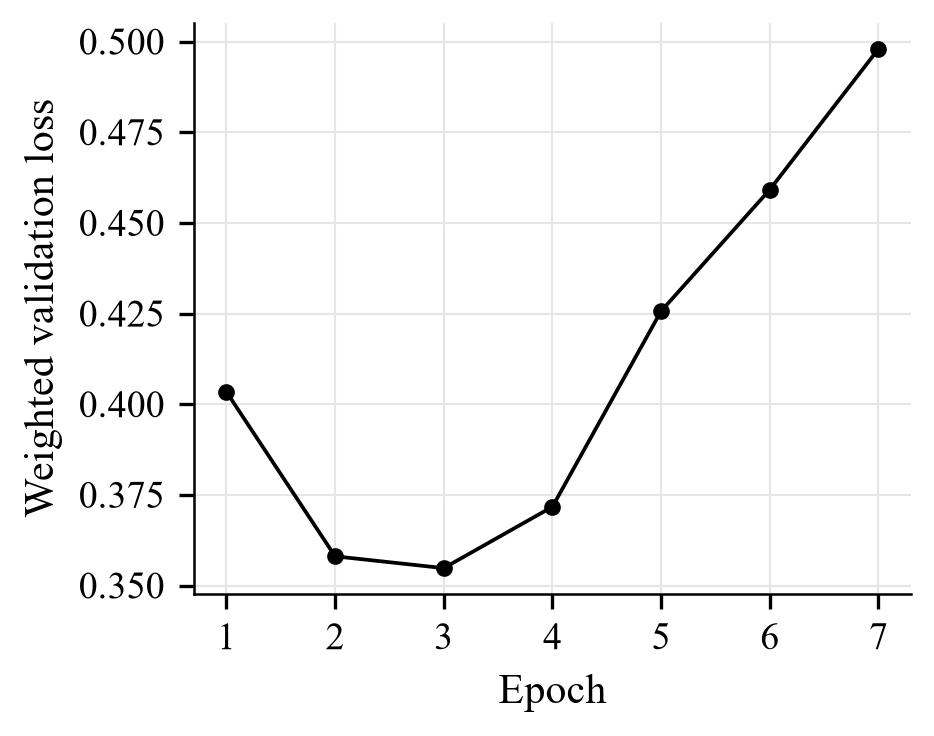
\includegraphics[width=\linewidth]{assets/compact/pho_val_loss.png}\caption{Mất mát trên tập xác thực có trọng số.}\end{subfigure}\hfill
\begin{subfigure}[t]{.48\textwidth}\centering
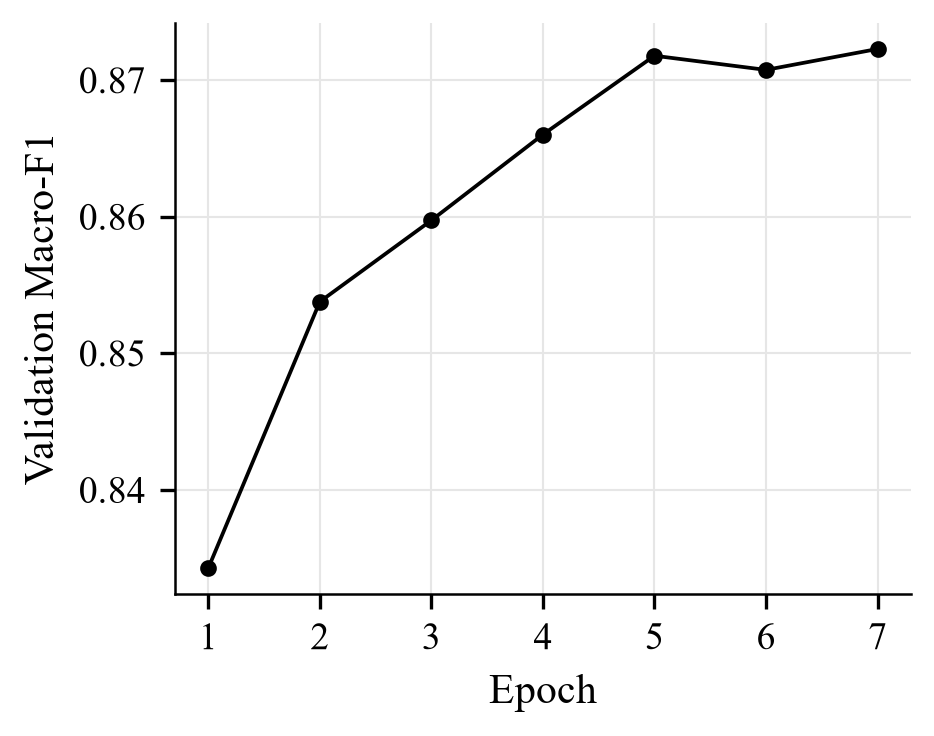
\includegraphics[width=\linewidth]{assets/compact/pho_val_f1.png}\caption{Macro-F1 trên tập xác thực.}\end{subfigure}
\caption{PhoBERT qua bảy epoch; lựa chọn bản lưu mô hình theo Macro-F1 không trùng cực tiểu loss.}\label{fig:phobert-validation}\end{figure}
Loss tăng về cuối trong khi F1 nhích lên phản ánh hai mục tiêu đánh giá khác nhau. Một số bài sai với xác suất tự tin có thể tăng mất mát logarit mà không làm đổi số nhãn đúng theo cùng cách. Đây là cách diễn giải cần đối chiếu với hiệu chỉnh xác suất; các đường học không tự chứng minh một cơ chế lỗi riêng hay xác lập epoch tối ưu cho mọi seed. Không so train loss ghi theo bước với validation loss như hai đại lượng được tổng hợp đồng nhất.



\subsection{Chọn bản lưu mô hình theo mục tiêu đánh giá}
Argmax và mất mát logarit phản ứng khác nhau với một thay đổi logits. Nếu xác suất nhãn tham chiếu thay đổi nhưng nhãn đứng đầu giữ nguyên, F1 không đổi; hàm mất mát có trọng số vẫn đổi. Nếu một số bài của lớp nhỏ đổi từ sai sang đúng, Macro-F1 có thể tăng đáng kể dù nhiều bài khó khác bị tự tin sai hơn. Bởi vậy, chọn bản lưu mô hình theo F1 và theo cực tiểu validation loss có thể dẫn tới hai trọng số khác nhau mà không có mâu thuẫn số liệu.

Bản lưu mô hình được xác định bằng validation sau từng epoch; test chỉ được dùng sau khi lựa chọn cố định. Bảng epoch ghi cùng split và cách tổng hợp, không lấy một epoch có loss thấp ở lượt khác ghép với F1 của lượt hiện tại. Không dùng đường train loss thấp nhất làm quy tắc chọn thêm khi đã xác định Macro-F1. Sự tách biệt này ngăn một quyết định hậu nghiệm trông như thiết kế đã công bố trước đánh giá.

Early stopping là điều kiện dừng theo tiến triển validation, chưa chứng minh đạt nghiệm tối ưu. Với giới hạn bảy epoch của PhoBERT, chạy đủ giới hạn là một kết quả hợp lệ của cơ chế; với BiLSTM, bản lưu mô hình tốt nhất có thể xảy ra ở lượt chạm patience do ngưỡng cải thiện của bộ đếm. Muốn xác định độ bền của mốc chọn cần nhiều seed, không suy từ một đường cong mượt hoặc một giá trị ở cuối.

Khác biệt hàm mất mát có trọng số và NLL cần giữ xuyên suốt hiệu chỉnh xác suất. Validation loss phục vụ theo dõi cùng mục tiêu có trọng số lớp, còn temperature tối ưu NLL không trọng số để điều chỉnh phân bố xác suất. Một trọng số lớp cao không làm mọi nhãn hiếm chắc chắn có xác suất được hiệu chỉnh tốt hơn. Sau fine-tuning, hiệu chỉnh xác suất phải được ước lượng và đánh giá theo giao thức của chính gói mô hình được chọn.


\subsection{Tính toán mini-batch và precision}
Tích lũy gradient (gradient accumulation) cho phép cộng gradient từ hai mini-batch trước một bước optimizer, giữ batch thực 32 để phù hợp bộ nhớ. Nó không tăng ngữ cảnh: mỗi bài vẫn có tối đa 256 vị trí. Effective batch 64 mô tả số bài danh nghĩa đóng góp trước cập nhật, trong khi batch cuối và cách chuẩn hóa hàm mất mát có trọng số cần được phân biệt với một lần forward chứa đủ 64 bài.

BF16 là kiểu biểu diễn số dùng cho các phép tính được tự động lựa chọn trong autocast, không có nghĩa mọi tensor bản lưu mô hình được lưu bằng BF16. Chế độ đánh giá (eval) tắt dropout khi đánh giá; thứ tự validation/test giữ cố định để liên kết logits và thông tin mô tả. Dataloader shuffle train thay đổi thứ tự tối ưu nhưng không thay vai trò các tập. Những bất biến này là điều kiện đối chiếu gói mô hình với output, không một chứng nhận mọi kernel GPU có kết quả giống bit.

\TrainDiagram
Bản lưu mô hình tốt nhất được nạp trước hiệu chỉnh xác suất, giúp $T$ và $\tau_c$ gắn đúng trọng số được chọn. Nếu dùng logits từ một epoch khác để ước lượng rồi gắn hiệu chỉnh xác suất vào gói mô hình cuối, hình thức file vẫn có thể hợp lệ nhưng độ tin cậy không còn thuộc mô hình đó. Bài tập lớn lưu mã băm và bảng ánh xạ nhãn để phát hiện sự lệch gói mô hình; file thông tin mô tả cùng số lớp chưa đủ khi không đối chiếu trọng số.

Một lượt huấn luyện mới (fresh) của PhoBERT khởi tạo từ bộ mã hóa nền với bộ tối ưu và lịch learning rate mới. Chế độ huấn luyện tiếp (continue) nạp trọng số tương thích nhưng vẫn khởi tạo lại trạng thái tối ưu, không khôi phục đầy đủ trạng thái giữa epoch. Bản dữ liệu dùng một lượt huấn luyện mới bảy epoch; các điểm trên đường đánh giá validation không là tổng của nhiều lần Run All. Chế độ thực thi và mã nhận diện dữ liệu là bằng chứng tái hiện, không được dùng suy thêm một seed hoặc ablation chưa chạy.

\FloatBarrier

\subsection{Validation dùng lại và nguy cơ phụ thuộc lựa chọn}
Tìm nhiều cấu hình trên cùng validation cung cấp tiêu chí thống nhất nhưng tạo khả năng phụ thuộc vào những mẫu cụ thể của tập này. Cấu hình đứng đầu trong 12 ứng viên không có nghĩa điểm validation là ước lượng không thiên lệch cho chất lượng cuối. Test giữ độc lập giúp đo gói mô hình sau lựa chọn; nó không được quay lại thành tiêu chí chọn ứng viên khác khi kết quả thấp hơn kỳ vọng.

PhoBERT dùng validation cho bản lưu mô hình rồi temperature và hệ số lớp. Các quyết định này liên tiếp tận dụng cùng tập, nên một tập dữ liệu hiệu chỉnh riêng hoặc thiết kế kiểm định chéo có thể khảo sát độ ổn định tốt hơn. Tuy vậy, thực nghiệm hiện có không được đổi tên thành đã dùng kiểm định chéo hoặc ba seed. Báo cáo giữ đúng giao thức và nêu giới hạn thay vì đưa thêm một thủ tục không có trong output.

\FloatBarrier

\section{Temperature scaling và quyết định theo lớp}
\CalibrationDiagram
SVM sinh margin, LR và các mô hình nơ-ron sinh logits. Một phép softmax trực tiếp từ margin chưa bảo đảm xác suất có ý nghĩa. Cả bốn ước lượng tham số temperature dương bằng NLL trên validation rồi giữ cố định ở test \citep{calibration}:
\begin{equation}
p_c(T)=\frac{\exp(z_c/T)}{\sum_j\exp(z_j/T)},\qquad
\operatorname{NLL}(T)=-\frac1N\sum_i\log(p_{i,y_i}(T)+10^{-10}).
\end{equation}
Với SVM, $z$ trong công thức là margin. $T>0$ không đổi thứ tự điểm số, nên argmax và các chỉ số nhãn không đổi. PhoBERT tìm $T$ trong $[0.5;5.0]$, giữ $T=1$ nếu nghiệm không giảm NLL validation; nghiệm được dùng là 1.45511457. Các đối chứng có tham số riêng, không dùng chung temperature của PhoBERT.

Bước độc lập dành riêng PhoBERT đổi ưu tiên nhãn bằng
\begin{equation}r_c=\frac{p_c(T)}{\tau_c},\qquad\hat y=\arg\max_c r_c.\end{equation}
Hệ số lớn giảm ưu tiên tương đối, hệ số nhỏ tăng ưu tiên. Tìm kiếm tọa độ khởi tạo 20 hệ số bằng 1, duyệt ba lượt và 200 giá trị mỗi lớp trong $[0.3;3.5]$. Mỗi ứng viên được đánh giá bằng Macro-F1 toàn bộ 20 lớp validation; cải thiện cần vượt $10^{-5}$. Khi điểm bằng nhau, chọn ID lớp nhỏ hơn. Đây là tìm kiếm tham lam, có thể phụ thuộc thứ tự lớp; chưa có bảo đảm tối ưu toàn cục.
$r$ là điểm quyết định, không phải xác suất hiệu chuẩn. Top-$k$ xếp theo $r_c$, còn độ tin cậy là $p_{\hat y}(T)$ của nhãn cuối và có thể nhỏ hơn xác suất cực đại. Margin dùng chênh lệch hai điểm lớn nhất của $q_c=r_c/\sum_jr_j$; $q$ chưa được kiểm chứng hiệu chỉnh xác suất. Quy tắc này vẫn chỉ xuất một nhãn, không phải 20 ngưỡng phân loại đa nhãn.

Class weights được tính từ train; $T$ và $\tau_c$ được chọn bằng validation; các phép đo cuối dùng test. ECE trong kết quả dùng độ tin cậy cực đại và argmax chuẩn của $p(T)$, chưa đo tính hiệu chuẩn của $q$ hay của nhãn sau điều chỉnh hệ số. Phân luồng là ứng dụng tiếp theo của kết quả, với chính sách nghiệp vụ trình bày ở Phụ lục~\ref{app:application}.

\chapter{Kết quả và phân tích lỗi PhoBERT}
\label{chap:results}
\section{Nguồn bằng chứng và giao thức đo}
Notebook PhoBERT xuất logits, dự đoán, ma trận, history và metadata cho validation/test. Các số trong chương này dùng 29.995 mẫu test độc lập sau khi tham số chọn trên validation đã cố định. Sáu chỉ số trước/sau trong metrics khớp output notebook; nhãn dự đoán, support và ma trận được tái tính từ logits. Chương~\ref{chap:comparison} so sánh với ba đối chứng trên cùng mẫu; chương này phân tích sâu PhoBERT và quy tắc phục vụ ứng dụng.

Hàng ma trận là nhãn tham chiếu, cột là nhãn dự đoán; tổng hàng bằng support lớp và tổng ma trận bằng 29.995. Metadata liên kết test position với article index và URL của bài. Đây là điều kiện để phân tích lỗi từ bài thật, thay vì xây ví dụ rồi tự gán xác suất.

\section{Định nghĩa chỉ số}
Với lớp $c$, $TP_c,FP_c,FN_c$ là đúng dương, sai dương và sai âm:
\begin{equation}P_c=\frac{TP_c}{TP_c+FP_c},\quad R_c=\frac{TP_c}{TP_c+FN_c},\quad F1_c=\frac{2TP_c}{2TP_c+FP_c+FN_c}.\end{equation}
Mẫu số bằng không nhận giá trị 0. Accuracy là tỷ lệ đúng toàn bộ mẫu; Macro-F1 là $\frac1{20}\sum_cF1_c$ và Weighted-F1 là $\sum_c(n_c/N)F1_c$. Trong phân loại đơn nhãn với đầy đủ lớp, micro-F1 bằng Accuracy; báo cáo ưu tiên các chỉ số cung cấp thêm thông tin về mất cân bằng.

\section{Kết quả tổng thể}
\DataTable{tables/aggregate_metrics.tex}{Chỉ số test trước và sau hiệu chỉnh fit trên validation. Chênh lệch là giá trị sau trừ trước.}
Accuracy từ 91,0818\% lên 91,1252\%, tăng 0,0433 điểm phần trăm. Macro-F1 từ 0,872191 lên 0,872529, tăng 0,0337 điểm phần trăm; Weighted-F1 từ 0,911176 lên 0,911450. Đây là mức tăng nhỏ, không thể diễn đạt như cải thiện mạnh chất lượng phân loại. Macro-F1 thấp hơn Weighted-F1 khoảng 3,89 điểm phần trăm sau hiệu chỉnh, cho thấy cần xem kỹ các lớp nhỏ hoặc khó.

Có 27.333 bài đúng trước hiệu chỉnh và 27.346 bài đúng sau hiệu chỉnh; số lỗi giảm từ 2.662 xuống 2.649. Hiệu chỉnh sửa đúng 112 bài nhưng đổi thành sai 99 bài, giảm ròng 13 lỗi. Nhóm cả hai sai gồm 2.563 bài, có thể giữ nhãn sai hoặc đổi giữa hai nhãn sai.
\DataTable{tables/decision_transitions.tex}{Chuyển đổi đúng/sai trên cùng 29.995 mẫu.}
\ReportFigure{assets/evaluation/decision_transitions.png}{Các nhóm quyết định giữ đúng, sửa đúng, đổi sai và cả hai sai.}

\section{Chất lượng theo từng chuyên mục}
\DataTable{tables/per_class_before.tex}{Precision, recall, F1 và support trước hiệu chỉnh.}
\DataTable{tables/per_class_after.tex}{Precision, recall, F1 và support sau hiệu chỉnh.}
\PortraitFigure{assets/evaluation/per_class_precision.png}{Precision trước/sau cho 20 lớp, trong một hình riêng.}
\PortraitFigure{assets/evaluation/per_class_recall.png}{Recall trước/sau, tách khỏi precision để đọc rõ.}
\PortraitFigure{assets/evaluation/per_class_f1.png}{F1 theo lớp, cho thấy khác biệt mà chỉ số tổng hợp che khuất.}

\subsection{Nông thôn mới}
Lớp có 146 mẫu test, precision 0,4277, recall 0,5068 và F1 0,4639. Chỉ 74 bài được nhận đúng; 64 bài bị chuyển thành Nội dung chuyên đề, tương đương 43,84\% support. Chiều ngược có 95 bài Nội dung chuyên đề bị chọn thành Nông thôn mới. Số bài lớp khác bị hút vào còn lớn hơn số bài lớp này nhận đúng; đây là hạn chế đáng kể nếu tự động điều phối lớp này.

Trọng số train 10,3226 giúp ưu tiên lỗi nhưng không giải quyết ranh giới giữa các bài về giảm nghèo, chính sách địa phương và phát triển nông thôn. Thông tin chuyên mục có thể nằm trong cấu trúc xuất bản hơn là một nhóm từ khóa riêng. Cần rà soát ranh giới nhãn và bổ sung mẫu phân biệt, thay vì chỉ tăng trọng số.

\subsection{Dân tộc và các lớp gần nhau}
Dân tộc -- Tôn giáo có F1 0,6759, precision 0,6952 và recall 0,6577 trên 555 mẫu. Dân tộc thiểu số và miền núi có F1 0,6877, precision 0,6009 và recall 0,8037 trên 163 mẫu. Lớp thứ hai thu hồi được nhiều mẫu nhưng sai dương cao. Hiệu chỉnh làm F1 lớp này giảm 0,0061, dù Macro-F1 toàn cục tăng.

Tin về sinh kế, lễ hội và chính sách vùng dân tộc có thể giao thoa Nội dung chuyên đề, Văn hóa -- Giải trí và Du lịch. Việc quy đúng class cha giúp sửa sai ở bước thu thập, nhưng không khiến ngữ nghĩa của các class hoàn toàn tách biệt. Những nhầm lẫn cần đọc cùng breadcrumb và nội dung; không mặc định mọi lỗi là do số mẫu ít.

\subsection{Lớp có dấu hiệu chủ đề tập trung}
Thể thao đạt F1 0,9880, Thế giới 0,9830 và Ô tô -- Xe máy 0,9768. Công nghiệp hỗ trợ đạt 0,9127 dù chỉ có 194 mẫu test. Kết quả cho thấy số lượng không quyết định đơn độc độ khó. Từ vựng chuyên biệt, nội dung tập trung và quy ước gán nhãn có thể góp phần, nhưng cần ablation hoặc phân tích dữ liệu mới để khẳng định quan hệ nhân quả.
\ReportFigure{assets/evaluation/support_vs_f1.png}{Support test và F1 từng lớp: tương quan quan sát không phải quan hệ nhân quả.}

\subsection{Ảnh hưởng không đồng đều của hiệu chỉnh}
Nông thôn mới tăng F1 0,0083; Nội dung chuyên đề tăng 0,0049; Dân tộc -- Tôn giáo tăng 0,0046. Dân tộc thiểu số và miền núi, Công nghiệp hỗ trợ, Công nghệ và một số lớp khác giảm. Tối ưu Macro-F1 validation không bảo đảm mọi lớp tăng trên test.
\DataTable{tables/class_deltas.tex}{Chênh lệch precision, recall và F1 theo lớp.}
\PortraitFigure{assets/evaluation/delta_f1.png}{Mức tăng và giảm F1 của từng lớp, không cộng thành cam kết triển khai.}
\DataTable{tables/thresholds.tex}{Hai mươi hệ số chia xác suất dùng cố định khi suy luận.}
\PortraitFigure{assets/evaluation/class_thresholds.png}{Hệ số lớp; đường 1 là mức không điều chỉnh ưu tiên tương đối.}

\section{Ma trận nhầm lẫn và hướng lỗi}
ID 0--19 đối chiếu bảng taxonomy. Ô đường chéo là số đúng; ô ngoài đường chéo là hướng nhầm. Ma trận chuẩn hóa theo hàng cho biết tỷ lệ dự đoán của bài thuộc class tham chiếu, không phải precision của nhãn dự đoán.
\PortraitFigure{assets/evaluation/confusion_before.png}{Ma trận số lượng trước hiệu chỉnh, tổng 29.995 bài.}
\PortraitFigure{assets/evaluation/confusion_after.png}{Ma trận số lượng sau hiệu chỉnh trên cùng test độc lập.}
\PortraitFigure{assets/evaluation/confusion_before_normalized.png}{Ma trận trước hiệu chỉnh chuẩn hóa theo hàng.}
\PortraitFigure{assets/evaluation/confusion_after_normalized.png}{Ma trận sau hiệu chỉnh chuẩn hóa theo hàng.}
\DataTable{tables/confusions_before.tex}{Mười lăm hướng nhầm nhiều nhất trước hiệu chỉnh.}
\DataTable{tables/confusions_after.tex}{Mười lăm hướng nhầm nhiều nhất sau hiệu chỉnh; tỷ lệ dùng support hàng.}
\ReportFigure{assets/evaluation/top_confusions_before.png}{Các hướng lỗi nổi bật trước hiệu chỉnh.}
\ReportFigure{assets/evaluation/top_confusions_after.png}{Các hướng lỗi nổi bật sau hiệu chỉnh.}

Ngoài Nông thôn mới và Nội dung chuyên đề, Đời sống tới Du lịch có 86 bài; Dân tộc -- Tôn giáo tới Nội dung chuyên đề có 74; Kinh doanh tới Bất động sản có 65. Hai chiều nhầm không nhất thiết đối xứng. Bài về doanh nghiệp và dự án nhà ở dùng cùng bối cảnh kinh tế; bài về trải nghiệm cá nhân ở điểm đến dùng cả ngôn ngữ đời sống và du lịch. Ma trận gợi ý vùng giao thoa, chưa chứng minh mất phần giữa là nguyên nhân chính.

\section{NLL, ECE và độ tin cậy xác suất}
\DataTable{tables/calibration_metrics.tex}{Đo trên test với argmax chuẩn của xác suất; chưa áp dụng hệ số lớp.}
NLL giảm từ 0,383892 xuống 0,322030, tương đối khoảng 16,12\%. ECE giảm từ 0,060291 xuống 0,025071, tương đối khoảng 58,41\%. Nhãn argmax không đổi khi chỉ thay temperature; mức tăng Accuracy cuối thuộc điều chỉnh $\tau_c$, không thuộc riêng temperature scaling.

ECE dùng 15 khoảng đều $[b/15,(b+1)/15)$, confidence cực đại và correctness của argmax. Các khoảng không rỗng đóng góp theo số mẫu; xác suất đúng bằng 1 không nằm trong cận trên mở. Định nghĩa này được giữ thống nhất khi đối chiếu. ECE phụ thuộc cách chia bin và không chứng nhận xác suất của từng mẫu.
\ReportFigure{assets/evaluation/reliability_before.png}{Reliability diagram của softmax chưa hiệu chỉnh.}
\ReportFigure{assets/evaluation/reliability_temperature.png}{Reliability diagram sau temperature fit trên validation.}
\ReportFigure{assets/evaluation/confidence_before.png}{Phân bố confidence cực đại theo nhóm đúng/sai trước temperature.}
\ReportFigure{assets/evaluation/confidence_temperature.png}{Phân bố sau temperature; lỗi vẫn có thể mang confidence cao.}
\ReportFigure{assets/evaluation/nll_comparison.png}{So sánh NLL trước/sau temperature trên test.}
\ReportFigure{assets/evaluation/ece_comparison.png}{So sánh ECE với cùng quy ước 15 bins.}

Các biểu đồ reliability áp dụng cho argmax của $p(T)$. App có thể chọn nhãn khác sau chia hệ số; confidence khi đó là xác suất của nhãn được chọn. Muốn chứng nhận hiệu chỉnh cho luồng auto cuối, cần đo calibration trực tiếp theo quyết định cuối, từng lớp và các thời điểm triển khai. ECE của softmax không tự thay thế phép đo này.

\section{Coverage, ngưỡng định tuyến và margin}
\DataTable{tables/routing_groups.tex}{Mô phỏng ngưỡng trên test, giữ bài có xác suất nhãn cuối đạt ngưỡng.}
\ReportFigure{assets/evaluation/coverage_accuracy.png}{Đánh đổi mức bao phủ và Accuracy của nhóm giữ lại.}
Ở ngưỡng 0,75, 27.644 bài được giữ, coverage 92,16\% và Accuracy nhóm 94,55\%. Vẫn còn khoảng 5,45\% lỗi trong nhóm này. Ngưỡng 0,95 giữ 22.322 bài, coverage 74,42\%, Accuracy nhóm 98,36\%. Ngưỡng 0,99 không có mẫu đạt, Accuracy không xác định; không ghi bằng 0 hoặc 100\%.

Các ngưỡng là phân tích mô tả, không là SLA và không được dùng chọn lại model theo test. Định tuyến có thể giảm tải biên tập nhưng tăng chi phí lỗi tự động. Coverage cao không đồng nghĩa chất lượng tốt ở mọi lớp; cần đánh giá chính sách theo tác động nghiệp vụ.
\ReportFigure{assets/evaluation/decision_margin.png}{Phân bố margin theo nhóm đúng/sai của quyết định cuối.}
Margin biểu diễn cạnh tranh tương đối giữa các điểm đã điều chỉnh; vùng nhỏ thường cần xem lại. Nó không đo tính đúng của bài, không phát hiện chắc chắn ngoài miền và không có ngưỡng an toàn tuyệt đối được xác nhận.

\section{Ví dụ lỗi truy vết được}
Bài ``Vệ tinh AI Trung Quốc giúp Iran săn lùng căn cứ Mỹ tại Trung Đông?'' có nhãn Công nghệ, dự đoán Thế giới. Cả kỹ thuật và địa chính trị đều nổi bật. Bài ``Giá thuê nhà tại Los Angeles tăng chóng mặt sau thảm họa cháy rừng'' thuộc Bất động sản nhưng bị chọn Thế giới; địa danh và thảm họa có thể cạnh tranh với chủ đề thuê nhà. Đây là diễn giải từ văn bản, không phải attribution đo được của model.

Bài ``Một tài xế dùng biển giả bị phạt 17,6 triệu đồng, tước bằng lái 3 tháng'' có nhãn Thời sự và dự đoán Ô tô -- Xe máy, minh họa ranh giới giữa lĩnh vực phương tiện và bản tin xử lý vi phạm. Bài ``Ám ảnh khoa cử, Trung Quốc giảm tải, cấm dạy thêm vì lợi nhuận'' thuộc Tuần Việt Nam, dự đoán Giáo dục, cho thấy một chuyên mục bình luận có thể cạnh tranh với lĩnh vực được bàn luận.

Phụ lục giữ title, URL, nhãn, confidence và trích đoạn của ví dụ để đối chiếu. Ví dụ được chọn có chủ đích; tần suất trong danh sách không đại diện tỷ lệ lỗi toàn corpus. Không tự đổi nhãn test chỉ vì dự đoán có vẻ hợp lý rồi báo điểm mới.

\section{Precision--Recall một-chống-phần-còn-lại}
Notebook tạo một đường PR riêng cho mỗi lớp. Các đường dùng xác suất sau temperature, nhãn nhị phân của class và average precision; đường tham chiếu là prevalence. AP đo chất lượng xếp hạng khi thay ngưỡng, khác F1 đa lớp ở một quyết định argmax. Với lớp ít mẫu, đường PR đặc biệt hữu ích để xem recall tăng phải trả giá precision thế nào. Hai mươi hình được đưa riêng vào phụ lục.

\section{Phản biện và độ vững của kết luận}
\subsection{Hợp lệ nội tại}
Test tách khỏi lựa chọn và hiệu chỉnh; exact duplicates được loại trước chia. Tuy vậy, near-duplicates, bài cùng sự kiện và sai nhãn ngữ nghĩa chưa được kiểm toán toàn bộ. Các bước lowercase, bỏ số, PyVi, Head--Tail và balanced weights chưa có đối chứng riêng.
\subsection{Hợp lệ thống kê}
Một seed không cho độ lệch chuẩn do huấn luyện. Chỉ tăng 13 bài đúng ròng sau hiệu chỉnh không đủ chứng minh lợi ích ổn định. Chưa có kiểm định ghép cặp riêng cho thay đổi quyết định trước và sau hiệu chỉnh theo lớp; không gán mức ý nghĩa thống kê cho mức tăng này. Phân tích bootstrap ghép cặp ở chương~\ref{chap:comparison} đánh giá chênh lệch giữa bốn mô hình theo quyết định argmax, không đánh giá tác động của hiệu chỉnh theo lớp.
\subsection{Hợp lệ bên ngoài}
Corpus một tòa soạn, phép chia ngẫu nhiên và taxonomy cố định không đo chất lượng ở nguồn khác, tin tương lai hoặc bài ngoài miền. Không thể cam kết hiệu năng của test áp dụng cho mọi tin đưa vào app. Nhãn chính sách và chuyên đề cần đặc biệt lưu ý khi website đổi cấu trúc.
\subsection{Đối chứng và các ablation cần thực hiện}
Đối chứng SVM, Logistic Regression và BiLSTM trên cùng split được phân tích ở chương~\ref{chap:comparison}. Chưa có ablation đóng băng encoder, head-only, xử lý nhiều đoạn, lặp tiêu đề và stopword. Vì vậy, có thể so hiệu quả các pipeline được đo nhưng chưa quy chênh lệch cho một lựa chọn riêng hoặc kết luận ưu thế trên mọi corpus. Số liệu nghiên cứu bên ngoài không thay thế đối chứng tại chỗ này.

\chapter{So sánh bốn phương pháp và đánh đổi triển khai}
\label{chap:comparison}
\section{Điều kiện đối chiếu và nguồn số liệu}
So sánh dùng corpus 199.965 bài, taxonomy 20 lớp và cùng phép chia phân tầng 70/15/15, seed 42. Đối chiếu trực tiếp xác nhận mảng chỉ số train, validation và test của bốn notebook giống nhau. Trên test, toàn bộ 29.995 URL, nhãn tham chiếu và thứ tự mẫu khớp giữa ba đối chứng và metadata PhoBERT. Số lượng bằng nhau hoặc chuỗi fingerprint đơn lẻ chưa đủ cho kết luận này: PhoBERT và các đối chứng dùng cách tạo signature khác nhau.

Các số được đọc từ metrics, scores/logits, predictions, ma trận và classification report đã xuất. Tái tính từ từng hàng dự đoán xác nhận Accuracy, Macro-F1, Weighted-F1 và tổng support. Mỗi model đi vào test với duy nhất cấu hình/checkpoint đã chọn trên validation. SVM/LR được tìm trong 12 cấu hình mỗi model, BiLSTM trong ba cấu hình, PhoBERT dùng cấu hình fine-tuning ở chương~\ref{chap:training}. Ngân sách lựa chọn không bằng nhau; đây là so sánh các pipeline thực thi, không cô lập ưu thế kiến trúc.

\section{Chất lượng phân loại trên cùng tập test}
\DataTable{tables/comparison_primary.tex}{Chất lượng bốn model với quyết định argmax score/logit; chưa dùng hệ số điều chỉnh lớp của PhoBERT. Các chỉ số phần trăm tính trên cùng 29.995 bài test.}
PhoBERT đạt Macro-F1 87,22\%, SVM 85,33\%, LR 84,98\% và BiLSTM 84,60\%. Khoảng cách PhoBERT--SVM là 1,89 điểm phần trăm Macro-F1 và 1,17 điểm Accuracy, tương ứng 350 bài đúng ròng. SVM có 26.970 bài đúng, so với 26.714 của LR và 26.595 của BiLSTM. Những giá trị này là kết quả corpus hiện tại, không lấy từ bảng nghiên cứu ở chương~\ref{chap:related}.

Temperature dương không đổi argmax ở cả bốn model. Riêng hệ số lớp của PhoBERT thay nhãn sau temperature, nâng Accuracy từ 91,08\% lên 91,13\% và Macro-F1 từ 87,22\% lên 87,25\%, đạt 27.333 bài đúng. Trạng thái này phục vụ ứng dụng ở chương~\ref{chap:application}; nó được phân tích riêng trong chương~\ref{chap:results}, không dùng thay dòng argmax trong đối chứng chính.

Kết quả cho thấy TF--IDF toàn văn đã cung cấp đối chứng mạnh. BiLSTM học từ đầu chưa vượt hai mô hình tuyến tính trong cấu hình đã khảo sát. Điều đó không chứng minh thứ tự từ vô ích, LSTM nói chung kém hơn SVM, hay toàn bộ mức tăng của PhoBERT đến từ pretraining. Cách cắt, stopword, lặp tiêu đề, trọng số lớp và ngân sách tối ưu đều là biến đồng thời thay đổi.

\section{Chênh lệch theo chuyên mục và lớp ít mẫu}
\DataTable{tables/comparison_per_class.tex}{F1 (\%) theo 20 chuyên mục với argmax, cùng support test; DTTS là Dân tộc thiểu số. Giá trị làm tròn có thể che chênh lệch rất nhỏ.}
Thể thao, Thế giới và Ô tô -- Xe máy đạt F1 cao ở cả bốn pipeline. SVM và PhoBERT đều khoảng 98,78\% ở Thể thao; khác biệt tại chữ số nhỏ không đủ để coi một model tốt hơn có ý nghĩa theo lớp này. Ngược lại, Dân tộc thiểu số và miền núi đạt 69,38\% với PhoBERT, cao hơn mức 58,06--59,53\% của ba đối chứng. Nội dung chuyên đề đạt 79,74\% với PhoBERT, so với 74,18--76,57\%. Lợi thế tổng thể vì vậy không phân bố đều trên mọi chuyên mục.

\subsection{Nông thôn mới: đánh đổi precision và recall}
\DataTable{tables/comparison_rare.tex}{Nông thôn mới: precision, recall và F1 của bốn model trước điều chỉnh nhãn; support là 146 bài.}
BiLSTM đạt F1 48,24\%, LR 47,06\%, PhoBERT argmax 45,57\% và SVM 39,53\%. Ngay cả PhoBERT sau điều chỉnh lớp đạt 46,39\%, vẫn thấp hơn hai giá trị đầu trong mẫu test này. SVM nhận đúng 51/146 bài, LR 80, BiLSTM 89 và PhoBERT argmax 72. Recall cao hơn của BiLSTM đi kèm precision chỉ 39,91\%; đây không phải cải thiện đồng thời mọi tiêu chí.

Ma trận cho thấy SVM chuyển 86 bài Nông thôn mới sang Nội dung chuyên đề. Ở chiều ngược, LR chuyển 106 bài Nội dung chuyên đề sang Nông thôn mới, BiLSTM chuyển 128 bài. Những lỗi từ lớp lớn góp phần làm precision của lớp hiếm thấp. Trọng số loss, số mẫu và đặc điểm nội dung cùng ảnh hưởng ranh giới; chưa có ablation để xác định nguyên nhân riêng. Với 146 mẫu, thứ hạng F1 theo lớp cần được kiểm chứng trên nhiều seed và một tập gán nhãn được rà soát.

\subsection{Ma trận chuẩn hóa và phân bố F1}
Các hình ma trận dùng cùng ID của bảng taxonomy. Mỗi hàng được chuẩn hóa theo support lớp, nên đọc như phân bố dự đoán khi biết nhãn tham chiếu. Hình SVM/LR/BiLSTM dùng đơn vị phần trăm, còn ma trận chuẩn hóa PhoBERT ở chương~\ref{chap:results} dùng tỷ lệ 0--1; hai thang tương đương sau nhân 100, không được coi màu là một thang số chung chưa kiểm tra.
\PortraitFigure{assets/baselines/svm/evaluation/confusion_matrix_normalized.png}{Ma trận SVM chuẩn hóa theo hàng, đơn vị \%; một hình riêng trên A4.}
\PortraitFigure{assets/baselines/logistic/evaluation/confusion_matrix_normalized.png}{Ma trận Logistic Regression chuẩn hóa theo hàng, đơn vị \%; cùng taxonomy và tập test.}
\PortraitFigure{assets/baselines/lstm/evaluation/confusion_matrix_normalized.png}{Ma trận BiLSTM chuẩn hóa theo hàng, đơn vị \%; không ghép với ma trận model khác.}
\PortraitFigure{assets/baselines/svm/evaluation/per_class_f1.png}{F1 theo chuyên mục của SVM, trên 29.995 bài test.}
\PortraitFigure{assets/baselines/logistic/evaluation/per_class_f1.png}{F1 theo chuyên mục của Logistic Regression, trên cùng tập test.}
\PortraitFigure{assets/baselines/lstm/evaluation/per_class_f1.png}{F1 theo chuyên mục của BiLSTM; Nông thôn mới không đồng thứ hạng với điểm tổng.}

\section{Phân tích ghép cặp và bất định của so sánh}
\label{sec:paired_comparison}
Hai model dự đoán cùng bài nên cần xét chênh lệch ghép cặp, không chỉ nhìn khoảng tin cậy riêng. Phân tích tại báo cáo lấy 1.000 bootstrap IID, seed 42 bằng \texttt{numpy.random.default\_rng}, mỗi lần lấy có hoàn lại 29.995 vị trí. Cùng một mảng vị trí được áp dụng cho cả bốn model; F1 luôn tính trên đủ 20 nhãn, với mẫu số bằng không nhận 0. Với cặp $A,B$:
\begin{equation}
\Delta^{(b)}=\operatorname{MacroF1}(y_{I_b},\hat y^A_{I_b})-
\operatorname{MacroF1}(y_{I_b},\hat y^B_{I_b}).
\end{equation}
Khoảng percentile 95\% lấy phân vị 2,5 và 97,5 của $\Delta^{(b)}$. Đây là hậu phân tích từ dự đoán đã xuất, không chạy lại notebook hoặc huấn luyện. Các model và tham số giữ cố định; kết quả khác khoảng riêng 500 lần của từng notebook vì mục tiêu là chênh lệch có bảo toàn ghép cặp.
\DataTable{tables/comparison_paired.tex}{Chênh lệch Macro-F1 ghép cặp với argmax; khoảng tin cậy là từng cặp cho model cố định, không phải khoảng đồng thời của toàn bộ so sánh.}
Các khoảng PhoBERT--SVM/LR/BiLSTM đều nằm trên 0 trong thiết lập này. Khoảng SVM--LR là $[-0,09;0,75]$ điểm phần trăm, LR--BiLSTM là $[-0,17;0,95]$, đều chứa 0. Vì vậy, thứ hạng điểm mẫu giữa các đối chứng gần nhau chưa đủ cho kết luận mạnh về thứ hạng tổng quát. Bootstrap không đo biến thiên do seed huấn luyện, không xử lý phụ thuộc giữa bài cùng sự kiện và không thay thế test theo thời gian hoặc nguồn.

PhoBERT đúng/SVM sai ở 1.439 bài, còn SVM đúng/PhoBERT sai ở 1.089 bài. Chênh lệch ròng 350 bài không có nghĩa lỗi SVM là một tập con của lỗi PhoBERT. Hai pipeline có vùng mạnh khác nhau; việc tận dụng sự khác biệt bằng ensemble là một giả thuyết, chưa phải kết quả đo trong báo cáo.

\section{Lỗi chung và ranh giới nhãn biên tập}
\DataTable{tables/comparison_shared_errors.tex}{Số model dự đoán đúng từng bài trong bốn quyết định argmax; tổng bằng 29.995.}
Cả bốn model cùng đúng ở 24.677 bài và cùng sai ở 1.251 bài. Trong nhóm cùng sai, Nội dung chuyên đề có 186 bài, Kinh doanh 169 và Đời sống 156; Nông thôn mới có 24/146 bài, Dân tộc -- Tôn giáo 83/555 bài. Số tuyệt đối và tỷ lệ trong lớp thể hiện hai mặt khác nhau của độ khó, không được dùng thay nhau.

Ba ví dụ chung có thể truy vết từ artifact: ``Google tích hợp AI Gemini vào hệ sinh thái sản phẩm'' có nhãn Giáo dục nhưng cả bốn dự đoán Công nghệ; ``The Sonata -- sống tận hưởng tại `tọa độ quốc tế' bên sông Hàn'' có nhãn Kinh doanh nhưng cả bốn chọn Bất động sản; ``Ô tô mới có thể được miễn đăng kiểm lần đầu từ năm 2023'' có nhãn Thời sự nhưng cả bốn chọn Ô tô -- Xe máy. URL tương ứng là:
\begin{itemize}
\item \href{https://vietnamnet.vn/google-tich-hop-ai-gemini-vao-he-sinh-thai-san-pham-2281849.html}{VietNamNet, bài 2281849: Google tích hợp AI Gemini};
\item \href{https://vietnamnet.vn/the-sonata-song-tan-huong-tai-toa-do-quoc-te-ben-song-han-2348982.html}{VietNamNet, bài 2348982: The Sonata bên sông Hàn};
\item \href{https://vietnamnet.vn/o-to-moi-co-the-duoc-mien-dang-kiem-lan-dau-tu-nam-2023-2094970.html}{VietNamNet, bài 2094970: Miễn đăng kiểm lần đầu}.
\end{itemize}
Những trường hợp này cho thấy nhãn chuyên mục có thể phụ thuộc cách tổ chức biên tập hơn tên chủ đề dễ nhận thấy. Không tự đổi nhãn tham chiếu vì nhiều model đồng ý với nhau. Cần rà soát bài gốc, quy tắc taxonomy và bằng chứng chuyên mục trước khi kết luận nhãn sai hoặc model sai theo nghĩa ngữ nghĩa.

\section{Calibration: chất lượng nhãn và độ tin cậy}
\DataTable{tables/comparison_calibration.tex}{NLL và ECE 15 bins trước/sau temperature; confidence là xác suất cực đại trước hệ số quyết định lớp.}
SVM giảm NLL từ 1,2241 xuống 0,3540 và ECE từ 0,5457 xuống 0,0207 với $T=0,2718$. Đây là hiệu chỉnh thang margin: softmax trực tiếp từ margin chưa phải xác suất đã hiệu chỉnh. LR dùng $T=0,7950$; BiLSTM và PhoBERT dùng $T>1$, làm phân bố bớt tập trung. Không suy ra chỉ từ dấu $T-1$ rằng mọi lớp hoặc mọi mức confidence đều có cùng loại sai lệch.

Sau temperature, BiLSTM/LR có ECE khoảng 0,0115/0,0119, thấp hơn PhoBERT 0,0251; PhoBERT có NLL thấp nhất, 0,3220. ECE là tổng sai lệch confidence--accuracy theo các bin, còn NLL xét xác suất nhãn tham chiếu của từng mẫu. Model có ECE thấp nhất không đồng nghĩa model có F1 cao nhất hoặc xác suất tối ưu theo mọi tiêu chí. Không dùng ngưỡng confidence của app PhoBERT cho một model khác mà chưa kiểm chứng lại định tuyến.
\ReportFigure{assets/baselines/svm/evaluation/reliability_before.png}{Reliability của softmax margin SVM trước temperature; thang score chưa được hiệu chỉnh.}
\ReportFigure{assets/baselines/svm/evaluation/reliability_temperature.png}{Reliability của SVM sau temperature được fit trên validation.}
\ReportFigure{assets/baselines/logistic/evaluation/reliability_temperature.png}{Reliability của Logistic Regression sau temperature, dùng 15 bin confidence.}
\ReportFigure{assets/baselines/lstm/evaluation/reliability_temperature.png}{Reliability của BiLSTM sau temperature; ECE thấp không thay thế chỉ số nhãn.}

\section{Chi phí tìm cấu hình, huấn luyện và suy luận}
\DataTable{tables/comparison_timing.tex}{Thời gian được ghi trong artifact của từng pipeline; dấu -- ở PhoBERT nghĩa không có lượt tìm nhiều cấu hình tương ứng. Phạm vi timer cần đọc cùng diễn giải.}
SVM fit classifier được chọn trong 27,319 giây, LR trong 239,531 giây, đều dùng CPU với bốn luồng. Tổng tìm 12 cấu hình là 758,245 và 2.370,248 giây, gồm tạo TF--IDF và các lượt tối ưu. BiLSTM train cấu hình chọn trong 1.779,429 giây (29,66 phút), tìm ba cấu hình trong 4.473,369 giây (74,56 phút). PhoBERT fine-tuning bảy epoch mất 12.429,912 giây (207,17 phút), không tính chi phí tiền huấn luyện mô hình nền. Timer fit SVM/LR chỉ đo tối ưu classifier; timer huấn luyện neural gồm vòng train, validation theo epoch và lưu checkpoint, nên không phải các hạng chi phí hoàn toàn đồng nhất.

Phạm vi suy luận khác nhau. SVM/LR gồm TF--IDF transform và decision function trên CPU, không gồm phân đoạn tiếng Việt. BiLSTM gồm DataLoader, chuyển tensor sang GPU và forward, không gồm phân đoạn/mã hóa; batch test là 128. Timer test PhoBERT là 106,322 giây trên GPU, không gồm nạp model; batch test là 64 và input đã mã hóa. Các thời gian 12,689/13,125/9,233 giây của ba đối chứng phản ánh workload được ghi, không phải latency từ URL đến nhãn trong app. Chưa có benchmark serving CPU đồng nhất để xếp hạng độ trễ triển khai.

BiLSTM có 10,34 triệu tham số, PhoBERT 135,01 triệu; hai mô hình tuyến tính lưu hệ số, từ vựng và IDF, không có encoder lớn. Artifact BiLSTM ghi peak allocated 0,564 GiB trong huấn luyện cấu hình được chọn, metadata PhoBERT ghi 5,388 GiB ở lượt đánh giá. Hai mốc đo khác giai đoạn; chưa có peak RAM/VRAM toàn quy trình đồng nhất cho cả bốn model. Không dùng dung lượng file nén hoặc bộ nhớ CUDA reserved thay cho bộ nhớ thực thi được đo.

\section{Trả lời câu hỏi nghiên cứu và giới hạn kết luận}
\textbf{RQ1:} trên snapshot và phép chia hiện tại, PhoBERT argmax có Macro-F1 cao nhất; SVM là đối chứng tuyến tính mạnh với chi phí fit thấp. Bất định ghép cặp ủng hộ khoảng cách PhoBERT với ba đối chứng khi giữ model cố định, nhưng không xác nhận thứ hạng SVM--LR--BiLSTM ở mọi lần train.

\textbf{RQ2:} mức tăng khoảng 1,89 điểm Macro-F1 so với SVM đi kèm fine-tuning GPU tốn thời gian hơn và encoder lớn hơn. Các timer cho phép nhận diện đánh đổi trong thực nghiệm, chưa tạo một phép đo latency/bộ nhớ serving hoàn toàn đồng nhất. Lựa chọn triển khai còn phụ thuộc tài nguyên, lưu lượng và yêu cầu rà soát, không chỉ một F1 tổng thể.

\textbf{RQ3:} khác biệt theo lớp có thật trong mẫu: BiLSTM/LR tốt hơn ở Nông thôn mới, PhoBERT tốt hơn rõ hơn ở Dân tộc thiểu số và miền núi, còn các lớp chủ đề tập trung dễ đạt điểm cao với TF--IDF. Lỗi chung ở ranh giới nhãn biên tập cho thấy cần đầu tư kiểm toán taxonomy và mẫu khó, không chỉ tăng độ phức tạp model.

Tất cả kết luận trên thuộc một nguồn báo, một seed và các pipeline đã công bố. Không có test tương lai/ngoài nguồn, thực nghiệm nhiều seed hoặc ablation cô lập pretraining, lặp tiêu đề, stopword và chiều dài. Kết quả không xác lập PhoBERT luôn tốt nhất trên tin tức tiếng Việt; ứng dụng minh họa tiếp tục dùng gói PhoBERT và chính sách hiệu chỉnh đã được kiểm chứng.

\chapter{Ứng dụng hỗ trợ biên tập}
\label{chap:application}
\section{Vai trò của ứng dụng trong bài toán NLP}
Ứng dụng đưa gói PhoBERT vào một vòng làm việc gồm nhập bài, đề xuất nhãn, rà soát và lưu phản hồi. Kết quả mô hình là tín hiệu hỗ trợ; người dùng có thể giữ, sửa hoặc chuyển bài khó. Ba vai trò là Editor, Admin và Data Scientist, có quyền ở API tương ứng. SVM/LR/BiLSTM được đánh giá offline và có gói suy luận riêng, chưa được tích hợp thành lựa chọn mô hình trong giao diện này. Phần này trình bày các chức năng cần để hiểu cách PhoBERT được sử dụng, thay vì liệt kê toàn bộ chi tiết frontend.

\section{Kiến trúc triển khai và hợp đồng mô hình}
\AppDiagram
React/Vite phục vụ UI cổng 5173; FastAPI cổng 8000; dịch vụ mô hình gRPC 50051. PostgreSQL lưu bài, dự đoán, phản hồi, phiên và registry trong schema \texttt{vnn}. Redis cùng Dramatiq xử lý job nhập bài hoặc tính monitoring. Sáu dịch vụ được khởi động bằng Docker Compose với health check và volume dữ liệu.

Dịch vụ mô hình nạp \texttt{model/} qua \texttt{app/artifacts/active.json}. Mô hình SHA-256 bắt đầu \texttt{607f3240}, hệ thống chuyên mục 20 lớp, Head--Tail 256, PyVi, temperature 1.4551 và toàn bộ hệ số class khớp notebook. Kiểm tra startup từ chối thiếu file, mapping không đồng bộ hoặc hash trọng số sai. Registry kiểm tra cả hash trọng số và hiệu chỉnh xác suất, lấy Macro-F1 cùng ma trận 29,995 mẫu từ kết quả hiện tại.

Inference trong container dùng CPU float32; fine-tuning và đánh giá notebook dùng GPU BF16. Nhãn và các bất biến quy trình phân loại cần nhất quán, nhưng logits sát ranh giới có thể chênh nhỏ do precision. Dịch vụ dùng tokenizer local và tắt dropout bằng eval; không tải một tokenizer khác khi nhận yêu cầu.

\section{Đăng nhập và nhập bài}
\PortraitFigure{assets/application/login.png}{Trang đăng nhập phân vai trò, sử dụng hệ thống chuyên mục 20 lớp.}
Editor nhập URL VietNamNet hoặc dán tiêu đề/nội dung. Dịch vụ kiểm tra văn bản hữu ích trước suy luận, lưu full text và kết quả. Job bất đồng bộ trả ID để theo dõi trạng thái; lỗi tải được trả rõ thay vì tạo dự đoán giả. Nội dung người dùng nhập không được tự đưa vào train hoặc thay dataset notebook.
\PortraitFigure{assets/application/editor_dashboard.png}{Tổng quan Editor với 32 bài minh họa và các số đo từ dự đoán đang lưu.}
\PortraitFigure{assets/application/review_queue.png}{Hàng đợi ưu tiên bài độ tin cậy thấp và margin nhỏ; đây là dữ liệu minh họa có chọn mẫu.}

\section{Đọc bài và ra quyết định}
\PortraitFigure{assets/application/article_review.png}{Nội dung bài ``Phiên chợ nhộn nhịp ở Bắc Hà, cuộc sống khởi sắc'' trong màn hình rà soát.}
\PortraitFigure{assets/application/prediction_controls.png}{Nhãn, độ tin cậy, ứng viên và thao tác biên tập được chụp riêng để đọc rõ.}
Ví dụ Bắc Hà có nhiều nội dung du lịch, sinh kế và chính sách giảm nghèo. Mô hình chọn Đời sống với độ tin cậy khoảng 0.26, trong khi xác suất Dân tộc -- Tôn giáo khoảng 0.44. Thứ tự này đúng quy tắc chia hệ số: class Đời sống có hệ số khoảng 1.0558, class Dân tộc -- Tôn giáo khoảng 1.8759. Nhãn đứng đầu theo điểm quyết định có thể không có xác suất lớn nhất. Độ tin cậy thấp đưa bài vào escalate.

Approve giữ nhãn được đề xuất, Override chọn một nhãn hệ thống chuyên mục khác, Escalate chuyển bài khó. API từ chối approve với nhãn khác top-1, hoặc quyết định khi chưa có suy luận hợp lệ. Prediction ID gắn phản hồi với đúng lần suy luận; chạy lại tạo prediction mới, không coi phản hồi cũ là nhãn đã xác minh của prediction mới.
\ReviewDiagram
\PortraitFigure{assets/application/label_review.png}{Bảng tất cả bài đã phân loại, gồm độ tin cậy, margin, trạng thái và phân trang.}

\section{Chính sách định tuyến và quản trị}
\PortraitFigure{assets/application/admin_ops.png}{Admin cấu hình độ tin cậy phân luồng, xem preview và thông tin vận hành.}
Hai ngưỡng 0.75 và 0.68 nằm trong database; preview cho biết lượng bài ở từng luồng trước khi cập nhật. Thay ngưỡng không train mô hình, không ước lượng lại temperature và không thay 20 hệ số class. Quyền quản lý người dùng và kích hoạt gói mô hình thuộc vai trò được cấp; UI không phải lớp bảo vệ duy nhất.

\section{Registry, monitoring và Dataset Lab}
\PortraitFigure{assets/application/model_versions.png}{Registry của gói PhoBERT 20 lớp; chỉ số offline đọc từ tệp kết quả.}
Registry hiển thị Macro-F1, ma trận, cấu hình, file xuất và trạng thái active. Upload được kiểm tra tên/path, cấu trúc thông tin mô tả và khả năng nạp suy luận trước đăng ký. Kích hoạt thay manifest theo thao tác nguyên tử, kiểm tra dịch vụ mô hình đúng phiên bản và phục hồi manifest nếu thất bại.
\ActivationDiagram
\PortraitFigure{assets/application/monitoring.png}{Monitoring từ nhóm prediction có phản hồi minh họa, không phải chỉ số test offline.}
Monitoring ghép phản hồi với prediction tương ứng. Các chỉ số phụ thuộc mẫu đã được rà soát và tập nhãn xuất hiện; không so trực tiếp Macro-F1 này với Macro-F1 offline 20 lớp. Drift điểm số là chỉ báo heuristic từ margin và sai khác phản hồi, chưa là kiểm định phân bố hay bằng chứng mô hình drift. Các phản hồi trong bộ minh họa mô tả thao tác dựa trên nhãn tập dữ liệu, không phải một đợt đánh giá độc lập bởi biên tập viên.
Môi trường môi trường vận hành thực tế cần secret riêng, TLS, giới hạn request, giám sát tải, retention và quản trị nội dung. Phạm vi triển khai của bài tập lớn là minh họa trên localhost.

\PortraitFigure{assets/application/dataset_lab.png}{Dataset Lab theo dõi tập dữ liệu vận hành và bài khó; không ghi đè dataset huấn luyện.}
Dataset Lab hiển thị phân bố bài trong database, độ tin cậy thấp và ứng viên relabel. Phân bố 32 bài được chọn để minh họa đầy đủ lớp và tình huống khó, nên không đại diện phân bố 199,965 mẫu training. Hệ thống lưu phản hồi và job, nhưng chưa có vòng tự fine-tuning rồi tự triển khai mô hình.

\section{Phạm vi minh họa và vận hành}
\texttt{app/demo/postgres.backup} chứa schema ứng dụng với 32 bài từ tập dữ liệu, dự đoán thật của mô hình đang bàn giao và phản hồi minh họa. Backup không chứa dataset hay trọng số. README mô tả chạy, đăng nhập, log, khôi phục và xuất tệp kết quả. Các ảnh trong chương là giao diện thực thi của gói mô hình này, không dùng số liệu hoặc ảnh của một mô hình khác.


\chapter{Kiểm chứng và khả năng tái hiện}
\label{chap:verification}
\section{Phân cấp bằng chứng}
Output notebook cung cấp bằng chứng thực nghiệm; JSON/Parquet/NPZ cho phép tái tính; app cung cấp bằng chứng phục vụ; ảnh giao diện xác nhận trạng thái người dùng nhìn thấy. Không thay một loại bằng chứng bằng loại khác: app khởi động được không chứng minh nhãn đúng, và ma trận đúng số lượng không chứng minh corpus không có near-duplicates.
\DataTable{tables/test_summary.tex}{Phạm vi kiểm chứng trên sản phẩm.}

Notebook dữ liệu có 15 cell mã đã thực thi và không có output lỗi. Notebook PhoBERT có 72 cell mã, 65 hình và không có output lỗi. Bốn hình dữ liệu cùng 65 hình mô hình tạo 69 PNG riêng 300 dpi. Mỗi hình trong báo cáo lấy từ output tương ứng, trừ sơ đồ TikZ và ảnh app có nguồn được nêu rõ.

\section{Đối chiếu dữ liệu và kết quả}
Số lượt URL, unique URL, Parquet sạch và corpus sau khử trùng được phân biệt. Số mẫu train + validation + test bằng 199.965. Class weights tính từ train; ma trận có 20 hàng/cột và tổng 29.995; tổng hàng khớp support. Tái tính argmax sau temperature và hệ số trên toàn bộ logits test khớp 29.995 nhãn trong predictions và cùng công thức app.

Mapping id2label/label2id của config, label config, calibration và taxonomy phải đồng nhất. Hash trọng số trong active manifest khớp model. Cache được bảo toàn và không dùng làm dữ liệu runtime của app. Thứ tự mẫu được truy vết qua article index, split manifest và hash văn bản, tránh ghép một nhãn dự đoán với bài khác.

\section{Kiểm tra ứng dụng}
Các kiểm tra bao gồm health, ba vai trò đăng nhập, sai mật khẩu, thiếu phiên, truy cập trái vai trò, nội dung rỗng hoặc chỉ ký hiệu, nhãn ngoài taxonomy, ngưỡng đảo thứ tự, bài không tồn tại, worker Redis--Dramatiq, API của các trang và đăng xuất hủy phiên. Bài minh họa được suy luận thật; không sinh confidence ngẫu nhiên hoặc lấy nhãn tham chiếu thay kết quả model.

Kiểm tra công thức calibration bao gồm nhiệt độ không dương/không hữu hạn và tie theo ID. Frontend được build bằng TypeScript và Vite; giao diện được mở qua trình duyệt để kiểm tra từng vai trò. Chỉ những kiểm tra đã thực thi được ghi là đạt. Không đưa số lượng testcase của một bộ kiểm tra không kèm kết quả vào bằng chứng.

\section{Trình tự tái hiện}
Chạy notebook dữ liệu từ thư mục gốc bằng Python 3.14 để tạo corpus sạch. Chạy notebook PhoBERT với kernel PyTorch CUDA trên GPU NVIDIA. Chế độ fresh bắt đầu fine-tuning từ backbone; các đầu ra được lưu tại dataset, temp, model, result và assets báo cáo. Nội dung HTML có thể thay đổi theo thời điểm, nên crawl lại không cam kết tái tạo đúng số bài của snapshot.

Để xem kết quả mà không train lại, mở output notebook và các file evaluation. Để thực hiện đánh giá lại trong notebook, chọn evaluate với gói tương thích. Để train tiếp, chọn continue và hiểu rằng optimizer/scheduler khởi tạo mới. Những thao tác này khác nhau về mục đích và chi phí; Run All ở chế độ fresh vẫn huấn luyện bảy epoch tối đa.

Ứng dụng khởi động từ gốc bằng Docker Compose; README nêu tài khoản, cổng, backup và log. Báo cáo biên dịch từ source bằng XeLaTeX, BibTeX rồi hai lượt XeLaTeX để giải quyết trích dẫn và tham chiếu. Phông Times New Roman, Cambria Math, khổ A4 và macro trình bày dùng thống nhất theo mẫu.

\section{Giới hạn tái hiện}
Hardware, phiên bản thư viện, precision và kernel có thể thay đổi tốc độ hoặc giá trị số sát ranh giới. Internet ảnh hưởng thu thập và tải backbone. Split seed tái tạo lựa chọn mẫu trong cùng corpus, không thay thế việc khóa snapshot. Metadata môi trường và fingerprint làm rõ phạm vi này; không đưa ra cam kết không có lỗi trong mọi môi trường chưa kiểm tra.

\chapter{Kết luận và hướng phát triển}
\section{Bài toán được giải quyết}
Hệ thống phân loại một chuyên mục cho bài tiếng Việt, hỗ trợ rà soát và lưu phản hồi. Thu thập được đặt trong cùng quy trình NLP: mỗi bài được xác minh class, quy mục con về cha, chuyển nhãn trong taxonomy và loại bài ngoài phạm vi. Nhờ đó, dataset không chỉ là danh sách URL gắn nhãn theo nơi phát hiện.

\section{Phương pháp và kết quả}
Corpus 200.337 bài sạch theo URL trở thành 199.965 bài sau khử trùng văn bản. Chia 70/15/15, weighted cross-entropy theo train, fine-tuning toàn bộ PhoBERT, Head--Tail 256 và chọn checkpoint bằng validation tạo một quy trình có thể truy vết. Calibration fit trên validation; test được tách khỏi các bước lựa chọn.

Test 29.995 mẫu đạt Accuracy 91,13\% và Macro-F1 87,25\% sau hiệu chỉnh. Temperature giảm NLL và ECE đáng kể hơn mức tăng nhãn đúng; hiệu chỉnh class chỉ giảm ròng 13 lỗi. Lớp Nông thôn mới F1 46,39\% là hạn chế chính, cùng các ranh giới giữa chuyên đề, dân tộc, du lịch và đời sống. Không diễn giải điểm tổng thể thành chất lượng đồng đều.

Ứng dụng dùng đúng gói model, tiền xử lý và calibration, có phân quyền, worker, registry, lưu prediction và review. Chức năng minh họa thể hiện việc dùng mô hình trong một quy trình có người ra quyết định. Chỉ số monitoring và bộ ví dụ giao diện có phạm vi riêng, không được cộng vào kết quả test.

\section{Các giới hạn quyết định mức thuyết phục}
Một nguồn dữ liệu, một seed, không có baseline cùng giao thức và chưa có ablation làm hạn chế kết luận về ưu thế phương pháp. Exact dedup không giải quyết toàn bộ near-duplicates; nhãn chuyên mục không phải gán nhãn ngữ nghĩa độc lập. Head--Tail bỏ phần giữa, pipeline bỏ chữ số/dấu câu và PyVi khác bộ phân đoạn tiền huấn luyện. Không có phép kiểm tra ngoài miền hoặc theo thời gian.

\section{Ưu tiên phát triển}
Ưu tiên kiểm toán nhãn nhóm Nông thôn mới--Nội dung chuyên đề và phát hiện gần trùng. Đối chứng cần có TF--IDF tuyến tính cùng split, nhiều seed, khoảng tin cậy và ablation Head--Tail, phân đoạn, chữ số. Validation phục vụ lựa chọn; test theo thời gian xác nhận tổng quát hóa.

\bibliographystyle{plainnat}
\bibliography{references}
\appendix
\chapter{Bằng chứng và chỉ dẫn đối chiếu}
\section{Chỉ dẫn cell ba notebook đối chứng}
SVM, Logistic Regression và LSTM mỗi file có 48 cell, gồm 31 cell mã đã thực thi. Số cell dưới đây tính từ 1 và bao gồm markdown. Cấu trúc chung thuận tiện đối chiếu nhưng mỗi notebook tự chứa mã, cache, gói mô hình và output riêng; không đọc mô hình của notebook khác.
\begin{table}[H]\centering\small\caption{Các nhóm cell của ba notebook đối chứng.}
\begin{tabular}{r p{112mm}}\toprule Cell & Nội dung và bằng chứng\\\midrule
3 & Cấu hình mô hình, seed, split và chế độ fresh\\
5--8 & Thư viện, helper, tiến độ và đường dẫn\\
10--11 & Chính sách hệ thống chuyên mục và xác minh dataset sạch\\
13--15 & Thiết bị, đọc 20 Parquet, kiểm tra URL\\
17--21 & Phân bố, độ dài và thống kê dữ liệu đầu vào\\
23--24 & Chuẩn hóa PyVi, loại bỏ bài trùng lặp và ví dụ văn bản\\
26--27 & Chia 70/15/15, số mẫu, overlap và độ dài\\
29--30 & SVM/LR: từ dừng, TF--IDF; BiLSTM: từ vựng, packed sequence\\
32 & Tìm cấu hình trên validation và giữ mô hình/bản lưu mô hình chọn\\
34 & Fit temperature chỉ trên validation\\
35--36 & Score test, chỉ số, bootstrap, ma trận và dự đoán từng bài\\
38--39 & Xuất gói suy luận, nạp lại và đối chiếu trên ba bài validation\\
41--43 & Hiệu chỉnh xác suất test, lớp yếu và lỗi độ tin cậy cao\\
44 & SVM/LR: đặc trưng; BiLSTM: lịch sử, OOV và tỷ lệ từ giữ\\
46--47 & Hình đánh giá, PR từng lớp, ROC, manifest và bảng cấu hình chọn\\\bottomrule
\end{tabular}\end{table}

\section{Đường dẫn bằng chứng so sánh}
Các file \texttt{result/<model>/evaluation/metrics.json} và \texttt{comparison\_summary.json} lưu cấu hình chọn, mã nhận diện dữ liệu, chỉ số và phép đo thời gian. \texttt{split\_manifest.json} lưu chỉ số ba tập; \texttt{test\_scores.npz} và \texttt{predictions.parquet} cho phép tái tính chỉ số mà không chạy mô hình. \texttt{classification\_report.json} và \texttt{confusion\_matrix.json} giữ số liệu theo lớp. Tên \texttt{<model>} là \texttt{svm}, \texttt{logistic} hoặc \texttt{lstm}; PhoBERT dùng \texttt{result/evaluation/}.

Các bảng so sánh và khoảng ghép cặp được tính từ cùng thứ tự test, đủ 20 nhãn, theo phương pháp ở mục~\ref{sec:paired_comparison}. Hình báo cáo đối chứng là bản sao nguyên byte từ \texttt{result/<model>/figures/}; hash được đối chiếu với \texttt{figure\_manifest.json}. Source LaTeX giữ các bảng kết quả và caption cùng đơn vị đo, không thay output của notebook bằng một giá trị suy đoán.

\section{Ma trận số lượng của các đối chứng}
Ma trận dưới đây dùng số bài thay cho phần trăm. Tổng mỗi ma trận bằng 29,995, tổng hàng khớp số mẫu trong bảng chia tập. Các ma trận chuẩn hóa của cùng mô hình được đặt ở chương~\ref{chap:comparison}. Mỗi ma trận là một PNG riêng của notebook, dùng cùng ID 0--19 với PhoBERT.
\PortraitFigure{assets/baselines/svm/evaluation/confusion_matrix.png}{Ma trận số lượng của SVM; cùng test và hệ thống chuyên mục 20 lớp.}
\PortraitFigure{assets/baselines/logistic/evaluation/confusion_matrix.png}{Ma trận số lượng của Logistic Regression; tổng 29,995 bài.}
\PortraitFigure{assets/baselines/lstm/evaluation/confusion_matrix.png}{Ma trận số lượng của BiLSTM; mỗi hàng là một lớp tham chiếu.}

\section{Môi trường thực nghiệm}
Python 3.14.7; PyTorch 2.11.0+cu128; CUDA 12.8; Transformers 5.17.0; NumPy 2.5.2; pandas 3.0.6; scikit-learn 1.9.1; PyArrow 26.0.0; PyVi 0.1.1. GPU RTX A3000 Laptop 12 GB; một GPU, BF16/TF32, batch train 32, tích lũy 2 và eval 64. Mô hình bản lưu mô hình và tokenizer được giữ cùng cấu hình. Thông tin mô tả đánh giá ghi thời gian test 106.322 giây không gồm nạp mô hình.

\section{Chỉ dẫn đọc từng cell notebook PhoBERT}
Mã cell dưới đây là vị trí bắt đầu từ 1 trong file, bao gồm markdown. Số thực thi là execution count trong output; số hình là PNG hiển thị của cell đó. Nội dung được đọc theo nhóm chức năng do notebook quy định.
\begin{table}[H]\centering\small\caption{Chỉ dẫn cell PhoBERT 1--29.}
\begin{tabular}{r r p{87mm} r}\toprule Cell & Lần chạy & Nội dung & Hình\\\midrule
1 & -- & Huấn luyện và đánh giá PhoBERT (mô tả) & 0\\
2 & -- & Môi trường thực thi (mô tả) & 0\\
3 & 1 & Môi trường thực thi & 0\\
4 & -- & Kiểm tra thư viện (mô tả) & 0\\
5 & 2 & Kiểm tra thư viện & 0\\
6 & 3 & Kiểm tra thư viện & 0\\
7 & -- & Kiểm tra dataset đầu vào (mô tả) & 0\\
8 & 4 & Kiểm tra dataset đầu vào & 0\\
9 & 5 & Kiểm tra dataset đầu vào & 0\\
10 & -- & Thiết lập môi trường (mô tả) & 0\\
11 & 6 & Thiết lập môi trường & 0\\
12 & 7 & Thiết lập môi trường & 0\\
13 & 8 & Thiết lập môi trường & 0\\
14 & 9 & Thiết lập môi trường & 0\\
15 & -- & Đọc dữ liệu thô (mô tả) & 0\\
16 & 10 & Đọc dữ liệu thô & 0\\
17 & -- & Khám phá dữ liệu (mô tả) & 0\\
18 & 11 & Khám phá dữ liệu & 1\\
19 & 12 & Khám phá dữ liệu & 1\\
20 & 13 & Khám phá dữ liệu & 1\\
21 & 14 & Khám phá dữ liệu & 1\\
22 & 15 & Khám phá dữ liệu & 1\\
23 & 16 & Khám phá dữ liệu & 0\\
24 & -- & Tiền xử lý văn bản (mô tả) & 0\\
25 & 17 & Tiền xử lý văn bản & 0\\
26 & 18 & Tiền xử lý văn bản & 0\\
27 & 19 & Tiền xử lý văn bản & 1\\
28 & -- & Tokenize Head-Tail và chia train, validation và test (mô tả) & 0\\
29 & 20 & Tokenize Head-Tail và chia train, validation và test & 0\\
\bottomrule\end{tabular}\end{table}
\begin{table}[H]\centering\small\caption{Chỉ dẫn cell PhoBERT 30--58.}
\begin{tabular}{r r p{87mm} r}\toprule Cell & Lần chạy & Nội dung & Hình\\\midrule
30 & 21 & Tokenize Head-Tail và chia train, validation và test & 0\\
31 & 22 & Tokenize Head-Tail và chia train, validation và test & 1\\
32 & 23 & Tokenize Head-Tail và chia train, validation và test & 1\\
33 & 24 & Tokenize Head-Tail và chia train, validation và test & 1\\
34 & 25 & Tokenize Head-Tail và chia train, validation và test & 1\\
35 & -- & Huấn luyện mô hình (mô tả) & 0\\
36 & 26 & Huấn luyện mô hình & 0\\
37 & 27 & Huấn luyện mô hình & 0\\
38 & -- & Đánh giá mô hình (mô tả) & 0\\
39 & 28 & Đánh giá mô hình & 0\\
40 & 29 & Đánh giá mô hình & 1\\
41 & 30 & Đánh giá mô hình & 1\\
42 & 31 & Đánh giá mô hình & 1\\
43 & 32 & Đánh giá mô hình & 1\\
44 & 33 & Đánh giá mô hình & 1\\
45 & 34 & Đánh giá mô hình & 1\\
46 & 35 & Đánh giá mô hình & 1\\
47 & 36 & Đánh giá mô hình & 1\\
48 & 37 & Đánh giá mô hình & 1\\
49 & 38 & Đánh giá mô hình & 1\\
50 & 39 & Đánh giá mô hình & 1\\
51 & 40 & Đánh giá mô hình & 0\\
52 & -- & Xuất cấu hình mô hình (mô tả) & 0\\
53 & 41 & Xuất cấu hình mô hình & 0\\
54 & -- & Đánh giá hiệu chỉnh trên test (mô tả) & 0\\
55 & 42 & Đánh giá hiệu chỉnh trên test & 0\\
56 & 43 & Đánh giá hiệu chỉnh trên test & 0\\
57 & 44 & Đánh giá hiệu chỉnh trên test & 1\\
58 & 45 & Đánh giá hiệu chỉnh trên test & 1\\
\bottomrule\end{tabular}\end{table}
\begin{table}[H]\centering\small\caption{Chỉ dẫn cell PhoBERT 59--87.}
\begin{tabular}{r r p{87mm} r}\toprule Cell & Lần chạy & Nội dung & Hình\\\midrule
59 & 46 & Đánh giá hiệu chỉnh trên test & 0\\
60 & -- & Chẩn đoán mô hình (mô tả) & 0\\
61 & 47 & Chẩn đoán mô hình & 0\\
62 & -- & Xuất kết quả và phân tích trực quan (mô tả) & 0\\
63 & 48 & Xuất kết quả và phân tích trực quan & 0\\
64 & 49 & Xuất kết quả và phân tích trực quan & 1\\
65 & 50 & Xuất kết quả và phân tích trực quan & 1\\
66 & 51 & Xuất kết quả và phân tích trực quan & 1\\
67 & 52 & Xuất kết quả và phân tích trực quan & 1\\
68 & 53 & Xuất kết quả và phân tích trực quan & 1\\
69 & 54 & Xuất kết quả và phân tích trực quan & 1\\
70 & 55 & Xuất kết quả và phân tích trực quan & 1\\
71 & 56 & Xuất kết quả và phân tích trực quan & 1\\
72 & 57 & Xuất kết quả và phân tích trực quan & 1\\
73 & 58 & Xuất kết quả và phân tích trực quan & 1\\
74 & 59 & Xuất kết quả và phân tích trực quan & 1\\
75 & 60 & Xuất kết quả và phân tích trực quan & 1\\
76 & 61 & Xuất kết quả và phân tích trực quan & 1\\
77 & 62 & Xuất kết quả và phân tích trực quan & 1\\
78 & 63 & Xuất kết quả và phân tích trực quan & 1\\
79 & 64 & Xuất kết quả và phân tích trực quan & 1\\
80 & 65 & Xuất kết quả và phân tích trực quan & 1\\
81 & 66 & Xuất kết quả và phân tích trực quan & 1\\
82 & 67 & Xuất kết quả và phân tích trực quan & 1\\
83 & 68 & Xuất kết quả và phân tích trực quan & 1\\
84 & 69 & Xuất kết quả và phân tích trực quan & 1\\
85 & 70 & Xuất kết quả và phân tích trực quan & 20\\
86 & 71 & Xuất kết quả và phân tích trực quan & 1\\
87 & 72 & Xuất kết quả và phân tích trực quan & 0\\
\bottomrule\end{tabular}\end{table}
\section{Các kiểm tra ứng dụng được thực thi}
\begin{table}[H]\centering\small\caption{Kiểm tra hợp đồng mô hình và ứng dụng 1--23.}
\begin{tabular}{r p{135mm}}\toprule ID & Kiểm tra đạt\\\midrule
1 & Mô hình SHA-256 và hệ thống chuyên mục 20 lớp\\
2 & Toàn bộ 29,995 quyết định sau hiệu chỉnh khớp app\\
3 & Từ chối nhiệt độ không hợp lệ 0\\
4 & Từ chối nhiệt độ không hợp lệ -1\\
5 & Từ chối nhiệt độ không hợp lệ inf\\
6 & Từ chối nhiệt độ không hợp lệ nan\\
7 & Tie-breaking theo ID\\
8 & Health mô hình\\
9 & Thiếu phiên trả 401\\
10 & Sai mật khẩu trả 401\\
11 & Đăng nhập editor\\
12 & Đăng nhập admin\\
13 & Đăng nhập data-scientist\\
14 & Phân quyền editor /admin/ops\\
15 & Phân quyền editor /scientist/monitoring\\
16 & Phân quyền admin /editor/dashboard\\
17 & Phân quyền data-scientist /admin/ops\\
18 & Bài rỗng trả 422\\
19 & Văn bản chỉ chữ số và ký hiệu trả 422\\
20 & Nhãn ngoài hệ thống chuyên mục trả 422\\
21 & Ngưỡng định tuyến đảo ngược trả 422\\
22 & Worker import Redis–Dramatiq\\
23 & Giao diện/API /editor/dashboard\\
\bottomrule\end{tabular}\end{table}
\begin{table}[H]\centering\small\caption{Kiểm tra hợp đồng mô hình và ứng dụng 24--46.}
\begin{tabular}{r p{135mm}}\toprule ID & Kiểm tra đạt\\\midrule
24 & Giao diện/API /editor/review\\
25 & Giao diện/API /editor/classifier\\
26 & Giao diện/API /admin/ops\\
27 & Giao diện/API /scientist/monitoring\\
28 & Giao diện/API /scientist/mô hình-versions\\
29 & Giao diện/API /scientist/dataset-lab\\
30 & Monitoring được tính lại\\
31 & Article không tồn tại trả 404\\
32 & Đăng xuất hủy phiên editor\\
33 & Đăng xuất hủy phiên admin\\
34 & Đăng xuất hủy phiên data-scientist\\
35 & Head–Tail ranh giới 0\\
36 & Head–Tail ranh giới 1\\
37 & Head–Tail ranh giới 253\\
38 & Head–Tail ranh giới 254\\
39 & Head–Tail ranh giới 255\\
40 & Head–Tail ranh giới 256\\
41 & Head–Tail ranh giới 1000\\
42 & Tiền xử lý ví dụ UNIQLO khớp output notebook\\
43 & Tensor bản lưu mô hình có đúng 135,013,652 tham số\\
44 & Registry đọc đúng gói 20 lớp và 29,995 mẫu test\\
45 & 32 dự đoán CPU thực tế khớp nhãn offline\\
46 & Khôi phục backup riêng: 32 bài, 32 dự đoán, 10 phản hồi, không phiên đăng nhập\\
\bottomrule\end{tabular}\end{table}
\def\UrlBreaks{\do\/\do-\do.}
\section{Ví dụ truy vết của lỗi test}
\subsection{Ví dụ 1}
Vệ tinh AI Trung Quốc giúp Iran săn lùng căn cứ Mỹ tại Trung Đông?

\noindent Nhãn tham chiếu: Công nghệ; dự đoán: Thế giới; độ tin cậy 0.9882; margin 0.9787.

\noindent URL: \url{https://vietnamnet.vn/ve-tinh-ai-trung-quoc-giup-iran-san-lung-can-cu-my-tai-trung-dong-2504640.html}.

Theo hãng tinABC News,ngày 5/4, các quan chức từ Cơ quan Tình báo Quốc phòng Mỹ (DIA) nhận định Lực lượng Vệ binh Cách mạng Hồi giáo Iran (IRGC) đang sử dụng các bộ dữ liệu do công ty trí tuệ nhân tạo không gian địa lý Trung Quốc MizarVision công bố để hỗ trợ lên kế hoạch tấn công bằng tên lửa và máy bay không người lái. Nhận định cho biết hình ảnh này bao gồm tính năng tự động nhận dạng và gắn thẻ đối tượng, cho phép người điều khiển xác định các tài sản và cơ sở hạ tầng quân sự nhanh hơn nhiều so với phân tích truyền thống. TheoABC News, MizarVision đã công bố hình ảnh vệ tinh độ phân giải c\ldots

\subsection{Ví dụ 2}
Báo chí quốc tế đưa tin Tổng Bí thư Nguyễn Phú Trọng từ trần

\noindent Nhãn tham chiếu: Chính trị; dự đoán: Thế giới; độ tin cậy 0.9871; margin 0.9752.

\noindent URL: \url{https://vietnamnet.vn/bao-chi-quoc-te-dua-tin-tong-bi-thu-nguyen-phu-trong-tu-tran-2304216.html}.

Hãng thông tấn Trung Quốc Xinhua đưa tin Tổng Bí thư Đảng Cộng sản Việt Nam Nguyễn Phú Trọng từ trần ở tuổi 80 và đăng chùm ảnh về những hoạt động của Tổng Bí thư tại các sự kiện quan trọng. Báo Granma của Cuba đưa tin, Tổng Bí thư Nguyễn Phú Trọng, một người bạn thuỷ chung của Cuba, từ trần vì tuổi cao, bệnh nặng, dù được bác sĩ tận tình cứu chữa, gia đình hết lòng chăm sóc. Hãng thông tấn Cuba (ACN) ngày 19/7 cho biết, được tin Tổng Bí thư Đảng Cộng sản Việt Nam Nguyễn Phú Trọng từ trần, các đại biểu Quốc hội Cuba đã dành một phút mặc niệm tưởng nhớ đồng chí tại hội trường chính của Trung tâ\ldots

\subsection{Ví dụ 3}
Giá thuê nhà tại Los Angeles tăng chóng mặt sau thảm họa cháy rừng

\noindent Nhãn tham chiếu: Bất động sản; dự đoán: Thế giới; độ tin cậy 0.9869; margin 0.9772.

\noindent URL: \url{https://vietnamnet.vn/gia-thue-nha-tai-los-angeles-tang-chong-mat-sau-tham-hoa-chay-rung-2364710.html}.

Theo NBC News, nhiều người dân tại thành phố Los Angeles đã đổ xô đi tìm nhà ở trong khi các vụcháy rừngvẫn đang diễn ra. Điều này dẫn đến một số chủ nhà và người môi giới tăng tiền thuê nhà lên quá cao. Vụ cháy rừng đã khiến ông Joe Thompson phải đi tìm nơi ở mới cho gia đình. Khi đến thành phố Santa Monica, tiểu bang California, ông tìm được căn nhà 5 phòng ngủ với giá chào thuê 28,000 USD/tháng, cao gấp đôi so với năm ngoái. Người môi giới yêu cầu ông phải trả tiền thuê trước 3 tháng và cho biết đã có nhiều người hỏi thuê. Không thể chi trả mức giá thuê quá cao này, ông Joe Thompson nói rằn\ldots

\subsection{Ví dụ 4}
Một tài xế dùng biển giả bị phạt 17.6 triệu đồng, tước bằng lái 3 tháng

\noindent Nhãn tham chiếu: Thời sự; dự đoán: Ô tô - Xe máy; độ tin cậy 0.9868; margin 0.9908.

\noindent URL: \url{https://vietnamnet.vn/mot-tai-xe-dung-bien-gia-bi-phat-17-6-trieu-dong-tuoc-bang-lai-3-thang-2045784.html}.

Ngày 29/7, Đội CSGT số 1, Phòng CSGT đường bộ - đường sắt đã ra quyết định xử phạt vi phạm hành chính, phạt tiền 17.6 triệu đồng, tước quyền sử dụng giấy phép lái xe 03 tháng và tịch thu biển số xe 30G-688.68 đối với lái xe N.V.T (SN 1984, trú tại huyện Yên Phong, tỉnh Bắc Ninh). Trước đó, thông qua trao đổi từ Công ty cổ phần giao thông số Việt Nam trong quá trình thu phí theo hình thức điện tử không dừng (ETC) đã phát hiện một số ô tô cố tình gắn biển số của xe khác để lưu thông qua trạm thu phí, Đội CSGT số 1, Phòng CSGT đường bộ - đường sắt đã tăng cường tuần tra kiểm soát. Trong quá trình\ldots

\subsection{Ví dụ 5}
Ấm lòng với hành động nam thanh niên đi xe máy dìu cháu nhỏ qua đường

\noindent Nhãn tham chiếu: Bạn đọc; dự đoán: Ô tô - Xe máy; độ tin cậy 0.9865; margin 0.9907.

\noindent URL: \url{https://vietnamnet.vn/am-long-voi-hanh-dong-nam-thanh-nien-di-xe-may-diu-chau-nho-qua-duong-740420.html}.

Hành động đẹp này được camera hành trình của một xe ô tô ghi lại trên tuyến đường Quang Trung (quận Hà Đông, Hà Nội). Theo đoạn video trên, một bé gái khoảng 9 tuổi đang đứng một mình giữa dòng phương tiện qua lại đông đúc để chờ sang đường. Lúc này, nam thanh niên điều khiển chiếcHonda WaveAlpha trong bộ đồng phục công nhân đã không ngại ngần dừng lại và dìu cháu bé sang đường an toàn. Thời điểm trên, đường Quang Trung đang có rất nhiều phương tiện qua lại với tốc độ cao như xe buýt, container, xe tải,... rất nguy hiểm nếu cháu bé sang đường một mình. Nhưng chỉ với một hành động nhỏ, nam than\ldots

\subsection{Ví dụ 6}
Ô tô mới có thể được miễn đăng kiểm lần đầu từ năm 2023

\noindent Nhãn tham chiếu: Thời sự; dự đoán: Ô tô - Xe máy; độ tin cậy 0.9862; margin 0.9904.

\noindent URL: \url{https://vietnamnet.vn/o-to-moi-co-the-duoc-mien-dang-kiem-lan-dau-tu-nam-2023-2094970.html}.

Xe mới sẽ được miễn đăng kiểm một năm Thông tin tớiVietNamNetvào sáng 28/12, đại diện Cục Đăng kiểm Việt Nam cho biết, sau 6 tháng đánh giá tác động kết hợp với việc nghiên cứu các yếu tố kỹ thuật và dữ liệu thực tế, Cục Đăng kiểm Việt Nam đã tổng hợp trình Bộ GTVT phương án thực hiện miễnđăng kiểmlần đầu cho xe ô tô sản xuất, lắp ráp, nhập khẩu mới trong thời gian một năm tính từ năm sản xuất. Phương án trên đã được Cục Đăng kiểm Việt Nam đăng ký vào chương trình xây dựng văn bản quy phạm pháp luật năm 2023 của Bộ GTVT và đang thực hiện các bước xây dựng dự thảo bổ sung, sửa đổi 16/2021/TT-BG\ldots

\subsection{Ví dụ 7}
Hạ 2 tiêm kích F-14 Iran chóng vánh: Israel áp đảo công nghệ quân sự?

\noindent Nhãn tham chiếu: Công nghệ; dự đoán: Thế giới; độ tin cậy 0.9853; margin 0.9695.

\noindent URL: \url{https://vietnamnet.vn/ha-2-tiem-kich-f-14-iran-chong-vanh-israel-ap-dao-cong-nghe-quan-su-2412817.html}.

Quân đội Israel (IDF) mới đây đã công bố đoạn video ghi lại khoảnh khắc phá hủy haitiêm kích F-14Tomcat đỗ ngoài trời của Iran. Địa điểm không kích là một căn cứ quân sự gần thành phố Isfahan, Iran. Các cuộc không kích, được thực hiện dưới điều kiện mà giới chức Israel mô tả là "kiểm soát hoàn toàn không phận", đánh dấu sự leo thang đáng kể trong cuộcxung đột Israel - Iran. Khoảnh khắc Israel phá hủy 2 chiến đấu cơ Iran. Nguồn: Times of Israel Chiến dịch này, được xác nhận qua hình ảnh trên không do Lực lượng Phòng vệ Israel (IDF) công bố, đã nhắm vào một căn cứ không quân trọng yếu ở trung tâ\ldots

\subsection{Ví dụ 8}
Vì sao lần nữa, lại là Pháp?

\noindent Nhãn tham chiếu: Tuần Việt Nam; dự đoán: Thế giới; độ tin cậy 0.9847; margin 0.9630.

\noindent URL: \url{https://vietnamnet.vn/vi-sao-lan-nua-lai-la-phap-273204.html}.

- Điều kinh hoàng lại xảy ra ở Paris. Các thi thể nằm trên đường phố, gia đình bạn bè điên cuồng gọi điện thoại, hoảng loạn tìm người thân. Cả một quốc gia trong cơn địa chấn. Một năm bắt đầu với thảm kịch Charlie Hebdo và kết thúc với một làn sóng tấn công mới dữ dội hơn. Tình trạng khẩn cấp quốc gia được ban bố. Lần mới nhất nước Pháp áp dụng nó là năm 2005 khi các cuộc bạo động ở ngoại ô Paris bùng nổ giữa những người trẻ tuổi (chủ yếu là Hồi giáo) hoặc người nhập cư thế hệ hai và lực lượng cảnh sát. Những ngọn nến được thắp lên ở San Francisco, California. Ảnh: Reuters Quá sớm để nói chính\ldots

\subsection{Ví dụ 9}
Tổng thống Nga Putin đi đâu, chơi gì khi rảnh rỗi?

\noindent Nhãn tham chiếu: Du lịch; dự đoán: Thế giới; độ tin cậy 0.9844; margin 0.9721.

\noindent URL: \url{https://vietnamnet.vn/tong-thong-nga-putin-di-dau-choi-gi-khi-ranh-roi-2293553.html}.

Mặc dù Tổng thống Putin, cũng giống như tất cả các công chức khác ở Nga, được nghỉ phép 30 ngày/năm nhưng ông hiếm khi nghỉ thời gian dài. Kỳ nghỉ của ông thường ngắn, chỉ vài ngày. Theo trang Russia Beyond, có một vài điểm đến ở Nga mà Tổng thống đặc biệt yêu thích. Cộng hòa Tuva (thuộc Nga) Nhiều người từng thấy bức ảnh ông Putin cưỡi ngựa đầy oai vệ. Theo nhà báo người Áo Armin Wolf, bức ảnh được chụp vào tháng 8/2009 trong kỳ nghỉ của ông Putin ở Cộng hòa Tuva, một trong những điểm đến yêu thích của Tổng thống Nga. Con ngựa được ông Putin cưỡi là của một người chăn cừu địa phương sống gần \ldots

\subsection{Ví dụ 10}
Ô tô đang chạy, cả nhà lịm dần vì ngộ độc khí: Cảnh báo nguy hiểm, đừng xem nhẹ

\noindent Nhãn tham chiếu: Ô tô - Xe máy; dự đoán: Sức khỏe; độ tin cậy 0.9842; margin 0.9589.

\noindent URL: \url{https://vietnamnet.vn/o-to-dang-chay-ca-nha-lim-dan-vi-ngo-doc-khi-canh-bao-nguy-hiem-dung-xem-nhe-2422455.html}.

Mới đây, Bệnh viện Sản nhi Ninh Bình cho biết, Khoa Cấp cứu vừa tiếp nhận và điều trị cho hai bệnh nhi là anh em ruột trong tình trạng co giật, mắt trợn, tay chân co cứng, lơ mơ và mất ý thức. Điều đáng chú ý là bố mẹ của hai bé cũng có biểu hiện tương tự, như choáng váng và đau đầu nhẹ. Sự việc xảy ra sau khi cả gia đình di chuyển bằng ô tô hơn một tiếng từ phường Hoa Lư theo hướng tỉnh Hà Nam (cũ). Các bác sĩ chẩn đoán nguyên nhân có thể là do ngộ độckhí thải ô tô. Rất may, hai bé được đưa đến viện và xử lý kịp thời nên đã qua cơn nguy hiểm, sức khỏe ổn định và đã được xuất viện. Anh Trần Vă\ldots

\section{Các hình chẩn đoán riêng trước hiệu chỉnh}
Các biểu đồ sau cung cấp trạng thái trước hiệu chỉnh để đối chiếu với hình so sánh ở chương kết quả. Mỗi biểu đồ là một output riêng của notebook.
\PortraitFigure{assets/evaluation/precision_before.png}{Precision theo 20 lớp trước hiệu chỉnh.}
\PortraitFigure{assets/evaluation/recall_before.png}{Recall theo 20 lớp trước hiệu chỉnh.}
\PortraitFigure{assets/evaluation/f1_before.png}{F1 theo 20 lớp trước hiệu chỉnh.}
\section{Hai mươi đường Precision--Recall}
Mỗi class được xét một-chống-phần-còn-lại trên 29,995 mẫu test. Đường tham chiếu là prevalence; AP không phải F1 ở quyết định đa lớp. Các hình giữ nguyên output notebook, không ghép nhiều class thành một ảnh.
\subsection{ID 0: Bạn đọc}
\ReportFigure{assets/evaluation/precision_recall/ban-doc.png}{Precision--Recall của Bạn đọc, trên test độc lập.}
\subsection{ID 1: Bất động sản}
\ReportFigure{assets/evaluation/precision_recall/bat-dong-san.png}{Precision--Recall của Bất động sản, trên test độc lập.}
\subsection{ID 2: Chính trị}
\ReportFigure{assets/evaluation/precision_recall/chinh-tri.png}{Precision--Recall của Chính trị, trên test độc lập.}
\subsection{ID 3: Công nghiệp hỗ trợ}
\ReportFigure{assets/evaluation/precision_recall/cong-nghiep-ho-tro.png}{Precision--Recall của Công nghiệp hỗ trợ, trên test độc lập.}
\subsection{ID 4: Công nghệ}
\ReportFigure{assets/evaluation/precision_recall/cong-nghe.png}{Precision--Recall của Công nghệ, trên test độc lập.}
\subsection{ID 5: Du lịch}
\ReportFigure{assets/evaluation/precision_recall/du-lich.png}{Precision--Recall của Du lịch, trên test độc lập.}
\subsection{ID 6: Dân tộc - Tôn giáo}
\ReportFigure{assets/evaluation/precision_recall/dan-toc-ton-giao.png}{Precision--Recall của Dân tộc - Tôn giáo, trên test độc lập.}
\subsection{ID 7: Dân tộc thiểu số và miền núi}
\ReportFigure{assets/evaluation/precision_recall/dan-toc-thieu-so-va-mien-nui.png}{Precision--Recall của Dân tộc thiểu số và miền núi, trên test độc lập.}
\subsection{ID 8: Giáo dục}
\ReportFigure{assets/evaluation/precision_recall/giao-duc.png}{Precision--Recall của Giáo dục, trên test độc lập.}
\subsection{ID 9: Kinh doanh}
\ReportFigure{assets/evaluation/precision_recall/kinh-doanh.png}{Precision--Recall của Kinh doanh, trên test độc lập.}
\subsection{ID 10: Nông thôn mới}
\ReportFigure{assets/evaluation/precision_recall/nong-thon-moi.png}{Precision--Recall của Nông thôn mới, trên test độc lập.}
\subsection{ID 11: Nội dung chuyên đề}
\ReportFigure{assets/evaluation/precision_recall/noi-dung-chuyen-de.png}{Precision--Recall của Nội dung chuyên đề, trên test độc lập.}
\subsection{ID 12: Sức khỏe}
\ReportFigure{assets/evaluation/precision_recall/suc-khoe.png}{Precision--Recall của Sức khỏe, trên test độc lập.}
\subsection{ID 13: Thế giới}
\ReportFigure{assets/evaluation/precision_recall/the-gioi.png}{Precision--Recall của Thế giới, trên test độc lập.}
\subsection{ID 14: Thể thao}
\ReportFigure{assets/evaluation/precision_recall/the-thao.png}{Precision--Recall của Thể thao, trên test độc lập.}
\subsection{ID 15: Thời sự}
\ReportFigure{assets/evaluation/precision_recall/thoi-su.png}{Precision--Recall của Thời sự, trên test độc lập.}
\subsection{ID 16: Tuần Việt Nam}
\ReportFigure{assets/evaluation/precision_recall/tuan-viet-nam.png}{Precision--Recall của Tuần Việt Nam, trên test độc lập.}
\subsection{ID 17: Văn hóa - Giải trí}
\ReportFigure{assets/evaluation/precision_recall/van-hoa-giai-tri.png}{Precision--Recall của Văn hóa - Giải trí, trên test độc lập.}
\subsection{ID 18: Ô tô - Xe máy}
\ReportFigure{assets/evaluation/precision_recall/oto-xe-may.png}{Precision--Recall của Ô tô - Xe máy, trên test độc lập.}
\subsection{ID 19: Đời sống}
\ReportFigure{assets/evaluation/precision_recall/doi-song.png}{Precision--Recall của Đời sống, trên test độc lập.}

\end{document}
